% -*- Mode:TeX -*-

%% IMPORTANT: The official thesis specifications are available at:
%%            http://libraries.mit.edu/archives/thesis-specs/
%%
%%            Please verify your thesis' formatting and copyright
%%            assignment before submission.  If you notice any
%%            discrepancies between these templates and the 
%%            MIT Libraries' specs, please let us know
%%            by e-mailing thesis@mit.edu

%% The documentclass options along with the pagestyle can be used to generate
%% a technical report, a draft copy, or a regular thesis.  You may need to
%% re-specify the pagestyle after you \include  cover.tex.  For more
%% information, see the first few lines of mitthesis.cls. 

%\documentclass[12pt,vi,twoside]{mitthesis}
%%
%%  If you want your thesis copyright to you instead of MIT, use the
%%  ``vi'' option, as above.
%%
%\documentclass[12pt,twoside,leftblank]{mitthesis}
%%
%% If you want blank pages before new chapters to be labelled ``This
%% Page Intentionally Left Blank'', use the ``leftblank'' option, as
%% above. 

\documentclass[12pt,twoside]{mitthesis}
\usepackage{lgrind}
\usepackage{amsmath, amssymb, graphicx, algpseudocode, algorithm, amsthm}
\pagestyle{plain}

\newenvironment{definition}[1][Definition]{\begin{trivlist}
\item[\hskip \labelsep {\bfseries #1}]}{\end{trivlist}}

\newenvironment{claim}[1][Claim]{\begin{trivlist}
\item[\hskip \labelsep {\bfseries #1}]}{\end{trivlist}}

%\newenvironment{proof}[1][Proof]{\begin{trivlist}
%\item[\hskip \labelsep {\bfseries #1}]}{\end{trivlist}}

%% This bit allows you to either specify only the files which you wish to
%% process, or `all' to process all files which you \include.
%% Krishna Sethuraman (1990).

\typein [\files]{Enter file names to process, (chap1,chap2 ...), or `all' to
process all files:}
\def\all{all}
\ifx\files\all \typeout{Including all files.} \else \typeout{Including only \files.} \includeonly{\files} \fi

\begin{document}

% -*-latex-*-
% 
% For questions, comments, concerns or complaints:
% thesis@mit.edu
% 
%
% $Log: cover.tex,v $
% Revision 1.8  2008/05/13 15:02:15  jdreed
% Degree month is June, not May.  Added note about prevdegrees.
% Arthur Smith's title updated
%
% Revision 1.7  2001/02/08 18:53:16  boojum
% changed some \newpages to \cleardoublepages
%
% Revision 1.6  1999/10/21 14:49:31  boojum
% changed comment referring to documentstyle
%
% Revision 1.5  1999/10/21 14:39:04  boojum
% *** empty log message ***
%
% Revision 1.4  1997/04/18  17:54:10  othomas
% added page numbers on abstract and cover, and made 1 abstract
% page the default rather than 2.  (anne hunter tells me this
% is the new institute standard.)
%
% Revision 1.4  1997/04/18  17:54:10  othomas
% added page numbers on abstract and cover, and made 1 abstract
% page the default rather than 2.  (anne hunter tells me this
% is the new institute standard.)
%
% Revision 1.3  93/05/17  17:06:29  starflt
% Added acknowledgements section (suggested by tompalka)
% 
% Revision 1.2  92/04/22  13:13:13  epeisach
% Fixes for 1991 course 6 requirements
% Phrase "and to grant others the right to do so" has been added to 
% permission clause
% Second copy of abstract is not counted as separate pages so numbering works
% out
% 
% Revision 1.1  92/04/22  13:08:20  epeisach

% NOTE:
% These templates make an effort to conform to the MIT Thesis specifications,
% however the specifications can change.  We recommend that you verify the
% layout of your title page with your thesis advisor and/or the MIT 
% Libraries before printing your final copy.
\title{Representation Discovery in Non-Parametric Reinforcement Learning}

\author{Dawit Zewdie}
% If you wish to list your previous degrees on the cover page, use the 
% previous degrees command:
%       \prevdegrees{A.A., Harvard University (1985)}
% You can use the \\ command to list multiple previous degrees
%       \prevdegrees{B.S., University of California (1978) \\
%                    S.M., Massachusetts Institute of Technology (1981)}
\department{Department of Electrical Engineering and Computer Science}

% If the thesis is for two degrees simultaneously, list them both
% separated by \and like this:
% \degree{Doctor of Philosophy \and Master of Science}
\degree{Master of Engineering in Computer Science and Engineering}

% As of the 2007-08 academic year, valid degree months are September, 
% February, or June.  The default is June.
\degreemonth{June}
\degreeyear{2014}
\thesisdate{May 24, 2014}

%% By default, the thesis will be copyrighted to MIT.  If you need to copyright
%% the thesis to yourself, just specify the `vi' documentclass option.  If for
%% some reason you want to exactly specify the copyright notice text, you can
%% use the \copyrightnoticetext command.  
%\copyrightnoticetext{\copyright IBM, 1990.  Do not open till Xmas.}

% If there is more than one supervisor, use the \supervisor command
% once for each.
\supervisor{Leslie Kaelbling}{Professor}
\supervisor{Tom\'{a}s Lozano-P\'{e}rez}{Professor}

% This is the department committee chairman, not the thesis committee
% chairman.  You should replace this with your Department's Committee
% Chairman.
\chairman{Albert Meyer}{Chairman, Department Committee on Graduate Theses}

% Make the titlepage based on the above information.  If you need
% something special and can't use the standard form, you can specify
% the exact text of the titlepage yourself.  Put it in a titlepage
% environment and leave blank lines where you want vertical space.
% The spaces will be adjusted to fill the entire page.  The dotted
% lines for the signatures are made with the \signature command.
\maketitle

% The abstractpage environment sets up everything on the page except
% the text itself.  The title and other header material are put at the
% top of the page, and the supervisors are listed at the bottom.  A
% new page is begun both before and after.  Of course, an abstract may
% be more than one page itself.  If you need more control over the
% format of the page, you can use the abstract environment, which puts
% the word "Abstract" at the beginning and single spaces its text.

%% You can either \input (*not* \include) your abstract file, or you can put
%% the text of the abstract directly between the \begin{abstractpage} and
%% \end{abstractpage} commands.

% First copy: start a new page, and save the page number.
\cleardoublepage
% Uncomment the next line if you do NOT want a page number on your
% abstract and acknowledgments pages.
% \pagestyle{empty}
\setcounter{savepage}{\thepage}
\begin{abstractpage}
% $Log: abstract.tex,v $
% Revision 1.1  93/05/14  14:56:25  starflt
% Initial revision
% 
% Revision 1.1  90/05/04  10:41:01  lwvanels
% Initial revision
% 
%
%% The text of your abstract and nothing else (other than comments) goes here.
%% It will be single-spaced and the rest of the text that is supposed to go on
%% the abstract page will be generated by the abstractpage environment.  This
%% file should be \input (not \include 'd) from cover.tex.
Recent years have seen a surge of interest in non-parametric
reinforcement learning.
There are now practical non-parametric algorithms that use kernel regression to
approximate value functions.
The correctness guarantees of kernel regression require that the underlying
value function be smooth.
Most problems of interest do not satisfy this requirement in their native
space, but can be represented in such a way that they do.

In this thesis, we show that the ideal representation is one that maps points
directly to their values.
Existing representation discovery algorithms that have been used in parametric
reinforcement learning settings do not, in general, produce such a
representation.
We go on to present Fit-Improving Iterative Representation Adjustment
(FIIRA), a novel framework for function approximation and representation
discovery, which interleaves steps of value estimation and representation
adjustment to increase the expressive power of a given regression scheme.
We then show that FIIRA creates representations that correlate highly with
value, giving kernel regression the power to represent discontinuous functions.
Finally, we extend kernel-based reinforcement learning to use FIIRA and show
that this results in performance improvements on three
benchmark problems: Mountain-Car, Acrobot, and PinBall.

\end{abstractpage}

% Additional copy: start a new page, and reset the page number.  This way,
% the second copy of the abstract is not counted as separate pages.
% Uncomment the next 6 lines if you need two copies of the abstract
% page.
% \setcounter{page}{\thesavepage}
% \begin{abstractpage}
% % $Log: abstract.tex,v $
% Revision 1.1  93/05/14  14:56:25  starflt
% Initial revision
% 
% Revision 1.1  90/05/04  10:41:01  lwvanels
% Initial revision
% 
%
%% The text of your abstract and nothing else (other than comments) goes here.
%% It will be single-spaced and the rest of the text that is supposed to go on
%% the abstract page will be generated by the abstractpage environment.  This
%% file should be \input (not \include 'd) from cover.tex.
Recent years have seen a surge of interest in non-parametric
reinforcement learning.
There are now practical non-parametric algorithms that use kernel regression to
approximate value functions.
The correctness guarantees of kernel regression require that the underlying
value function be smooth.
Most problems of interest do not satisfy this requirement in their native
space, but can be represented in such a way that they do.

In this thesis, we show that the ideal representation is one that maps points
directly to their values.
Existing representation discovery algorithms that have been used in parametric
reinforcement learning settings do not, in general, produce such a
representation.
We go on to present Fit-Improving Iterative Representation Adjustment
(FIIRA), a novel framework for function approximation and representation
discovery, which interleaves steps of value estimation and representation
adjustment to increase the expressive power of a given regression scheme.
We then show that FIIRA creates representations that correlate highly with
value, giving kernel regression the power to represent discontinuous functions.
Finally, we extend kernel-based reinforcement learning to use FIIRA and show
that this results in performance improvements on three
benchmark problems: Mountain-Car, Acrobot, and PinBall.

% \end{abstractpage}

\cleardoublepage

\section*{Acknowledgments}

I would like to begin by thanking my mentor and supervisor Dr. George
Konidaris for agreeing to oversee my thesis, setting out the direction of
this project, providing much needed guidance, and most importantly, for
staying optimistic during the long droughts between insights.
I would also like to thank my advisors, Professors Leslie Kaelbling and
Tom\'{a}s Lozano-P\'{e}rez,  for accepting me into their research group,
providing project funding, asking the important questions,
and making their time and expertise available to me despite their full
workloads. Without them this project would have moved at a snail's
pace, if at all.
 I would like to thank the members of the Learning and Intelligent Systems
 group for nurturing my growth as a researcher. I'd specifically like to thank
 Gustavo Goretkin for helping me set up my experiments and edit this document.
 Outside my research group, I would like to thank Ernest Zeidman for
 invaluable conversations about functional analysis.
 
 On the non-technical side, I would be remiss if I didn't thank Christopher Graves
and Michael Mekonnen for mutual support as we all  went through the MEng
program.
I'd also like to thank Gilbert O'Neil for keeping me from forgetting there is
life outside work. I am grateful
 to the MIT community for maintaining an open and welcoming atmosphere
 where I was able to flourish. And last, but certainly not least,
 I would like to thank my family, without whose love and support none of this
 would have been possible.
 
 
%%%%%%%%%%%%%%%%%%%%%%%%%%%%%%%%%%%%%%%%%%%%%%%%%%%%%%%%%%%%%%%%%%%%%%
% -*-latex-*-

% Some departments (e.g. 5) require an additional signature page.  See
% signature.tex for more information and uncomment the following line if
% applicable.
% % -*- Mode:TeX -*-
%
% Some departments (e.g. Chemistry) require an additional cover page
% with signatures of the thesis committee.  Please check with your
% thesis advisor or other appropriate person to determine if such a 
% page is required for your thesis.  
%
% If you choose not to use the "titlepage" environment, a \newpage
% commands, and several \vspace{\fill} commands may be necessary to
% achieve the required spacing.  The \signature command is defined in
% the "mitthesis" class
%
% The following sample appears courtesy of Ben Kaduk <kaduk@mit.edu> and
% was used in his June 2012 doctoral thesis in Chemistry. 

\begin{titlepage}
\begin{large}
This doctoral thesis has been examined by a Committee of the Department
of Chemistry as follows:

\signature{Professor Jianshu Cao}{Chairman, Thesis Committee \\
   Professor of Chemistry}

\signature{Professor Troy Van Voorhis}{Thesis Supervisor \\
   Associate Professor of Chemistry}

\signature{Professor Robert W. Field}{Member, Thesis Committee \\
   Haslam and Dewey Professor of Chemistry}
\end{large}
\end{titlepage}


\pagestyle{plain}
  % -*- Mode:TeX -*-
%% This file simply contains the commands that actually generate the table of
%% contents and lists of figures and tables.  You can omit any or all of
%% these files by simply taking out the appropriate command.  For more
%% information on these files, see appendix C.3.3 of the LaTeX manual. 
\tableofcontents
\newpage
\listoffigures
\newpage
\listoftables


%% This is an example first chapter.  You should put chapter/appendix that you
%% write into a separate file, and add a line \include{yourfilename} to
%% main.tex, where `yourfilename.tex' is the name of the chapter/appendix file.
%% You can process specific files by typing their names in at the 
%% \files=
%% prompt when you run the file main.tex through LaTeX.
\chapter{Introduction}
The central goal of AI is to create systems that
display facets of human intelligence.
One such facet is the ability to learn from experience.
Reinforcement learning is an artificial intelligence paradigm for learning
how to behave from experience.
On some tasks, reinforcement learning algorithms have been able to produce
solutions that outperform those generated by humans.
But to generate these solutions, the computer invariably needs to collect
disproportionately more experience than the human learner.

One reason humans are able to learn from a small amount of experience is
that they can abstract away irrelevant details and focus on what matters.
Consider, for instance, a child trying different foods for the first time.
The child will quickly learn to visually distinguish between jalepe\~{n}os and
bell peppers after consuming a few of each.
That same child may go through life without ever learning that oranges and
tangerines are not the same thing.
This is despite the fact that tangerines are as visually distinct
from oranges as jalepe\~{n}os are from bell peppers.

The child makes one distinction but not the other because it
builds a representation of the world based on utility.
Oranges and tangerines have near identical utilities;
they are both sweet, citrus fruits that go well with breakfast.
There is no need to expend mental effort telling them apart.
On the other hand, bell peppers and jalepe\~{n}os have starkly different
utilities:
one is an innocuous vegetable that can be eaten at any time; the other
is a spicy fireball that must be handled with care.
Confusing the two can have dire consequences and so it is worth
learning the difference.

Computers are not self-driven to create such abstractions;
they must be programmed to do so.
Existing algorithms for learning abstractions do not explicitly
consider value in the process, which is analogous to classifying foods
by sight without ever tasting them;
it cannot result in an abstraction grounded in utility.
In this thesis I propose Fit-Improving Iterative Representation Adjustment
(FIIRA), a novel framework for function approximation and representation
discovery. FIIRA interleaves steps of value estimation (tasting the food) and
representation updates (looking at the food) in an attempt to create an
abstraction consistent with utility.

The remainder of this thesis is organized as follows.
Chapter 2 provides the reinforcement learning background necessary for
placing this thesis in context.
Chapter 3 discusses how and when changing representations can simplify a
reinforcement learning problem.
Chapter 4 introduces FIIRA and discusses its properties.
Chapter 5 demonstrates the performance of FIIRA on the benchmark
reinforcement learning problems Mountain-Car, Acrobot, and PinBall.
Finally, Chapter 6 concludes and outlines possible directions for future work.
%% This is an example first chapter.  You should put chapter/appendix that you
%% write into a separate file, and add a line \include{yourfilename} to
%% main.tex, where `yourfilename.tex' is the name of the chapter/appendix file.
%% You can process specific files by typing their names in at the 
%% \files=
%% prompt when you run the file main.tex through LaTeX.
\chapter{Background}

This chapter provides a brief survey of existing approaches to reinforcement learning.
It starts by describing Markov Decision Processes, the class of stochastic
optimization problems used to model reinforcement learning.
It then discusses existing work on solving Markov Decision Processes, placing
an emphasis on the ideas most relevant to this thesis.

\section{Markov Decision Processes}
A Markov Decision Process (MDP) is an optimization problem formulation 
often described in terms of an agent acting on its environment \cite{put}.
The agent's actions cause stochastic changes in the state of the environment
and the agent gets rewarded for effecting desirable changes.

Single player video games with an element of chance are naturally modelled
as MDPs.
The agent is the player and the environment is the game world.
The actions are the things the player can do within the rules of the game, and
the reward is the player's score.

MDPs were originally studied in the context of industrial applications.
Over the past few decades, however, they have been adopted by the AI
community to model larger and more complicated optimal control problems.

Formally, an MDP can be expressed as a tuple $<S,A,T,R,\gamma>$ where
\begin{itemize}
  \item$S$ is a (possibly infinite) set of possible states for the environment.
  \item $A$ is a finite set of actions the agent can take.
  \item $T:S \times A \times S \to [0,1]$ is a function expressing the
    probability that some action will result in a particular state transition.
  \item $R:S \times A \times S \to \mathbb{R}$ is a function expressing the
    reward the agent gets for each state transition it can cause.
  \item $\gamma \in [0,1)$ is a discount factor specifying how much the
    agent prefers immediate rewards to rewards that occur in the future.
\end{itemize}

The mechanics of an MDP are as follows. The agent starts the process in some
start state, $s_0$.
At every subsequent time step, $t$, the agent is allowed to choose an action,
$a_t$.
This causes the state to change to state $s_{t+1}$ with probability
$T(s_t,a_t,s_{t+1})$.
The agent receives a reward $r_t = R(s_t,a_t,s_{t+1})$ for the
transition.
Note that the reward and transition functions, $R$ and $T$, are independent
of the time step $t$.
They are also independent of the state and action history of the process.
This is known as the Markov property and it makes the optimal action
depend only on the current state of the world.

The rule the agent uses for deciding which action to take for a given state
is called its policy, $\pi$.
The lifetime reward the agent expects to get when using $\pi$ starting from
state $s$ is denoted
$V^\pi(s) = E\big[\sum_i \gamma^i r_i | s_0 = s, a_i = \pi(s_i)\big]$.
The objective of the agent is to maximize its lifetime expected reward.
This means finding a policy, $\pi^*$, such that
$V^{\pi^*}(s) = \max_\pi V^\pi(s)$ for all states $s$.

In reinforcement learning, the reward and transition functions are assumed to
be unknown. The agent must learn optimal behaviour by observing sample
rewards and transitions.
For more details see Sutton and Barto \cite{rlai}.
In this thesis, I assume that the agent is given a batch of sample
transitions from which to deduce optimal behaviour.

\subsection{Solving MDPs}
A popular approach to solving MDPs is to approximate the value function
by starting from some initial estimate and iteratively updating it to be
consistent with the rewards attainable in a single step.
This technique is known as value iteration.
Other common techniques are policy iteration and linear programming.
Since this thesis deals with improving value iteration techniques,
that is the only approach discussed below.

As described in the previous subsection, each state, $s$, in an MDP has a
value, $V^{\pi^*}(s)$, which is the expected return when starting in $s$ and
acting optimally.
It is also convenient to think in terms of the value of a state action pair,
$Q^{\pi^*}(s,a)$, which is defined as the expected return when taking action,
$a$, in state, $s$, then acting optimally forever after.
This function is referred to as the Q-Value.
It should be apparent that the value function is the upper envelope of the
Q-Values, $V^\pi(s) = \max_a Q^\pi(s,a)$.
We know, thanks to Bellman, that acting greedily with respect to Q-Values is
optimal \cite{put}.

If the set of states is finite, the value function can be computed by a
dynamic program that iteratively enforces the relation
$$ Q(s,a) = \sum_{s'} T(s,a,s')\big[R(s,a,s') + \gamma V(s')\big] $$
in what is known as a Bellman update.

Solving MDPs with continuous state spaces\footnote{The number of actions is
still assumed to be finite.} is less straightforward.
In the general case, the solution to a continuous MDP is uncomputable.
This thesis is focused on a restricted class of continuous MDPs that describe
a continuous time control problem where the state is sampled at some regular
time interval, $\Delta t$.
Such MDPs of are often solvable by
approximate value iteration because they tend to have smooth transition and
reward functions.
For convenience, the state space is assumed to lie within the unit cell
$[0,1]^d$.
As we will see in the results section, this formulation is general enough to
represent many problems of interest to the RL community.

Value iteration algorithms for such MDPs can broadly be classified as
parametric or non-parametric.
Parametric approaches assume the Q-Values have some functional form.
Notable instances are LSTD \cite{lstd} and SARSA \cite{sarsa}, which fit the
Q-Values with a linear combination of basis functions, and fitted Q-iteration
\cite{fqi} which fits the Q-Values with a neural network.
If the assumed form is appropriate, parametric value iteration
can produce optimal policies from very little data.
On the other hand, no amount of data
can help parametric value iteration produce a good policy when the assumed
form is not appropriate.
Parametric approaches have had considerable success in practice \cite{rlai}
\cite{rlsa}
but lack some desirable convergence guarantees \cite{five} \cite{three}.

Alternatively, non-parametric methods create a value function representation
directly from the data.
This allows the complexity of the fit to scale naturally with the sample size.
Non-parametric approaches have the added benefit of being more robust to
some aspects of dimensionality.
If the data lies on a low dimensional manifold in a high dimensional space,
the amount of data needed for a non-parametric approach is proportional to
volume of the manifold; however, without a basis constructed specifically for
the manifold, a parametric approach would need a number of bases exponential
in the dimensionality of the embedding space.

Though the techniques presented in this thesis could be applied in a parametric
setting, the focus is on non-parametric techniques; therefore, only
non-parametric approaches are discussed in the remainder of this thesis.
Applications to parametric settings are left for future work.
What follows is a survey of prevailing non-parametric approaches.

\section{Kernel Based Reinforcement Learning}
KBRL \cite{kbrl} is a non-parametric value iteration algorithm for
continuous MDPs.
It is a three-step process that solves the MDP using a set of sample
transitions.
The first step constructs a finite approximation of the MDP from the samples.
The second step solves the finite MDP.
Finally, the third step interpolates the solution to the entire state space.

KBRL provides numerous desirable theoretical guarantees.
It is statistically consistent---using more data improves performance.
It also converges to a unique solution.
The main drawback of KBRL is that it can be computationally intensive.

\subsection{Overview}
KBRL takes as input a set of sample transitions, 
$S^a = \{ (s^a_k, r^a_k, \hat s^a_k) | k = 1, \ldots, n_a \}$, resulting from
each action, $a$. 
From these transitions, KBRL constructs a finite MDP $M'=<S',A,T',R',\gamma>$. 
The new state space, $S'$, is the set of sample transitions. 
$|S'| = n = \sum_a n_a$. 
The new reward function\footnote{
The * character is used when the element at that position is irrelevant.
This is not standard notation in the literature and is used in this
thesis for clarity.} is $R'((*,*,*), *, (*,r^a_i,*)) = r^a_i$.
The new transition function $T'$ is defined as 
\[
 T'((*,*,\hat s^{a}_i), a', (s^{a''}_j,*, *)) = \left\{
  \begin{array}{lr}
    0 & \mathrm{if}\ a' \neq a'' \\
    \kappa_a(\hat s^a_i, s^{a''}_i) &  \mathrm{otherwise,}
  \end{array}
\right.
\]
where $\kappa_a(\cdot, \cdot)$ is some similarity function.
The constraints on $\kappa_a$ are discussed in the next subsection; for now
just assume that each $\kappa_a$ is a Gaussian with some unspecified
bandwidth, $\mathrm{exp}(\frac{-||s_1-s_2||^2}{b^2})$, normalized so that
$\sum_i \kappa_a(s,s^a_i) = 1$ for all $s$.

After constructing $M'$, KBRL solves it using value iteration to get $Q'$,
the Q-Values of $M'$.
KBRL generalizes these values to $M$ using the equation
$$Q(s,a) = \sum_{(s',r,\hat s) \in S^a}
\kappa(s,s')\big[r + \gamma V'((s',a,\hat s))\big].$$

\subsection{Details, Properties, and Assumptions}
KBRL uses local averaging to construct the finite model $M'$.
The functions $\kappa_a$ are kernel smoothers that set the weights
for the averaging.
For an intuition about how this works, consider the following example.

Assume the sample transitions are the ones shown in Figure 2-1.
There are 9 sample transitions over two actions, $a_1$ and $a_2$.
The letters $x$ and $y$ are used to denote the start and end, respectively,
of a transition.
Superscripts denote the action taken and subscripts index the transitions.
The model built by $M'$ assumes that taking $a_i$ from anywhere 
will result in a transition to some $y^i_j$. The transition probability is
$T'(s,a_i, y^i_j) \propto \mathrm{exp}(\frac{-||s-x^i_j||^2}{b^2})$.
For a sufficiently small bandwidth, $b$, the model will predict that
taking $a_1$ from the state, $s$, shown in the figure will lead to
$y^1_1$ with high probability. This is because $x^1_1$ is
closer to $s$ than any of the other sample points where action $a_1$
is taken.
For large bandwidth, the transition probability will approach uniform over
$\{y^1_j | j= 1,2,3,4\}$.
KBRL will never assign positive probability to $a_1$ causing a transition
into any $y^2_j$.

\begin{figure}[h!]
  \centering
    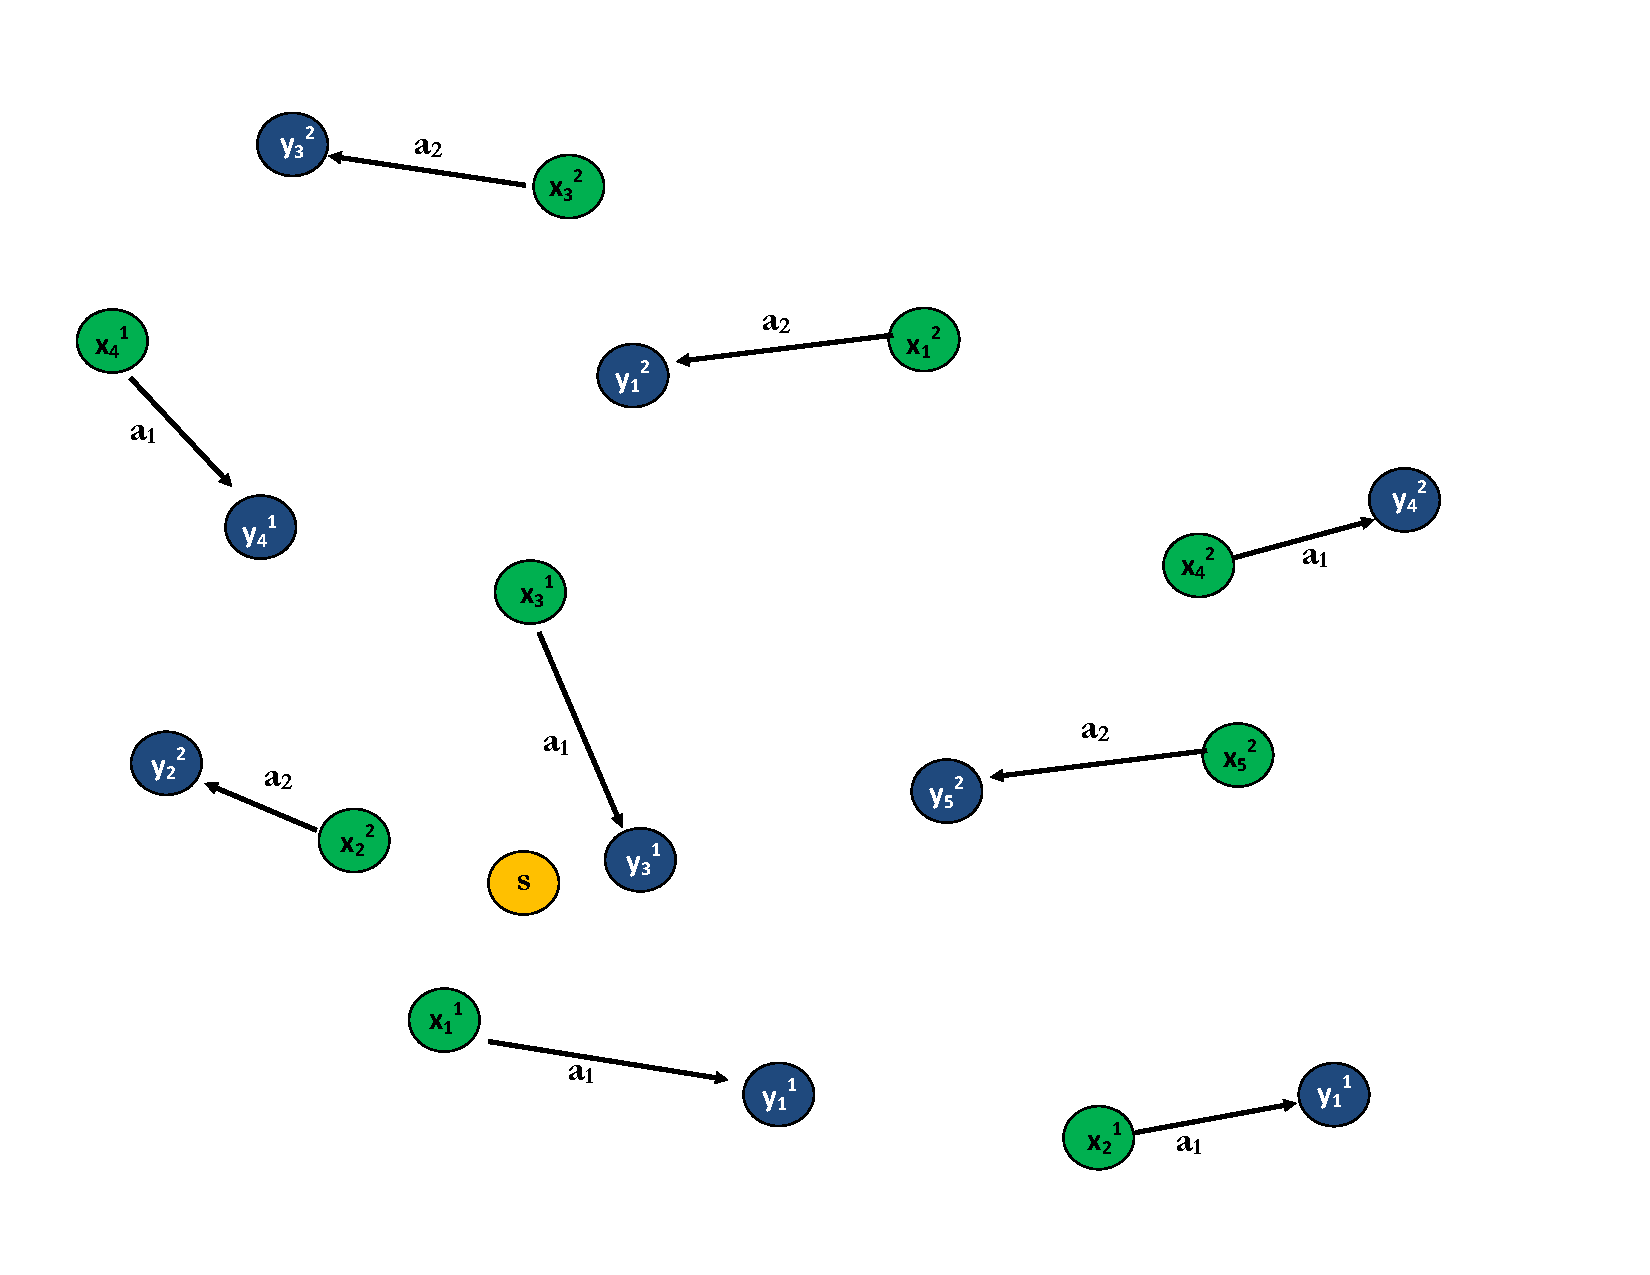
\includegraphics[width=120mm, height=108mm]{figs/kbrlexpl.pdf}
  \caption[Explanation of the the KBRL finite model]{An example set of transitions.
      Arrows are labelled with the action taken.
      For bandwidths near $0$, KBRL assumes $a_1$ takes $s$ to $y^1_1$ and
      that $a_2$ takes $s$ to $y^2_2$ with probability near $1$.}
\end{figure}

$T'$ says that the probability of going from $s$ to an open ball $B$ 
under action $a$ roughly equals the fraction of points in $S^a$ whose 
start is ``similar'' to $s$ and transition into $B$.
The similarity function $\kappa_a(s,s')$ must be nonnegative and decreasing in
$||s - s'||$.
It must also satisfy $\sum_{i < n_a} \kappa_a(s,s^a_i) = 1$.
These properties make $k_a$ usable as a probability function.
These properties also make the Q-Value interpolation a convex combination
of the computed Q-Values.

Ormoneit \& Glynn \cite{kbrl2} discuss a few different forms for the similarity 
function including smoothing kernels, nearest neighbor 
regression, grid-based approximations, and trees.
All of these define similarity in terms of Euclidean distance.
The justification for using such functions is the assumption that the
Q-Values are smooth, that is, that spatial closeness implies value closeness.
But most of the interesting MDPs in RL do not have smooth Q-Values.
For these MDPs, spatial distance is the wrong notion of similarity.
The next chapter discusses this issue in detail and describes the ideal
similarity function.

It is convenient to think of $\kappa(s,s')$ as being the normalized version
of some underlying mother kernel $k(\frac{||s-s'||}{b})$ with bandwidth $b$.
The error in the value function approximation 
has two parts, a bias and a variance term \cite{kbrl}.
The bias is a result of smoothing and the fact that we are estimating
the maximum of a random variable. The bias is increasing in $b$.
The variance is a result of the irregularity of the data and is decreasing
in $b$.

Ormoneit \& Sen \cite{kbrl} also showed that, under some smoothness
assumptions on
the value and reward functions, in the limit of infinite sample transitions
whose starts uniformly cover the reachable state space and a
bandwidth that shrinks at an appropriate rate, the probability of choosing
a suboptimal action from KBRL goes to zero.

\subsection{Approximate KBRL by Stochastic Factorization}
The size of the finite model constructed by KBRL is equal to the number of
sample transitions.
This makes solving it computationally intensive, even when using a sparse
kernel.
Barretto et. al. \cite{kbsf} found that the value iteration can be performed efficiently if
the transition probability matrix is replaced by a low-rank approximation.

The paper computes an approximate stochastic factorization as follows.
Let $T'$ be the $n \times n$ transition matrix KBRL creates for some action,
$a$.
$n - n_a$ columns of $T'$ are entirely $0$ and the remaining
$n_a$ columns contain $\kappa_a(s,s')$ for some pairs of states.
$T'$ is a stochastic matrix (i.e. all its rows sum to one).
Let $\dot{T}'$ be $T'$ with the $0$ columns removed.
$\dot{T'}$ can be approximated as the product of a pair of stochastic matrices $DK$
where $D$ is $n_a \times m$ and $K$ is $m \times n_a$ for some $m < n_a$.
The rank, $m$, of the resulting factorization determines the coarseness of
the approximation.

Barretto et. al. \cite{kbsf} describe a method for constructing $D$ and $K$ using
$m$ representative points $\{\bar s_1, \ldots, \bar s_m\}$ drawn from $S$.
The construction sets $D_{ij} = \kappa(\hat s_i, \bar s_j)$ and
$K_{ij} = \kappa(\bar s_i, s_j)$.
Note that the rows of $D$ and $K$ must be normalized to sum to $1$.
In a follow up paper \cite{ikbsf}, Barretto et. al., show an incremental way
to build the matrices used. They also showed that the approximation
error resulting from stochastic factorization is related to the maximum
distance of a sample point to its nearest representative point.

Stochastic factorization adds a second layer of blurring to the value function
approximation. 
Given the same data, KBSF produces a smoother approximation than the one
produced by KBRL, but if given the same amount of compute time,
KBSF can potentially produce a higher fidelity approximation than KBRL.
For a more thorough discussion of KBSF, see Barretto et. al.'s technical report
\cite{pkbrl}.

\subsection{Discussion of KBRL}
I now conclude this chapter with a high level discussion of the
properties of KBRL and its weaknesses.
The comments below are merely observations and do not correspond to any 
established facts.

I do not know of any theorems about how quickly the policy generated by
KBRL approaches $\pi^*$ as the number of samples grows. 
There are, however, three things that I believe relate to the number of
samples needed to learn an optimal policy.

\begin{description}
\item[Value Function Complexity]
Functions with a high curvature are difficult to represent using a
kernel smoother.
This makes MDPs with bumpy value functions challenging for KBRL.
To get the curvature right, KBRL must be run with a small bandwidth.
To work well with a small bandwidth, KBRL must use a large set
of sample transitions.

\item[Model Dynamic Complexity]
KBRL estimates the transition and reward functions from the sample
transitions.
If these functions are very complicated, estimating them
well will require a large sample set.

\item[Effective State Space Volume]
Let the action-distance between a pair of states $s_1$ and $s_2$ be the
expected number of actions the agent must take to get from $s_1$ to
$s_2$.\footnote{Assuming reachability.}
I consider the effective diameter of the state space to be the maximum
action-distance over all pairs of states.
This quantity is related to the number of sample transitions needed to
cover the space.
KBRL generates solutions that resemble sample transitions stitched together.
This means that for KBRL to generate a particular trajectory, the training
set must contain some transitions near every transition in that trajectory.
It follows that if the time discretization, $\Delta t$, is halved, then the
number of samples needed to get the same level of coverage will increase by
an $O(2^d)$ multiplicative factor, where $d$ is the number of dimensions.
\end{description}

Of the items listed above, only the complexity of the dynamics is
directly related to the ``true'' difficulty of an RL problem.
There is no getting around the need for samples to overcome
uncertainty about the dynamics.

Effective state space volume is not, in and of itself, indicative of the
difficulty of an RL problem.
There is no reason why a control problem should get harder because the
sampling frequency is increased; if anything, it should get easier.
The agent could always just downsample and act as if the sampling
rate did not change.

A possible fix for problems arising from the effective state space volume
is to consider sustained actions.
Instead of creating a dataset of single timestep transitions,
one could create the dataset by holding the action until the state has
moved by some amount, $\epsilon$.\footnote{There should also be a
timeout for how long the action is sustained in case the action has no effect.}
The justification for doing this is the belief that the optimal policy will
not require the agent to rapidly switch between actions.
I suspect that that the optimal $\epsilon$ is related to the density of
samples being collected.

The purpose of this thesis is not to tackle the problem of effective
state space volume, so
a formal argument about when sustained actions are appropriate is left for
future work.
This thesis does, however, use sustained actions  in the experiments
presented in the results section.

This thesis is concerned with alleviating the problems that come from
value function complexity.
Value function complexity, as defined above, is not just a product of
MDP difficulty; it can also come from the choice of representation.
The next chapter shows the role representation plays in value function
complexity and describes the characteristics of a good representation.
%% This is an example first chapter.  You should put chapter/appendix that you
%% write into a separate file, and add a line \include{yourfilename} to
%% main.tex, where `yourfilename.tex' is the name of the chapter/appendix file.
%% You can process specific files by typing their names in at the 
%% \files=
%% prompt when you run the file main.tex through LaTeX.
\chapter{Changing Representations}
The previous chapter described KBRL, a value-iteration
algorithm for solving continuous RL problems.
KBRL uses local averaging to create an approximate value function.
This chapter demonstrates by example how, on some simple MDPs,
local averaging creates
problems---problems that can be fixed by a change in representation.
It then gives a more formal description of the types of MDPs that
cause difficulties.
The chapter concludes with a brief overview of related work from the
representation discovery literature.

\section{Motivating Example}
The discussion section of the background chapter claimed that MDPs with
bumpy value functions are difficult to solve using KBRL.
This section presents a concrete example to show why this is so, and how 
it can be fixed by a change in representation.

Consider the MDP \textit{TWO-ROOM} pictured in Figure 3-1.
\textit{TWO-ROOM} describes an agent in a world with two rooms partially
separated by a thin wall.
The agent is free to move through the open space of the world but cannot
pass through the wall.
A region in one room is marked as the goal.
The agent receives a reward of $-1$ for every time step that it is not in
the goal and a reward of $0$ when it is in the goal.\footnote{Think
of the goal as an absorbing terminal state. Once the agent gets there,
it stays there.}

\begin{figure}[!!!ht]
  \centering
    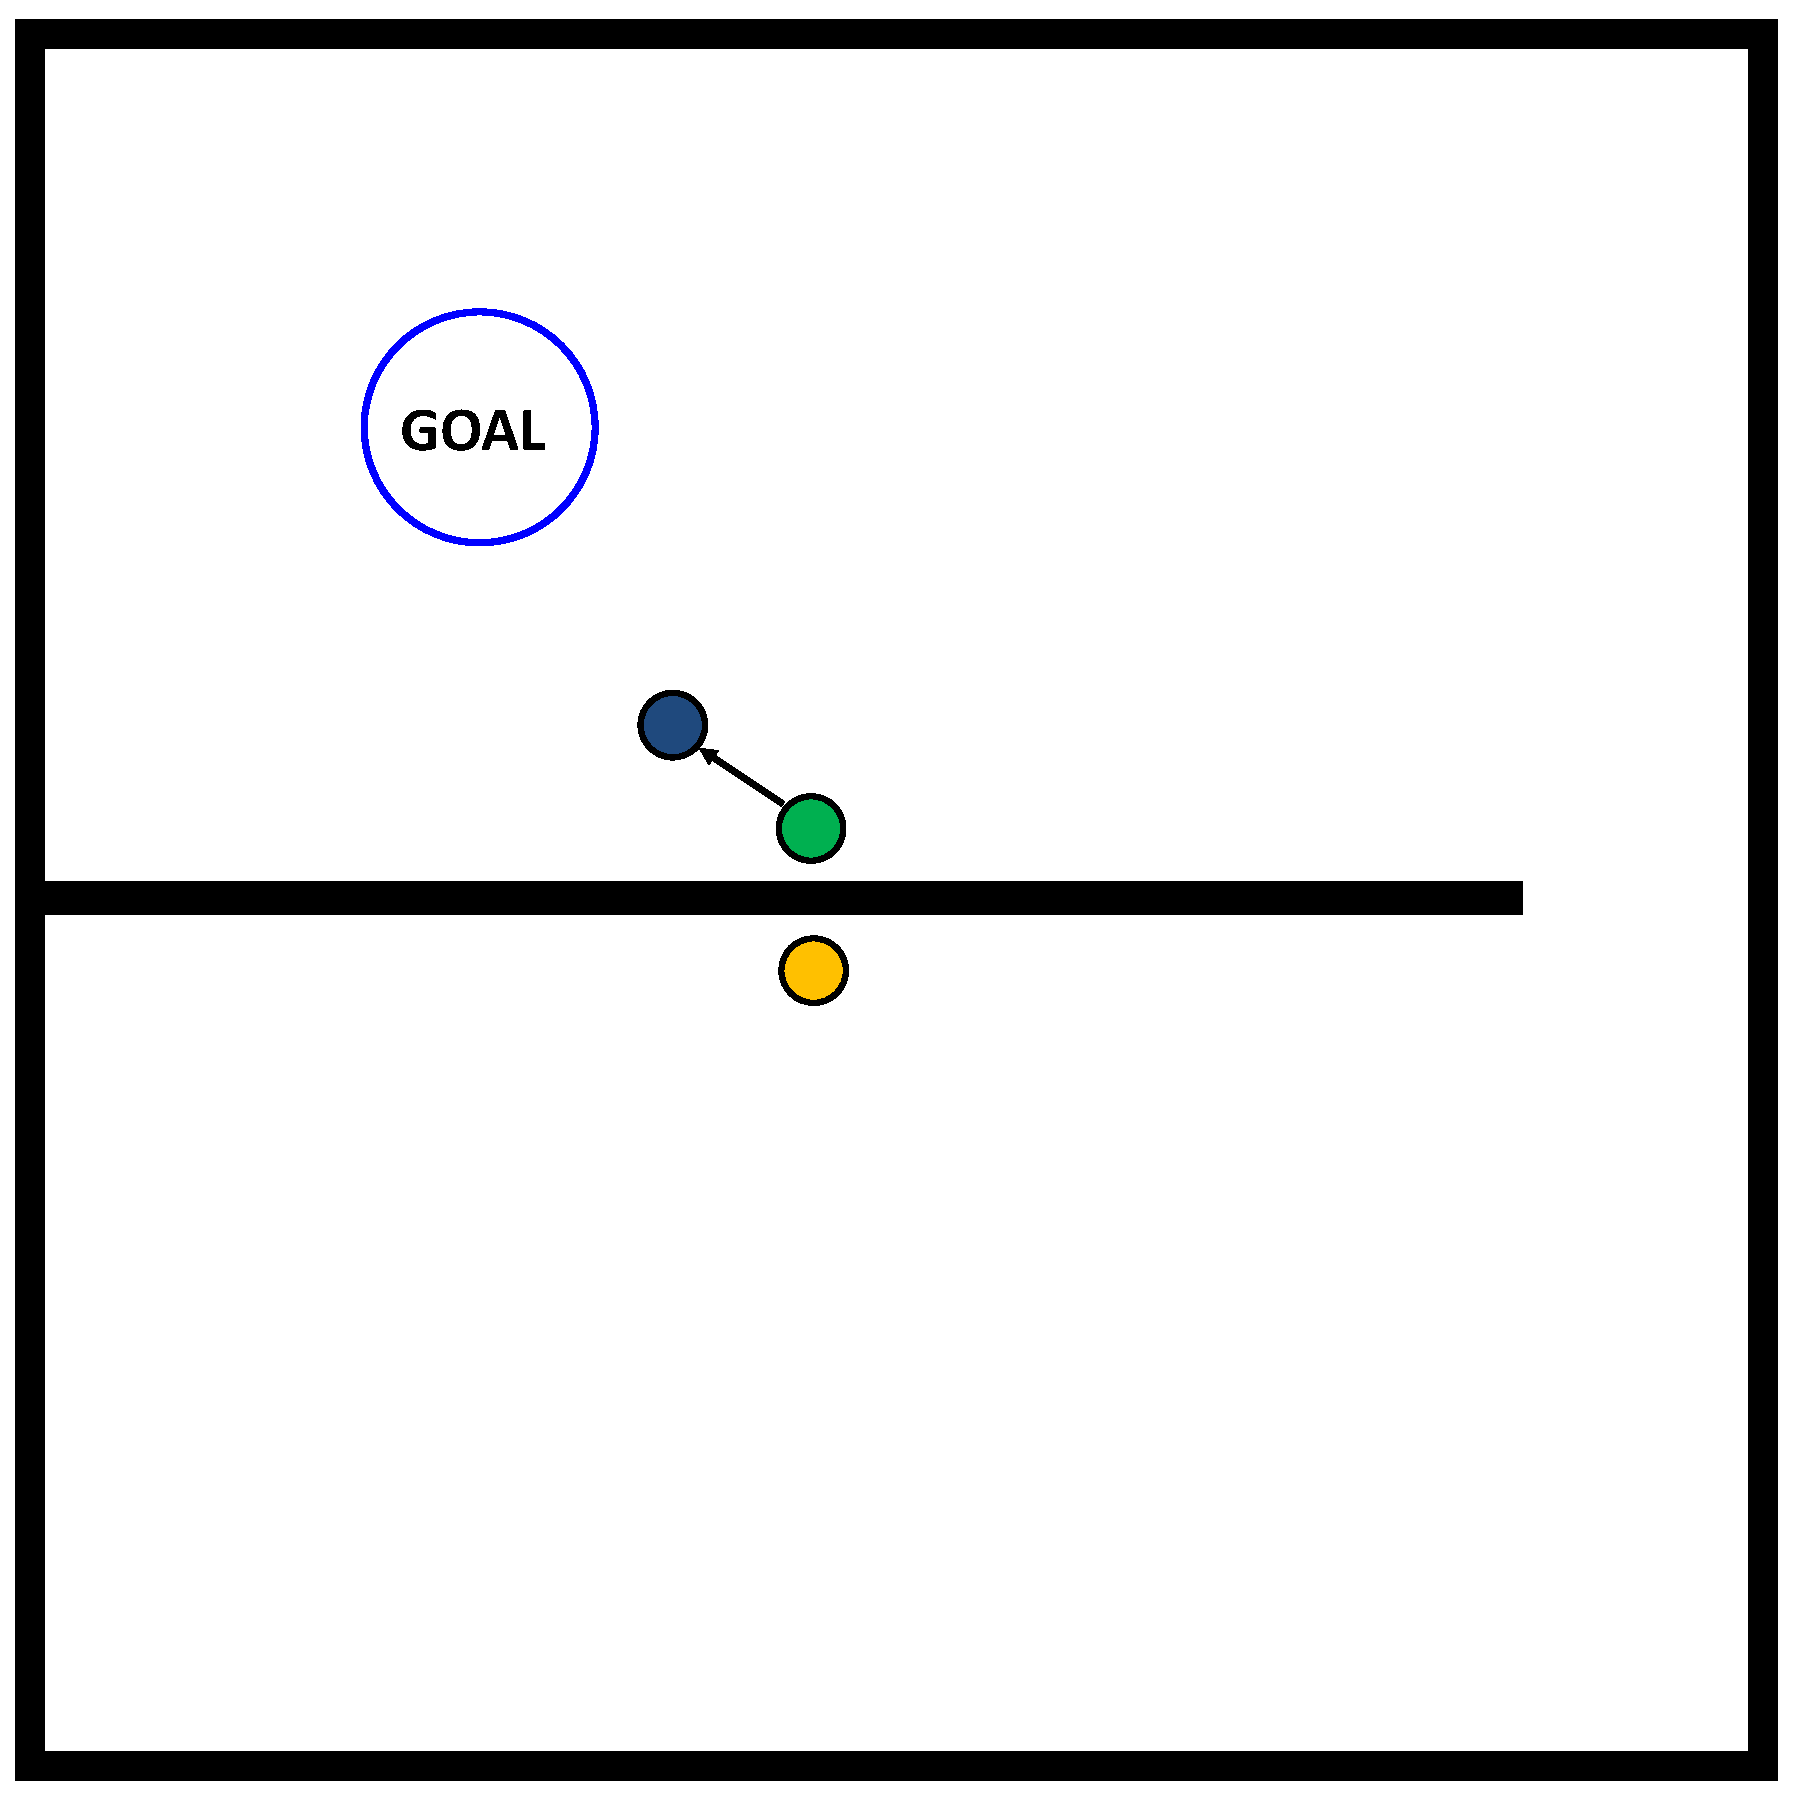
\includegraphics[width=50mm]{figs/tworoom.pdf}
  \caption[The state space of \textit{TWO-ROOM}]
  {The state space of \textit{TWO-ROOM}.
    In this MDP, it would be undesirable to allow a sample transition
    in the top room affect the model of the bottom room.}
\end{figure}

In \textit{TWO-ROOM}, the optimal policy has the agent navigate 
directly to the goal.
Thus, the value of a state is decreasing in the length of the shortest
path from it to the goal.
This means states that are spatially close together, but on opposite sides
of the wall, have significantly different values (see Figure 3-3).
Faithfully representing the steep drop in value across the wall is
necessary for solving \textit{TWO-ROOM}.
To keep KBRL from smoothing out the value cliff, one would need to use
a small bandwidth.
Compensating for the variance that comes from working with
small bandwidths requires using a large set of sample transitions.
This makes the domain much harder for KBRL than it ought to be.

\begin{figure}[!!!ht]
  \centering
    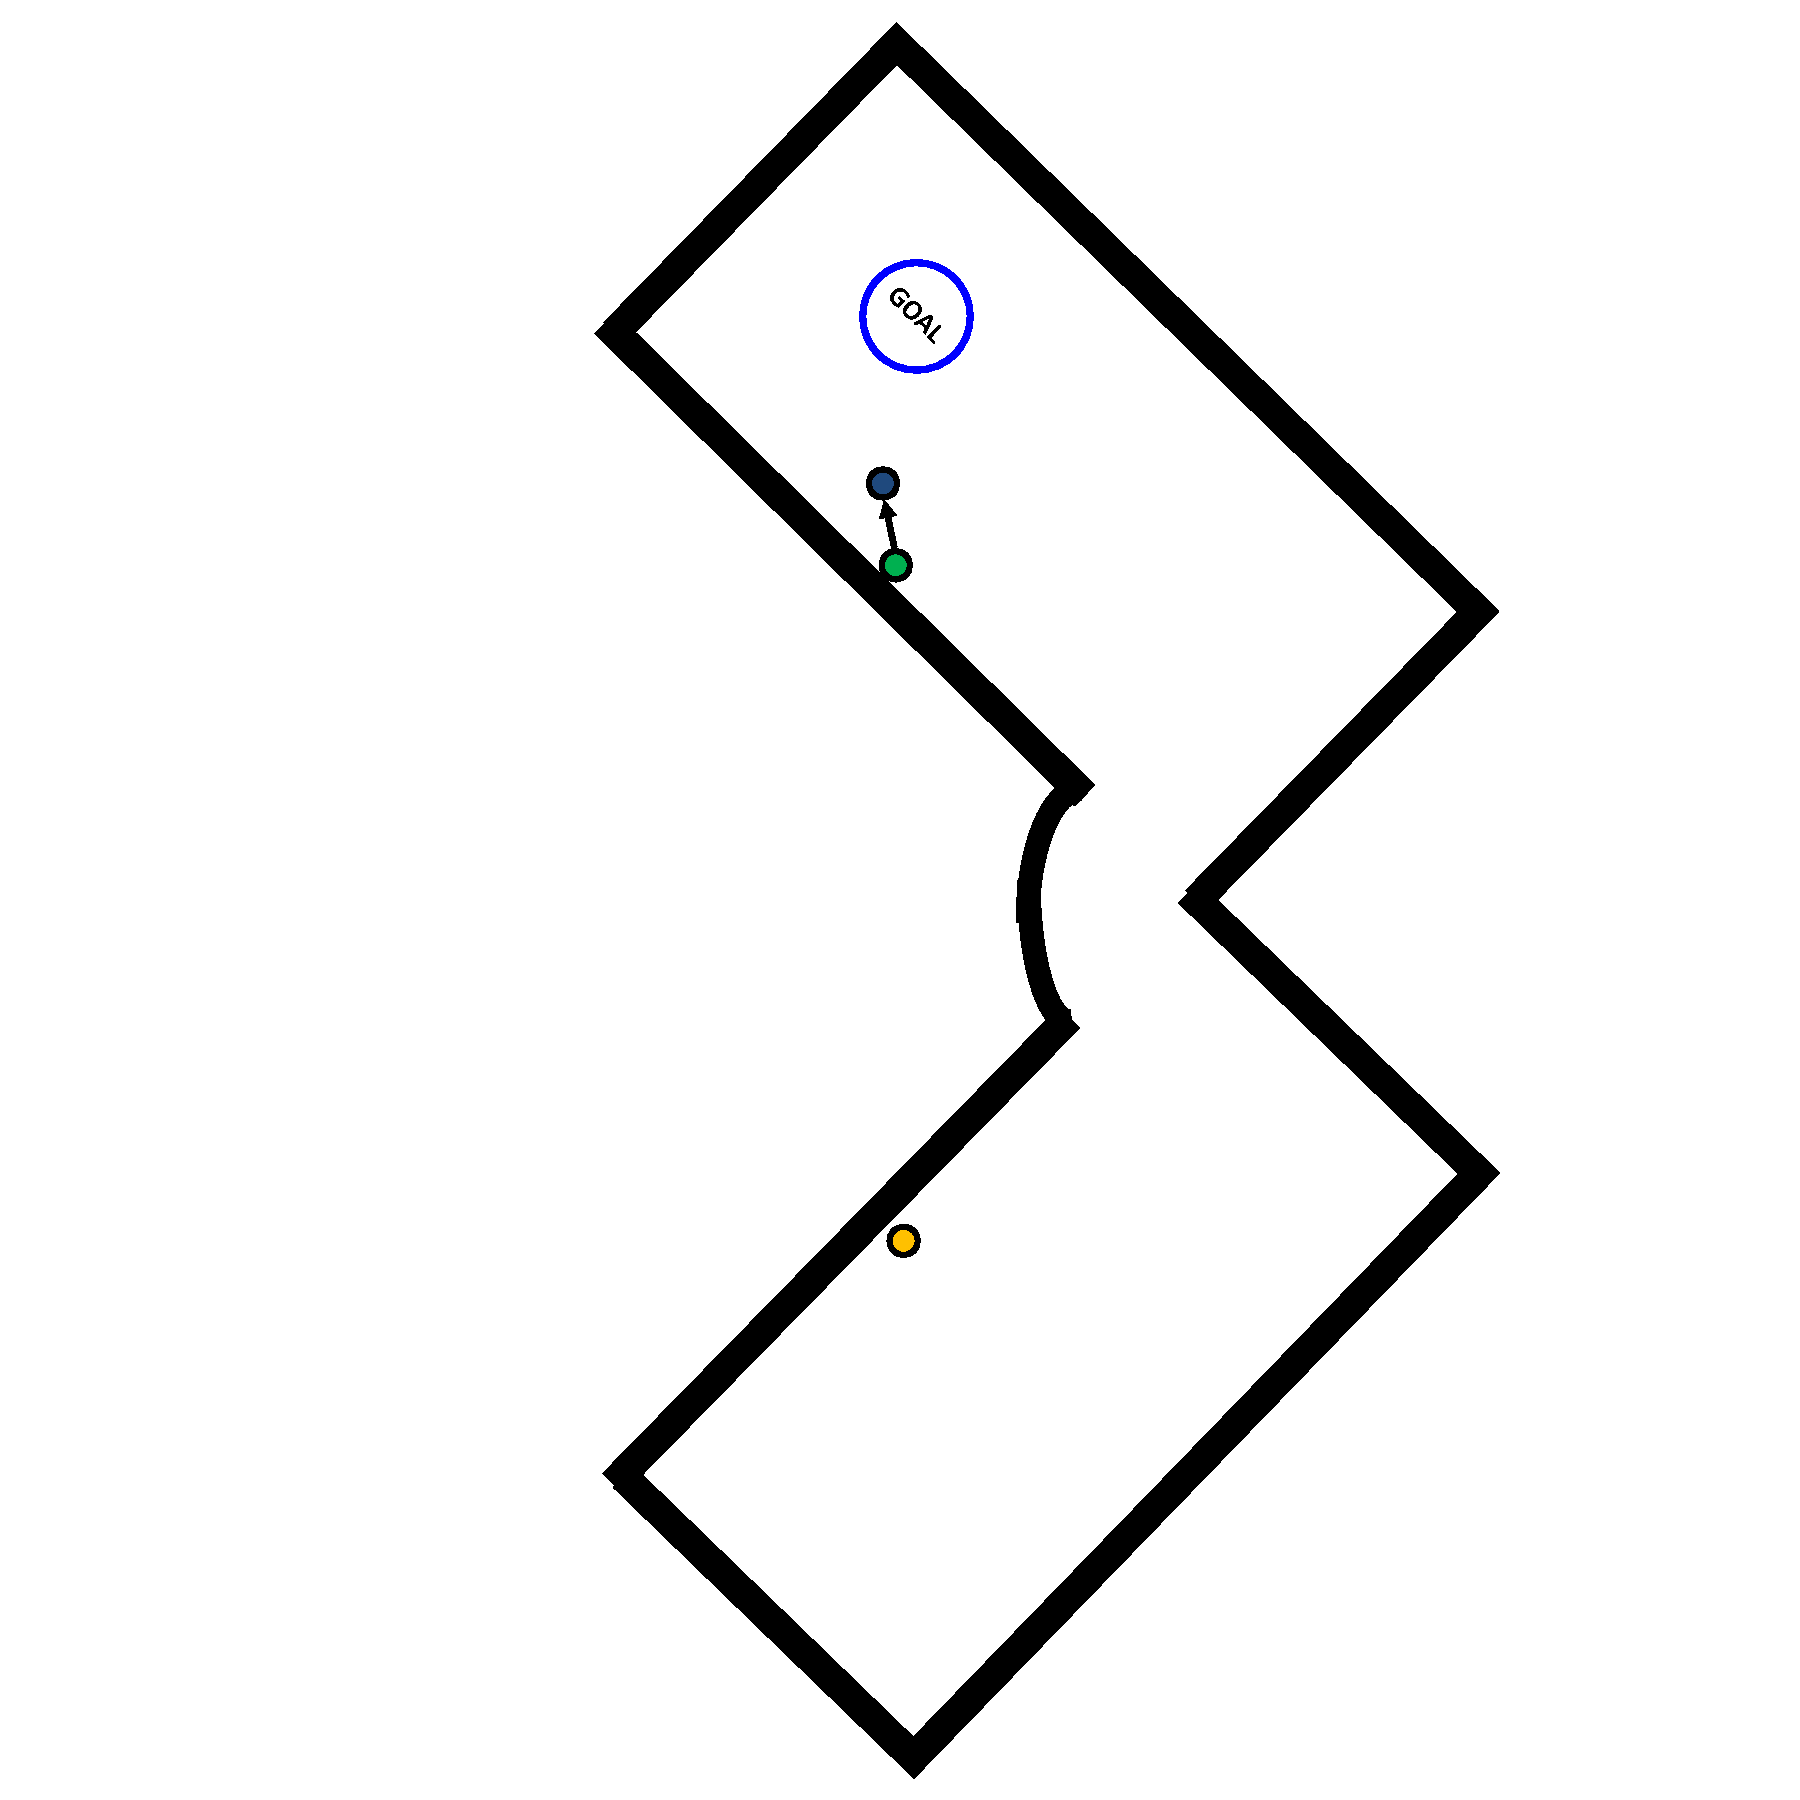
\includegraphics[width=90mm]{figs/tf2room.pdf}
  \caption[Alternative representation for the state space of
      \textit{TWO-ROOM}]
      {An alternative representation for the state space of
\textit{TWO-ROOM}. In this representation there is little risk of
averaging across the wall.}
  \label{fig:tf2rm}
\end{figure}

Now consider a representation for the state space where the wall is
``opened up'' so that states on opposite sides of it are no longer close
(Figure 3-2).
In this representation, the distance between two points says something
about their similarity.
This makes local averaging safe to do with a much larger bandwidth and
far fewer points.

\begin{figure}[!!!ht]
  \centering
    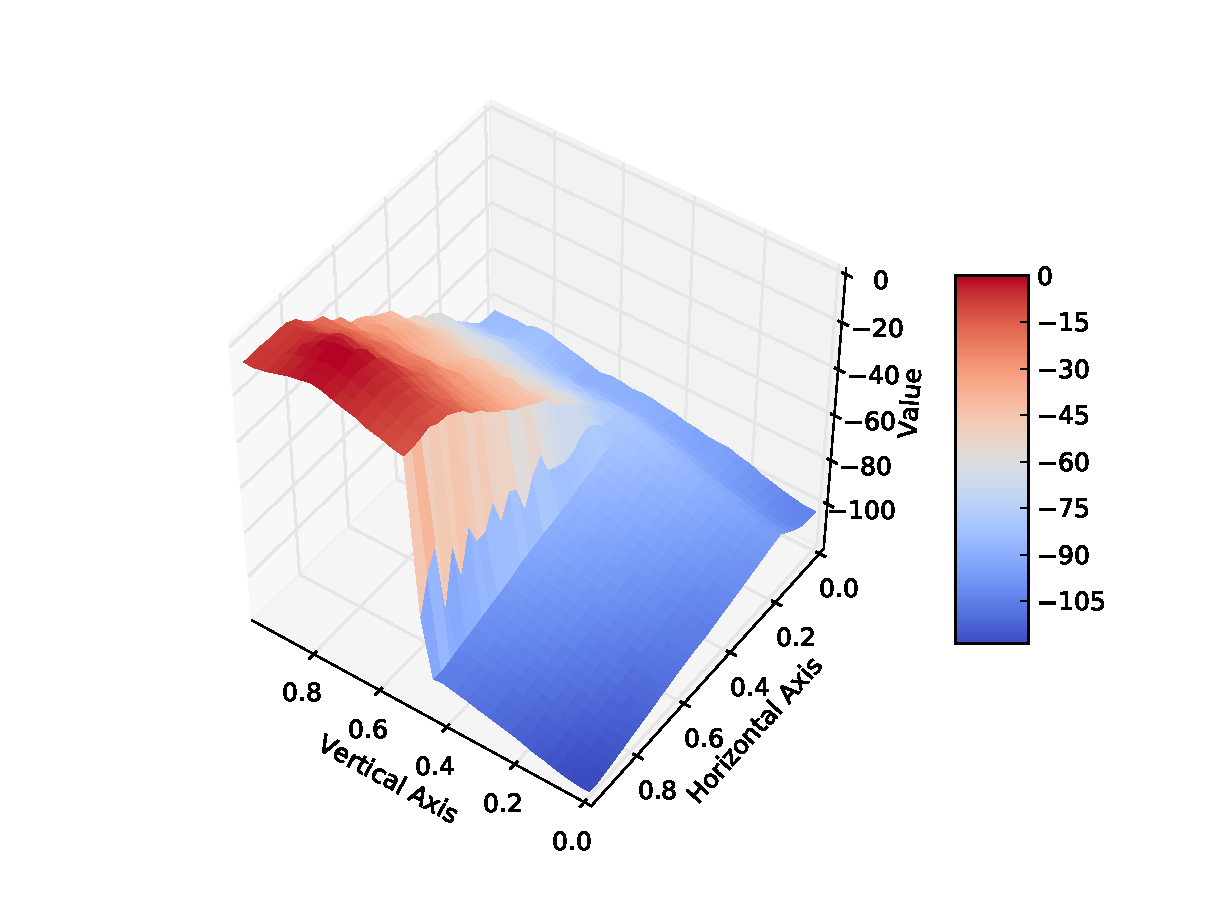
\includegraphics[width=110mm]{figs/true2rmvf.pdf}
  \caption[\textit{TWO-ROOM} value function learned using small bandwidth]
  {The value function of \textit{TWO-ROOM} as approximated by
  KBRL in the original space with a bandwidth of $.01$. It captures the
  discontinuity adequately. Notice the ripples in the top room. These are
  artifacts of the small bandwidth.}
  \label{fig:og2rm}
\end{figure}

\begin{figure}[!!!ht]
  \centering
    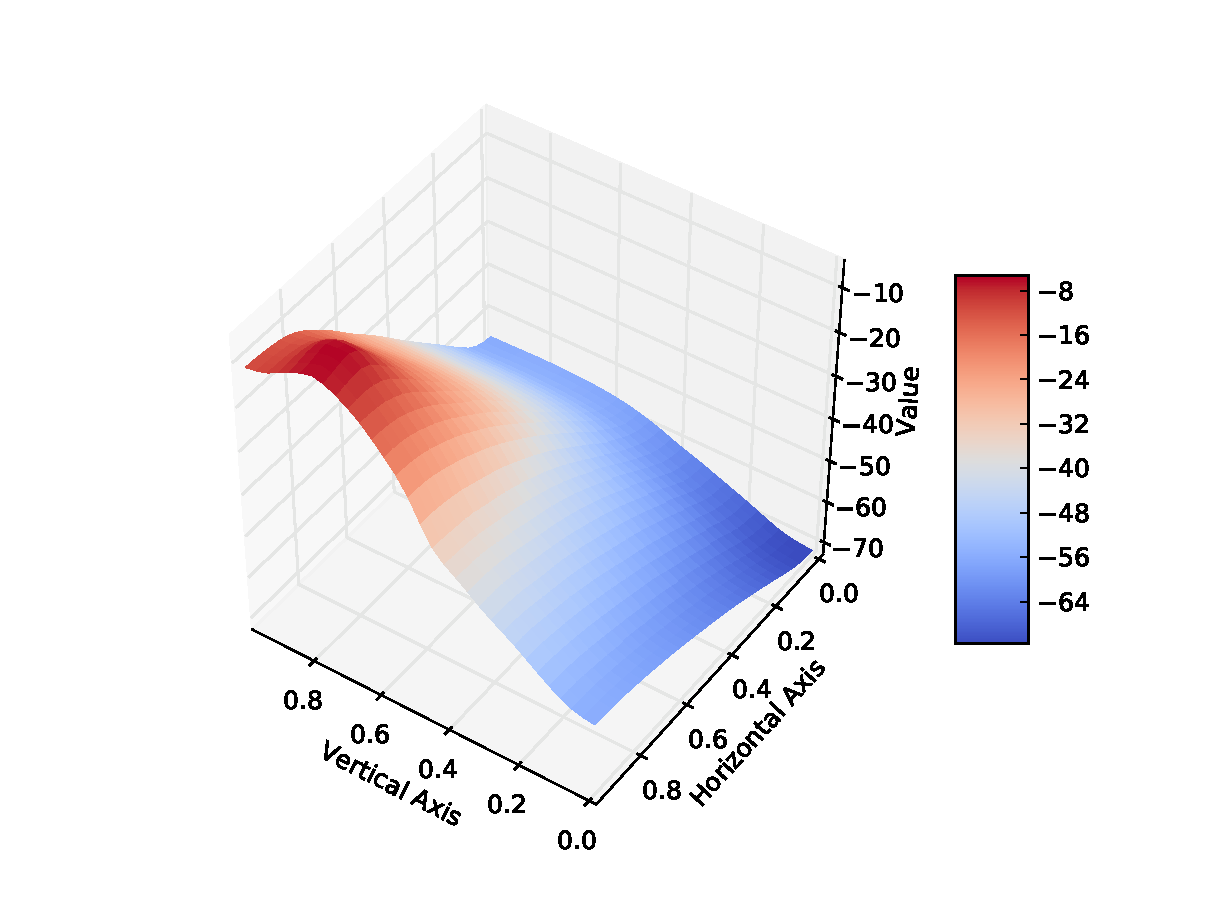
\includegraphics[width=110mm]{figs/blur2rmvf.pdf}
  \caption[\textit{TWO-ROOM} value function learned using large bandwidth]
  {The value function of \textit{TWO-ROOM} as approximated by
  KBRL in the original space, this time with a bandwidth of $.06$.
  Note how poorly it models the wall.
  The policy that results from this value function
  has the agent attempt to walk through the wall.}
  \label{fig:bl2rm}
\end{figure}

\begin{figure}[!!!ht]
  \centering
    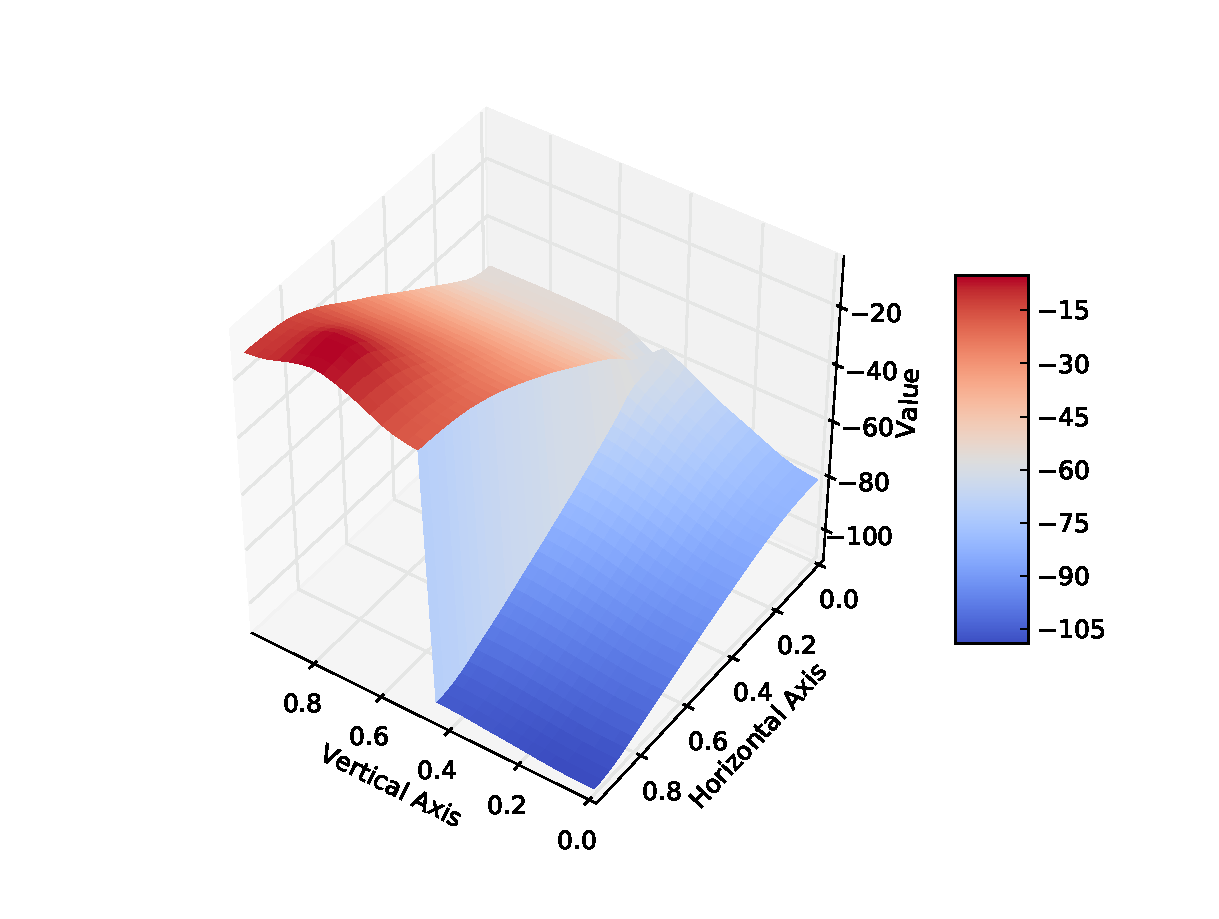
\includegraphics[width=110mm]{figs/tf2rmvf.pdf}
  \caption[\textit{TWO-ROOM} value function learned in the transformed space]
  {The value function of \textit{TWO-ROOM} approximated by
  KBRL in the transformed space and mapped back to the original toplology
  (bandwidth of $.06$).
  This captures the discontinuity well and has no ripples.
  All three plots (3-3, 3-4, 3-5) above were created using the same
set of sample transitions.}
  \label{fig:tfv2rm}
\end{figure}

\section{Discussion}
By any reasonable measure, \textit{TWO-ROOM} is a simple domain,
yet it poses a challenge for KBRL simply because its value function
has a discontinuity.
KBRL is intended for problems with smooth value functions, so
it is understandable that it would do poorly in this domain.
The failure is not one of technique, but of representation.
The original representation of the MDP is not well suited for
representing the value function.
After a simple transformation, the domain becomes easy for KBRL.

The discontinuity in \textit{TWO-ROOM}'s value function comes from
the local connectivity of the state space;
this is not the only way discontinuities arise.
Discontinuities can also come from non-local properties of the MDP.
Consider the following minor modification to \textit{TWO-ROOM}:
the agent can run through the wall if it hits it with enough momentum,
but building up the necessary momentum requires the agent to accelerate
through some distance, $\delta$.
In this formulation, states where the agent is on pace to break though the wall
have a very different value from the ones where it isn't.
Note that these states may be arbitrarily close to each other and up to
a distance of $\delta$ from the wall.\footnote{To see another discontinuity
of this form, see MountainCar in the Results chapter.}
There is no local information that can help differentiate these states.

Transition dynamics are not the only possible cause of roughness in
the value function.
Value cliffs can also result from the underlying reward structure of the MDP.
An example of this is \textit{TWO-ROOM} where the wall is not a physical
barrier but a region of low reward.
With this modification, there is nothing about the topology of the space that
would suggest a discontinuity but the value function is as if there is a wall.

Many of the benchmark problems in the reinforcement learning literature are
like \textit{TWO-ROOM};
their value functions are smooth but for a handful of discontinuities.
This suggests that they too could benefit from a change in representation.
In \textit{TWO-ROOM} we were able to use domain knowledge to engineer a new
representation. This is not always possible or desirable.
Ideally, the agent would discover a good representation in the process
of solving the problem.

\section{The Best Representation}
The previous sections provide a high level discussion of the advantage of
changing representations.
The existence of regions of the state space where the value function
changes rapidly is problematic for KBRL.
Our solution is to transform the state space in a way that smooths out the
value function.
We now make these ideas concrete and attempt to gain insight about the
best possible transform.

Let $f:X \to Y$ be a non-constant, Lipschitz-continuous\footnote{
Lipschitz-continuity roughly corresponds to having a bounded slope.
A function, $f$ is Lipschitz-continuous if there exists a $K$ such that
for all $x$, $x'$ in the domain of $f$,
$K \geq \frac{|f(x) - f(x')|}{\|x - x'\|}$.
A $K$ satisfying this equation is called a Lipschitz constant for $f$.},
and bounded function with compact, connected support.
Denote the diameter of the support as $diam(X) = \max_{x,x' \in X}||x - x'||$
and let $f_{max}$ and $f_{min}$ denote the maximum and minimum values 
respectively of $f$ on $X$.
Let $K_f$ denote the smallest Lipschitz constant for $f$.

\begin{definition}
The \textbf{wrinkliness} of $f$ is
$w(f) = K_f \cdot \frac{diam(X)}{f_{max} - f_{min}}$.
\end{definition}

Consider the function $g(x) = \mathrm{log}(x^2-7x+20)$ with domain $[1,100]$.
The extrema of $g$ are $g_{min} \approx 2.05$ and that $g_{max} \approx 9.14$.
The maximum slope of $g$ is $\approx .36$.
From this we can calculate that $w(g)\approx.36*(100-1)/(9.14-2.05) = 5.01$.

The wrinkliness of a function is the ratio of its maximum slope to the
minimum slope it would need to pass through the extrema on its domain.
Wrinkliness is a measure of how non-linear a function is.
Note that $w(f) \geq 1$. Call $f$ \textbf{wrinkle-free} if $w(f) = 1$. 
The only way $f$ can be wrinkle free is if it attains its global extrema
at points separated by the diameter and its slope never exceeds
$\frac{f_{max} - f_{min}}{diam(X)}$.

\begin{definition}
The \textbf{inverse target slope} of $f$ is
$\mu_f = \frac{diam(X)}{f_{max} - f_{min}}$.
\end{definition}

An example of a wrinkle-free function is $f(x) = c x + d$ for some
constants $c$ and $d$. All wrinkle-free functions in one-dimension are of
this form. In higher dimensions, wrinkle-free functions can be more
complicated.

Now consider a transform $\Phi: X \to X'$ ($X'$ compact and connected)
satisfying $f(x_1) \neq f(x_2) \implies \Phi(x_1) \neq \Phi(x_2)$.
Let $f_\Phi : X' \to Y$ be the function satisfying $f_\Phi(\Phi(x)) = f(x)$.
The existence of $f_\Phi$ follows from the constraint that $\Phi$ not map
points with the different values to the same point.
If $f_\Phi$ is Lipschitz-continuous, we can define wrinkle-ironing transforms
as follows:

\begin{definition}
$\Phi$ is a \textbf{wrinkle-ironing transform (WIT)} if $w(f_\Phi) \leq w(f)$.
\end{definition}

Consider the transform $\Phi_{\log}(x) = \log(x)$.
Applying $\Phi_{\log}$ to the domain of $g$ above gives the new domain
$[0,\log(100)]$.
The $g_\Phi$ satisfying $g_\Phi(\Phi_{\log}(x)) = g(x)$ is
$G(x) = \log(e^{2x}-7e^x+20)$. It has the same extrema as $g$ and a
maximum slope of $2.61$.
From this we can calculate that
$w(G)\approx2.61*\mathrm{log}(100)/(9.14-2.05)=1.69$.
This means $\Phi_{log}$ is a wrinkle ironing transform for $g$.

\begin{figure}[!htb]
  \minipage{0.5\textwidth}
    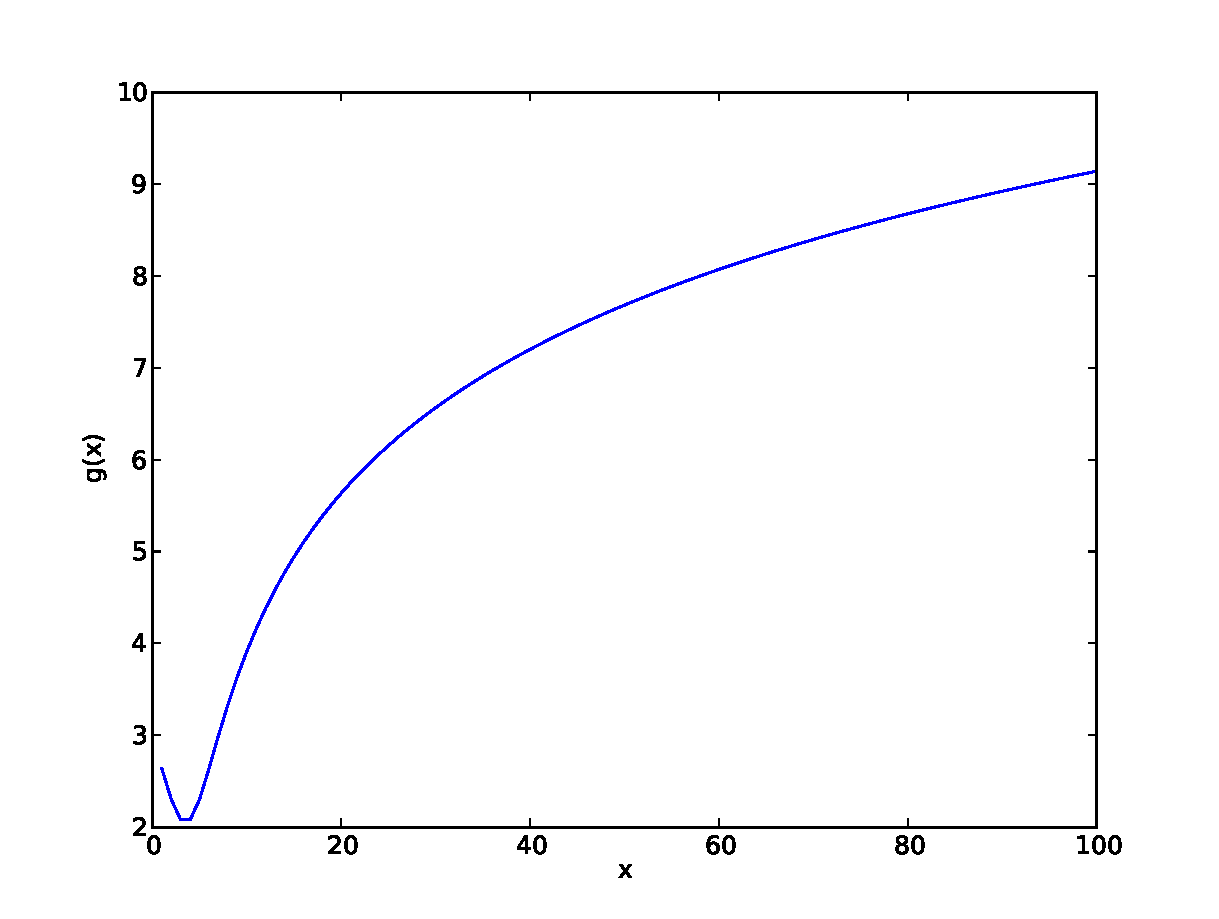
\includegraphics[width=\linewidth]{figs/gp1.pdf}
  \endminipage\hfill
  \minipage{0.5\textwidth}
    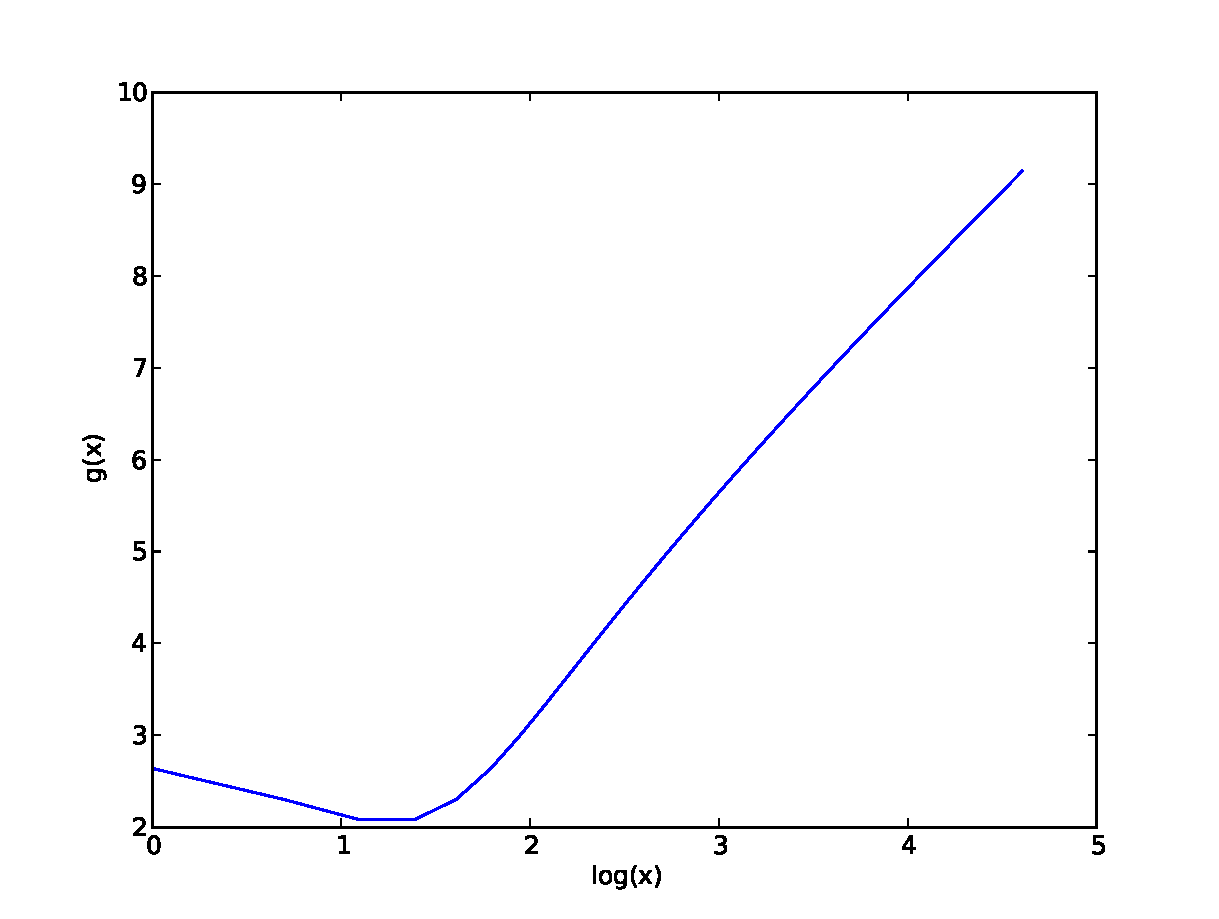
\includegraphics[width=\linewidth]{figs/gp2.pdf}
  \endminipage
\caption[Wrinkle-Ironing Transform Example]{On the left, $g(x)$ plotted on its
  original domain. On the right, $g(x)$ plotted against $\log(x)$.
  Note how the WIT straightened out the function.}
\end{figure}

Local-averaging kernel-smoothers work by assuming the function being
approximated is locally flat.
As a result, the only function they can represent without error is
the constant function, $f(x) = c$ for some $c$.
In the special case where the domain is unbounded and the sample points uniformly
cover the domain, kernel-smoothers can also represent lines without error.
\footnote{When the domain is bounded the kernel-smoother produces an
approximation that is biased at the boundaries.
The implications of this are discussed in detail in the next chapter.}
This means one can use wrinkliness as a measure of how poorly a
kernel smoother will represent a function.

KBRL approximates the Q-Values of an MDP using kernel smoothers of the form
$k(\frac{||s - x||}{b})$.
If we assume that wrinkliness is a reasonable measure of fit quality,
it follows that without lowering the bandwidth, one can get a higher
fidelity approximation by applying a wrinkle-ironing transform,
$\Phi$, to the state space and working with
$k(\frac{||\Phi(s) - \Phi(x)||}{b})$.
Since it may be the case that no single transform can iron the wrinkles
in all the Q-Values, one should use a separate transform $\Phi^a$ for
each action, $a$.

Note that applying a transform that stretches the state space uniformly in
all directions is equivalent to shrinking the bandwidth.
We exclude will such transforms by adding the constraint that the
transforms not increase the diameter of the state space.

All this leads us to the conclusion that the best possible transform
is the wrinkle-free $\Phi^{a^*}(s) = \mu_{Q^a} \cdot Q(s,a)$, we define
this to be \textbf{the Platonic Transform}.
This is a disheartening result;
it suggests one needs to know the Q-Values to produce a transform that makes
it easy to approximate the Q-Values.
The next chapter introduces an algorithm that attempts to bootstrap a
solution to this problem, iteratively approximating the Q-Values then the
transform.

A possible concern is that transforming the state space in this way may alter
the optimal policy.
The transform $\Phi^*$ described above is a $Q^*$-irrelevance abstraction
\cite{lietal} since
$\Phi^*(s_1) = \Phi^*(s_2) \implies Q(s_1, a) = Q(s_2, a)$ for all $a$.
Q-learning with a $Q^*$-irrelevance
abstraction converges to the optimal state-action value function in the
underlying MDP. 
This means using $\Phi^*$ in KBRL will not lower the solution quality.

\section{Related Work}
Representation discovery is not a novel concept.
The past decade has seen several representation discovery algorithms
in a number of different settings.
The following are the ones most closely related to this thesis,
presented in chronological order.

\begin{description}
\item[ST-Isomap]
\cite{jenkins} is an extension of Isomap \cite{tenen} that takes temporal
information into account.
It uses a modified nearest neighbours algorithm to construct a graph from
the dataset.
It then unfolds the graph using MDS \cite{mds} on the matrix of shortest-path
distances.

\item[Action-Respecting Embedding] \cite{bowling} constructs a graph from
the set of sample transitions using nearest neighbours with the
neighbourhood sizes determined by the effect of an action.
It then unrolls and morphs the graph using a semidefinite program whose
constraints ensure that neighbourhoods are preserved and that each action
corresponds to a rotation-plus-translation.

\item[BEBF] \cite{parr} is an algorithm for discovering a set of basis
functions for use in a linear approximation architecture. It iteratively
adds new bases using the approximation error from the old bases.

\item[PVFs] \cite{pvf} constructs a graph embedding using nearest
neighbours on the dataset then attempts to represent the value function
in terms of the eigenfunctions of the graph Laplacian.
PVFs can be computationally intensive to create, but recent work on
Incremental SFAs \cite{incsfa} has made it more tractable.

\item[Predictive Projections] \cite{sprague} finds a linear transformation
that projects the original space into a space where state values are more
highly correlated.
\end{description}

These algorithms all had considerable success in dealing with the problems
they were designed to address, but they are not versatile enough to
generalize to other types of problems. For instance, they all fail on some
version of \textit{TWO-ROOM} presented above.

The algorithms that build a graph representation (ST-Isomap, PVFs, and ARE)
can only create representations that fix discontinuities that come from the
local topology of the state space.
They cannot deal with the case where the agent can run through the wall or
where the wall is replaced by a region of low reward.
It is not possible to build a representation that is universally useful
without considering the reward function.
ST-Isomap and PVFs are further limited by the fact that the abstractions they
produce are neighbourhood preserving---they do not stretch or squash the
domain.
One can imagine cases where the best transform involves distorting the state
space.
Consider, for instance, \textit{TWO-ROOM} modified so that the vertical axis
is measured in meters and the horizontal axis is measured in miles.
A good transform would stretch the axes so that the units matched.

Predictive Projection is severely limited by the fact that it only finds linear
transformations. Few problems of interest can be represented well after a
linear transformation. Predictive Projection cannot make a better
representation for any version of \textit{TWO-ROOM}.

BEBF does not learn a representation of the state space, instead it
learns a basis for representing the value function.
BEBF is similar in spirit to what we are trying to accomplish:
it involves iteratively approximating the value function then updating the
representation; however, since BEBF is parametric, the bases
it considers are tied to the native representation of the problem.

None of the algorithms above have been applied in a non-parametric
reinforcement learning setting. 
This makes it difficult to compare them to the work presented in this thesis.
To the best of my knowledge, there is no literature on non-parametric
representation learning.
Thus, results in this thesis are only compared against the results of
KBRL and KBSF.

Now that the problem of representation discovery has been sufficiently
motivated, we can proceed to describing an algorithm for it.

%% This is an example first chapter.  You should put chapter/appendix that you
%% write into a separate file, and add a line \include{yourfilename} to
%% main.tex, where `yourfilename.tex' is the name of the chapter/appendix file.
%% You can process specific files by typing their names in at the 
%% \files=
%% prompt when you run the file main.tex through LaTeX.
\chapter{Transforming For Improved Fit}
The previous chapter showed that the quality of the solution generated by KBRL
can be improved by transforming the state space of the MDP.
The chapter also showed that constructing a transform that makes the value
function easier to represent requires one to already know the value function.

We now describe an algorithm that attempts to solve this chicken-and-egg
problem iteratively. Section 1 proposes a novel curve-fitting framework,
Fit-Improving Iterative Representation Adjustment (FIIRA),
which takes a regression scheme and a transform generator, and produces a
more powerful regression scheme.
Section 2 describes a specific transform generator for use in FIIRA.
Section 3 discusses the results of combining that transformer with a kernel
smoother.
Section 4 describes an FIIRA approach to KBRL.
Finally, Section 5 provides some implementation considerations.

\section{Fit-Improving Iterative Representation Adjustment}
The problem statement of curve-fitting is as follows: given a set of training
points, $D = \{(x_i,y_i)\ |\ i = 1, \ldots, n\}$, of point-value pairs with
$y_i = f(x_i)$ for some function $f : X \to \mathbb{R}$,
produce a function $\tilde f$ to approximate $f$ well, for some measure of
approximation quality.

A regressor, $r$, is a procedure for producing fits from some space of
functions, $\mathcal{F}_r$.
If $f$ is not well approximated by any function in $\mathcal{F}_r$,
this fit is guaranteed to be poor.
One way to fix to this problem is to transform the domain of $f$ and work in a
space where $f$ \textit{is} well approximated. Choosing such a transform
requires prior knowledge or assumptions about $f$.

What can one do if no information about $f$ is available?
Ideally, one would infer a transform directly from the data.
An interesting way to go about doing this would be to pass $D$ to the
regressor,
then use the approximation produced to guess a transform $\Phi$ such that
$f_\Phi$ is in or near $\mathcal{F}_r$.
Algorithm 1 describes a framework for doing this.
The procedure takes as input a dataset, $D$; a regressor, $REGR$;
and a transform generator, $TF$.

\begin{algorithm}
\caption{Iterative Representation Adjustment for Improved Fit}\label{FIIRA}
\begin{algorithmic}[1]
\Procedure{FIIRA}{$D,\ REGR,\ TF$}
	\State $\Phi_0 \gets x \mapsto x$
          \Comment{The identity transform}
	\State $i \gets 0$
        \State $D_0 \gets D$
	\Repeat
		\State $\tilde f_{i+1} \gets REGR(D_i)$
		\State $\Phi_{i+1}\gets TF(\tilde f_{i+1}, D_i)$
		\State $i \gets i+1$
                \State $D_i \gets \{(\Phi_{i+1}(x), y)\ |\ (x,y) \in D_{i-1}\}$
	\Until{$\tilde f_{i+1} \approx \tilde f_i}$
           \Comment{Or until some measure of error minimized}
	\State \textbf{return} $x \mapsto f_{i+1}(\Phi_{i+1}(x))$
\EndProcedure
\end{algorithmic}
\end{algorithm}

It may not be immediately clear what leverage this technique has to offer.
To see what it can do, consider the case where the regressor
creates polynomial fits of order $p$ and the transform generator
creates polynomial transforms of order $q$.
Applying $k$ iterations of FIIRA will yield a polynomial fit of order
$p + kq$.

I was unable to find anything like FIIRA in the function approximation
literature so I cannot cite any relevant theorems or results.
A formal analysis of the properties of FIIRA
is outside the scope of this thesis and is left for future work.
What follows is an empirical study of FIIRA for the special
case where the regressor is a local-averaging kernel smoother
and the transform generator is the Wrinkle-Ironing Transformer
described below.

\section{Dimension-Adding WIT}
The regressor used in KBRL is a local-averaging kernel smoother.
An FIIRA approach to KBRL requires a transformer that makes functions
easier to represent by kernel smoothing.
If we accept wrinkliness as a measure of representation difficulty,
it follows that the desired transformer is one that produces
Wrinkle-Ironing Transforms.
WITs stretch out the parts of the space where a function is steep
and squash the parts where it is flat.
I now describe a WIT that does this by adding a dimension to the domain.

Consider a transformer which, given a function $f$ with domain $X$, 
maps every $x \in X$ to $x | f(x)$ (the bar represents concatenation).
The transform generated stretches $X$ into $d+1$ dimensions in a way that
pulls apart points that differ in value.
Figure 4-1 demonstrates how this works.

\begin{figure}[!htb]
  \minipage{0.5\textwidth}
    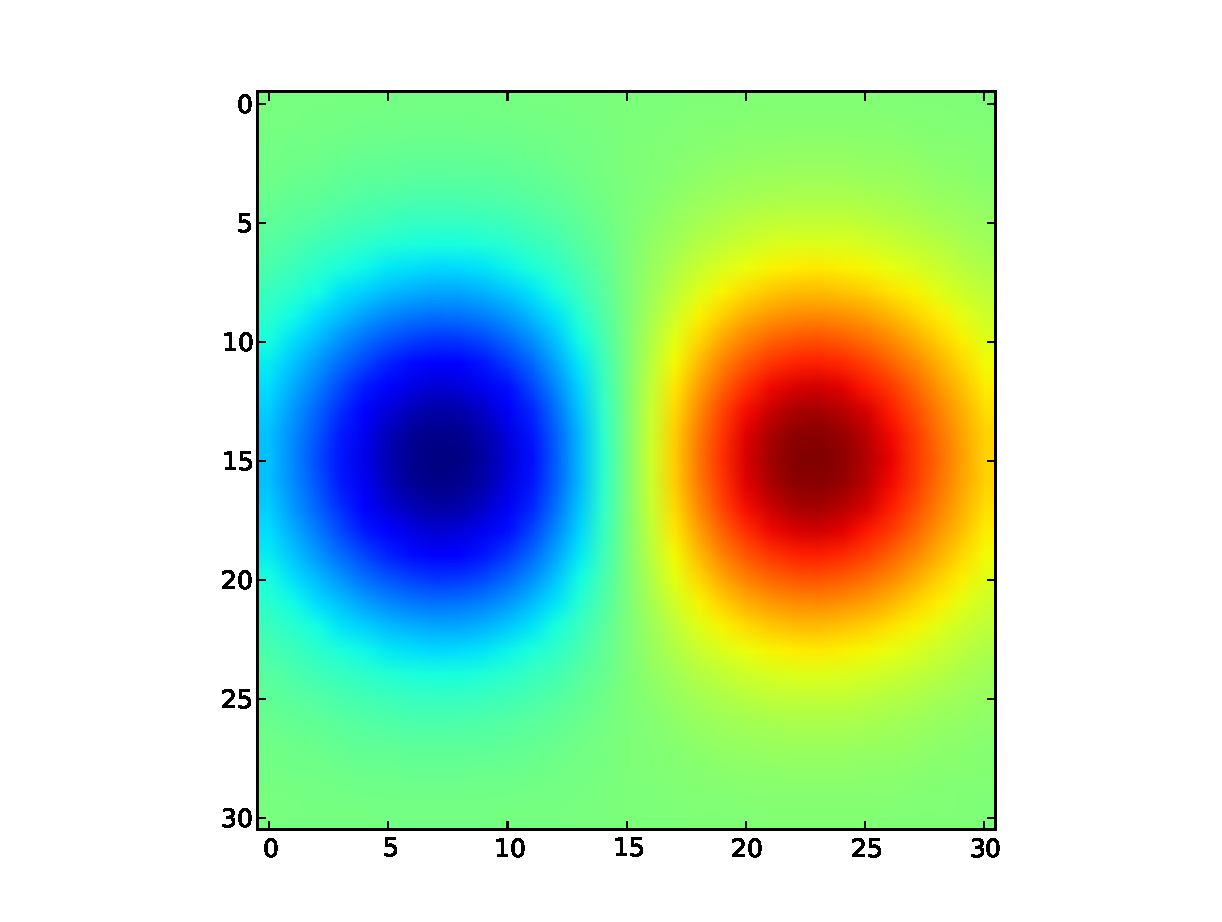
\includegraphics[width=\linewidth]{figs/bumps.pdf}
  \endminipage\hfill
  \minipage{0.5\textwidth}
    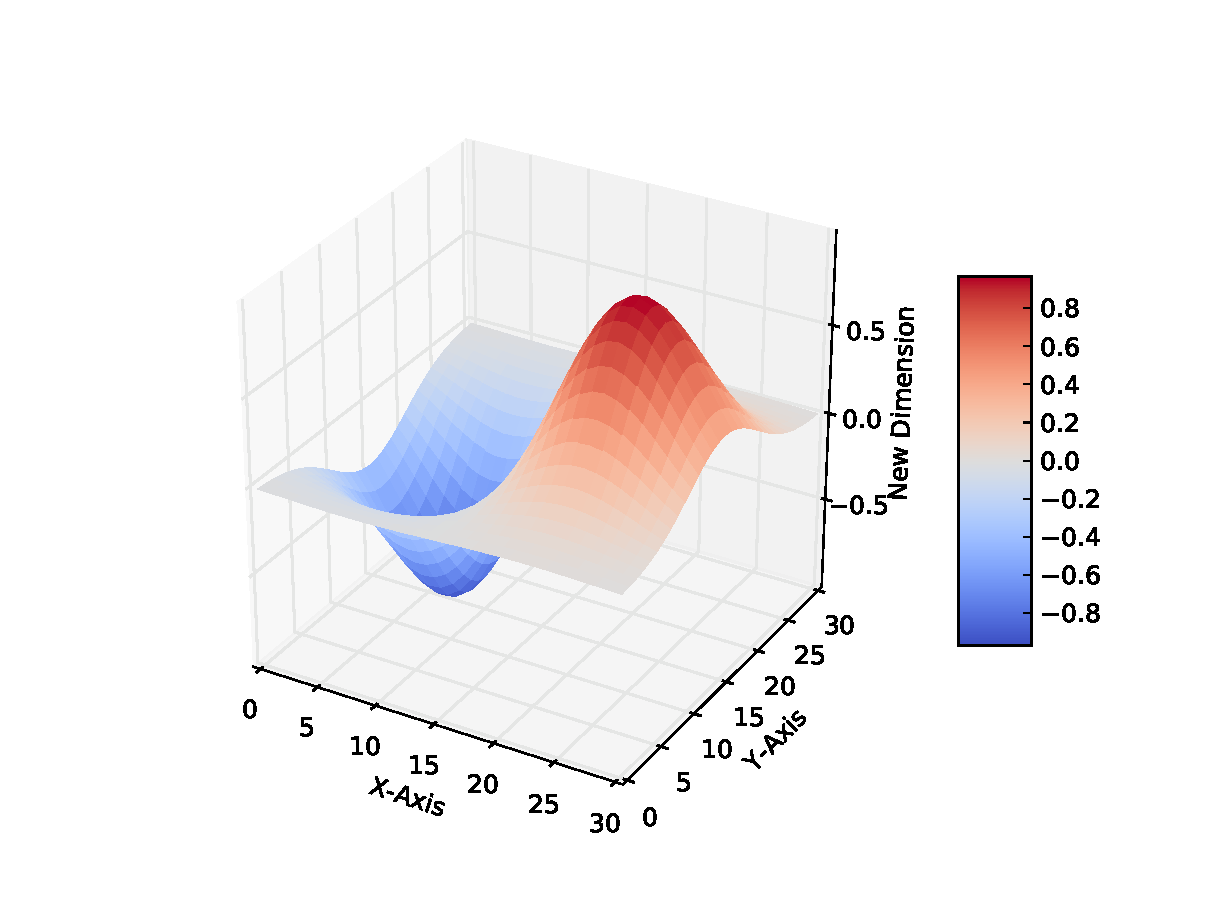
\includegraphics[width=\linewidth]{figs/tfbumps.pdf}
  \endminipage
\caption[Dimension-Adding WIT example]
{The figure on the left is a heatmap of some function.
The areas in red are where it attains a high value and the ones in blue
are where it attains a low value.
The figure on the right shows the transformed domain of the function.
The red areas are pulled up and out of the page while the blue ones are pushed
down and into the page. The areas where the domain is stretched most are
where the function has the steepest slope.}
\end{figure}

This transform does what we want, but it has two problems.
The first problem is that it is sensitive to the scale of $f$.
The fix is to normalize $f$ by its inverse target slope $\mu_f$; this way
$f$ has the same spread as its domain.
If we want to control the extent of the stretching, we can do so by also
scaling $f$ by a constant $\alpha$.
The second problem is that it is potentially diameter-increasing.
To counteract this, we should also normalize the new domain by 
a diameter-preserving constant, $c_0$.

With these changes, the $d$-dimensional vector, $x = (x_1, \ldots, x_d)$
gets mapped to $x' = c_0(x_1, \ldots, x_d, \alpha\mu_f\cdot f(x))$
The diameter-preserving $c_0$ is the ratio of the diameter of $X$ to the
diameter of the new space;
it satisfies  $\frac{1}{\sqrt{1+\alpha^2}} \leq c_0 \leq 1$.
Calculating $c_0$ exactly is difficult, so we just assume the lower
bound.
Note that this can potentially decrease the diameter, increasing the effective
bandwidth.

\begin{algorithm}
\caption{Dimension-Adding WIT}\label{dawitalg}
\begin{algorithmic}[1]
\Procedure{DAWIT}{$\tilde f$}
	\State $c_0 \gets \frac{1}{\sqrt{1+\alpha^2}}$
	\State\textbf{return}
          $x\mapsto c_0(x | (\alpha\mu_f\cdot\tilde f(x)))$
\EndProcedure
\end{algorithmic}
\end{algorithm}

To get a feel for what this transformer does, let us apply it to a concrete
example.
Assume the initial domain, $X$, is the unit interval $[0,1]$ and $f$ is a
function with range $[0,1]$ (so $\mu_f = 1$).
Calling \textit{DAWIT} on $f$ with $\alpha = 1.0$ will produce the
transform $x \mapsto \frac{1}{\sqrt{2}}(x, f(x))$.
This maps the unit interval to a curve in two dimensions.
Note that the maximum possible distance between points on this curve is $1$,
so the transform has not increased the diameter.
If we define a new function of two variables $f_2(x,y) = f(x)$ and call
 \textit{DAWIT} on it,
$X$ will be transformed into a curve in 3 dimensions; its points would take
the form $(\frac{x}{2}, \frac{f(x)}{2}, \frac{f(x)}{\sqrt{2}})$.
This curve can be rotated back into two dimensions to get the transform
$x \mapsto (\frac{x}{2}, \frac{\sqrt{3}}{2}f(x))$.
Calling \textit{DAWIT} in a loop $k$ times like this will transform the
domain to a $k+1$ dimensional curve which can be rotated to
$x \mapsto (\frac{x}{\sqrt{2^k}}, \sqrt{1-\frac{1}{2^k}}f(x))$.
Note how the domain is converging to a line---and not just any line.
It is converging to the best possible transform identified in the previous
chapter.
Since on every iteration, $x$ gets divided by $\sqrt{2}$,
this convergence happens exponentially quickly.
This happens for any connected $X$ and continuous $f$.

Now, let us see what happens when we run FIIRA with this transformer and
a kernel smoother.

\section{FIIRA with \textit{DAWIT} and a kernel smoother}
This section provides a discussion of the properties of the fit
generated when performing FIIRA with \textit{DAWIT} as the transformer and
a kernel smoother as the regressor.
For compactness, FIIRA with \textit{DAWIT} and a kernel smoother is referred
to as FDK.

\begin{claim} In the limit of infinite data and a bandwidth that shrinks at an
admissible\footnote{With admissibility as defined by Ormoneit et. al.
\cite{kbrl}} rate,
performing FDK to convergence produces the Platonic transform of the domain.
\end{claim}
\begin{proof} (sketch) If the bandwidth is sufficiently small,
$\tilde f_i \approx f$ for all $i$ because the approximation will be unaffected
by the representation.
Therefore the process would be like calling \textit{DAWIT} with the same
function on every iteration, which, as we saw above, results in convergence
to the Platonic transform.
This result implies that FDK preserves the statistical consistence
guarantees of kernel smoothing.
\end{proof}

\begin{claim} For any choice of bandwidth, dataset, and $\alpha$, performing
FDK will converge.
\end{claim}

\begin{proof} (sketch) To see this, let us first characterize the fixed points of
\textit{DAWIT}. A fixed point is a function whose domain does not get
distorted by the transform.
Let $f$ be a function that gets passed to \textit{DAWIT} and let
$a$ and $b$ be points in its domain.
 After the transform, the distance between $a$ and $b$ becomes
 $$\|\Phi(a)- \Phi(b)\| = \frac{1}{\sqrt{1 + \alpha^2}}
\sqrt{\|a-b\|^2 + \alpha^2\mu_f^2\cdot(f(a) - f(b))^2}.$$

This equals $\|a-b\|$ if only if $\mu_f \cdot |f(a) - f(b)| = \|a-b\|$.
For this to hold for all $(a,b)$ pairs, $f$ must have the same
slope everywhere.
Note that this is only possible if the domain of $f$ is one dimensional.
It follows that the fixed points of FDK
are datasets $D$ which produce $\tilde f$ such that
$\frac{\|x - x'\|}{|\tilde f(x) - \tilde f(x')|} = \mu_{\tilde f}$
for all distinct pairs of points $(x, x')$ in the domain of $\tilde f$ such
that $x \neq x'$.

The fixed points are not unique;
there are multiple datasets $D$ that result in such a $\tilde f$. An
elementary one is a set with only two distinct elements in the domain
(see proof in Appendix A).
A more interesting one is a set where all the $x_i$ are co-linear,
sorted by value, and spaced apart in such a way that $\tilde f$
is a line on its domain.
The first example is a stable fixed point and the second is an unstable one.
If the bandwidth is small enough, there can be stable fixed points
with more than two distinct elements.
For instance, if the mother kernel has compact support and a bandwidth less
than $\frac{\mathrm{diam}(X)}{c}$ for some $c$, then there exists a stable
fixed points with $c$ atoms (see proof in Appendix A).

On the $j^{th}$ iteration of FDK, points in $D_{j-1}$ are moved closer
together if the slope of $\tilde f_j$ between them is lower than
$\mu_{\tilde f_j}$.
Points that get moved closer together are likely to have similar values
on the next iteration, meaning they will get brought even closer.
This suggests that the domain is collapsing to a finite number of atoms.
\end{proof}

The fact that the domain collapses to a finite number of atoms implies
that FDK will produce a piecewise flat approximation to $f$.
Points that get mapped to the same atom will have the same value in the
limiting fit $\tilde f_\infty$.
Since there are a finite number of atoms $\tilde f_\infty$ will only take
a finite number of values. 
For a concrete example of how this happens, see Figures 4-2, 4-3, and 4-4.

\begin{figure}[!!!ht]
  \centering
    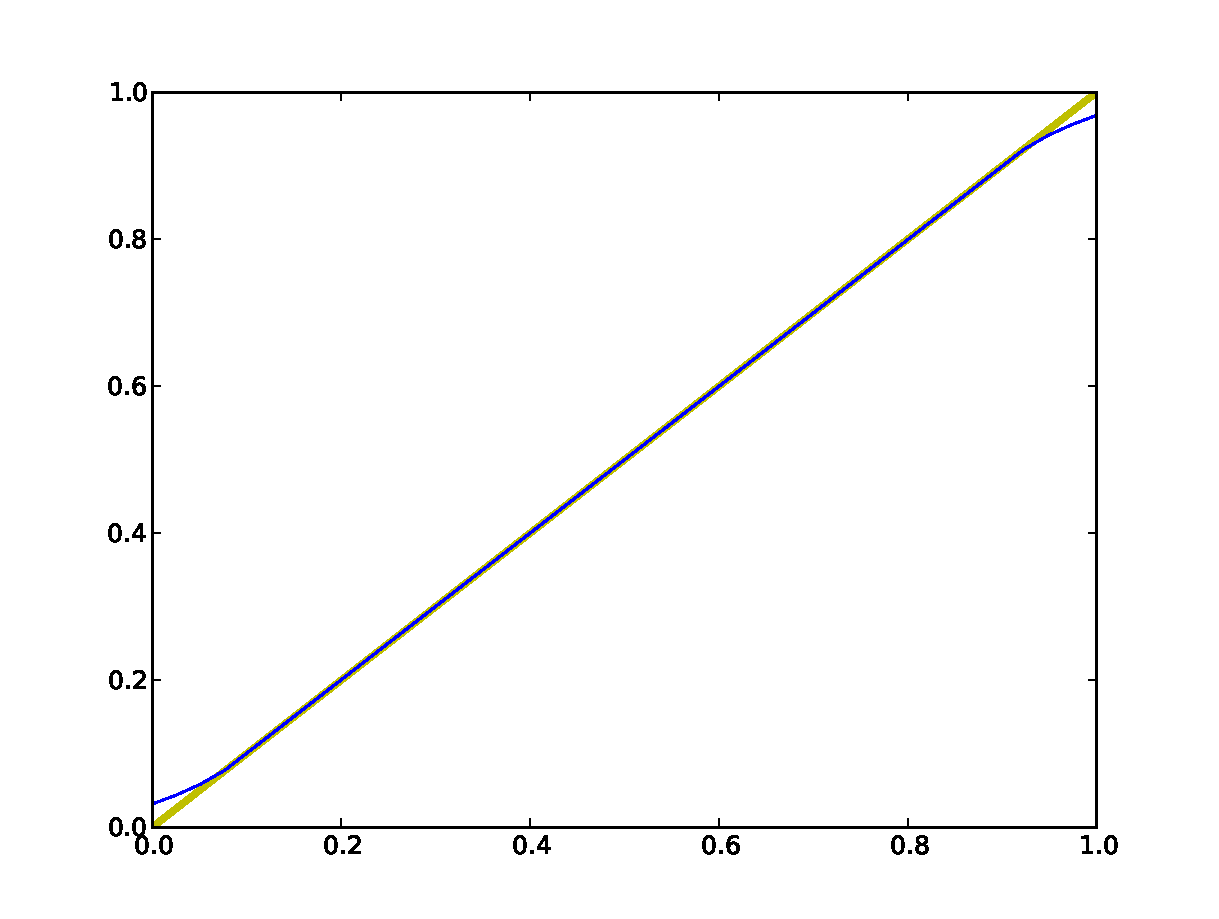
\includegraphics[width=80mm]{figs/linefit.pdf}
  \caption[Fitting a line with a kernel smoother]
  {The result of trying to fit a line with a local-averaging kernel
    smoother.
    Note how the fit is good in the interior but not at the boundaries.
    This is a well known flaw of kernel smoothers.}
  \label{fig:linefit}
\end{figure}

\begin{figure}[!!!ht]
  \centering
    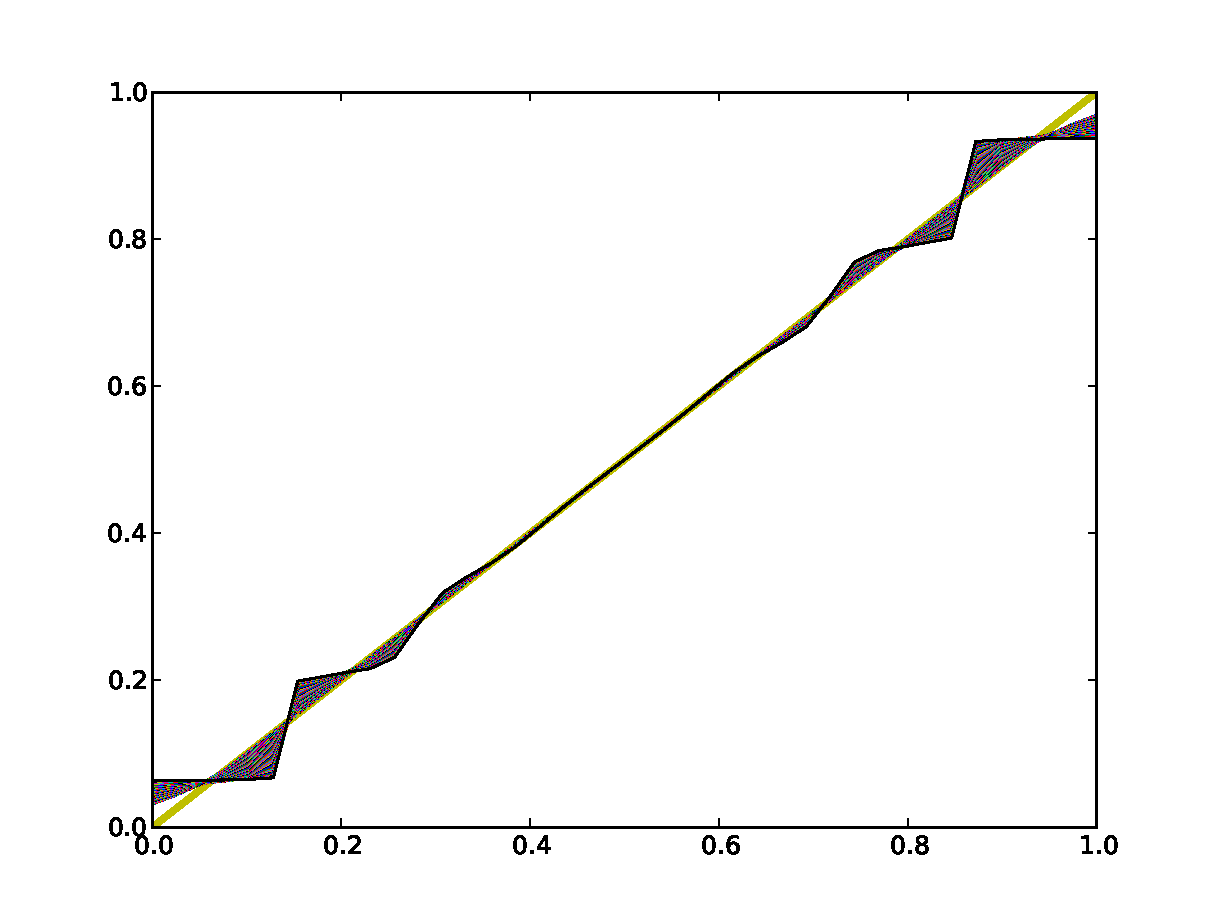
\includegraphics[width=80mm]{figs/linefitmid.pdf}
  \caption[Line fit error getting amplified]
  {In an effort to make $\tilde f$ linear, \textit{DAIWT} squashes
    the ends of the domain, amplifying the error and making the fit
	worse on successive iterations.}
  \label{fig:linefitmid}
\end{figure}

\begin{figure}[!!!ht]
  \centering
    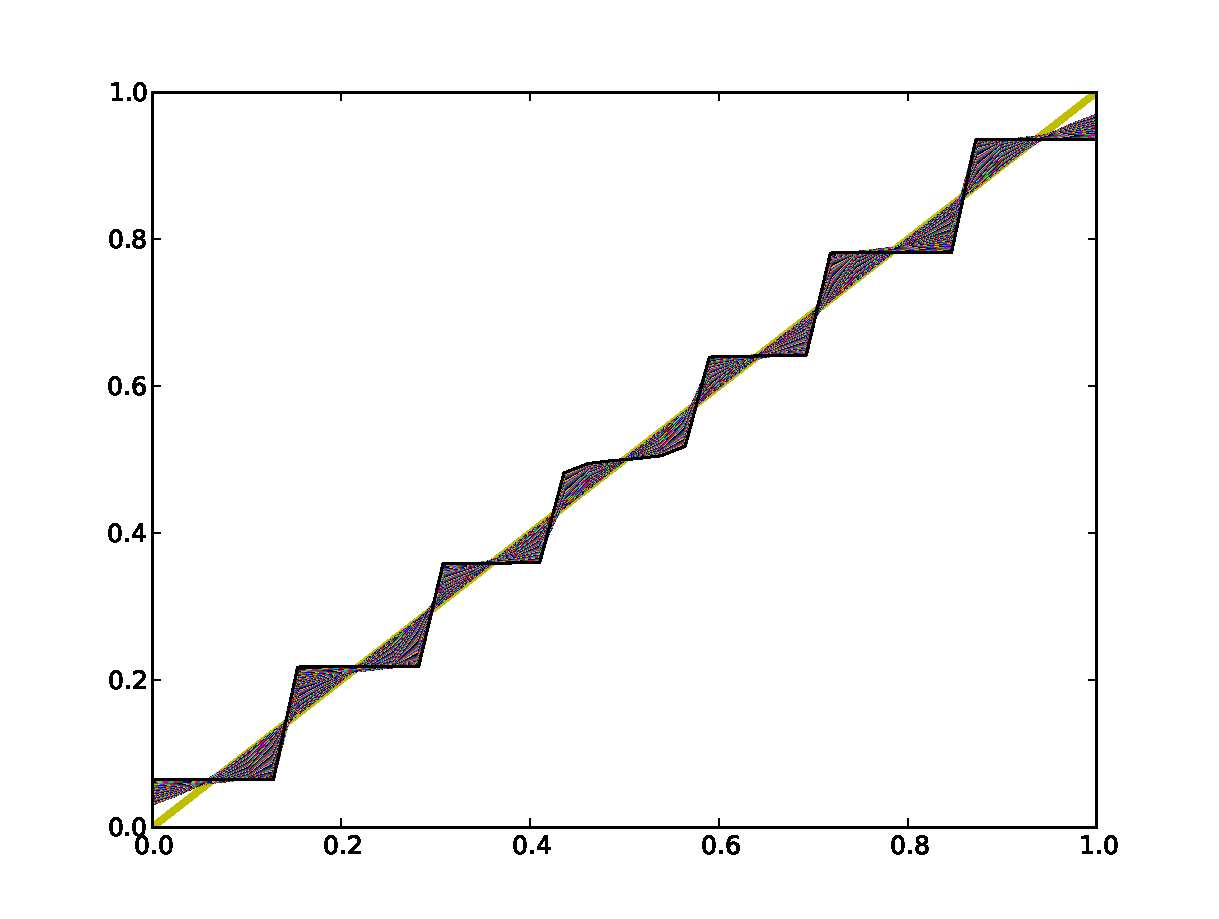
\includegraphics[width=80mm]{figs/linefitend.pdf}
  \caption[Fixed point of FIIRA]
{The process converges to a piecewise flat approximation.}
  \label{fig:linefitend}
\end{figure}

\begin{figure}[!!!ht]
  \centering
    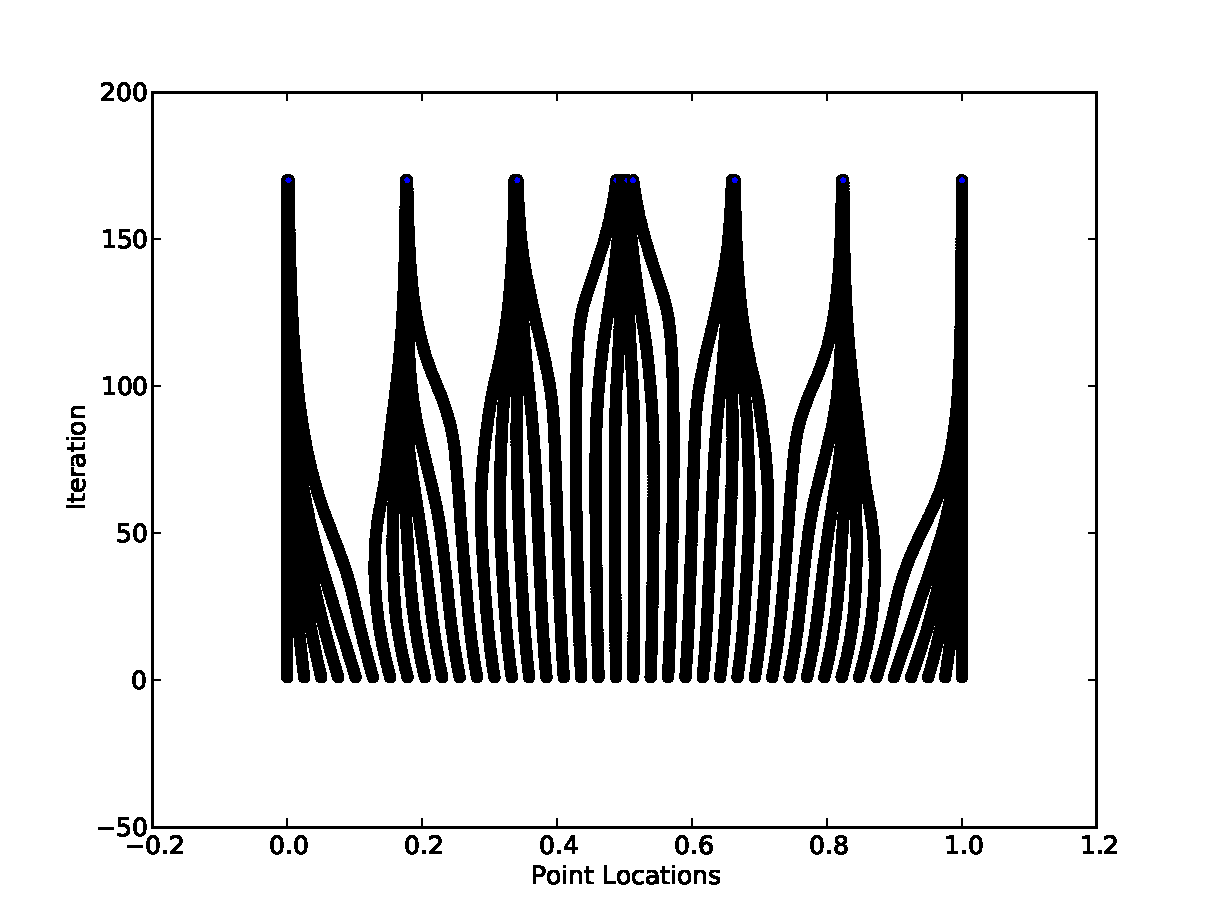
\includegraphics[width=100mm]{figs/linecon.pdf}
  \caption[FIIRA convergence]{How the domain collapses over time.
   First the points near the boundary move closer together,
   then the entire domain collapses to seven atoms.
   Had a smaller bandwidth been used, there would have been more atoms.}
  \label{fig:linecon}
\end{figure}

The reason FDK converges to a piecewise flat approximation is because
kernel smoothers make a local flatness assumption.
The inability of kernel smoothers to represent boundaries and curvature
well is a well-known problem.
A workaround is to use locally weighted regression instead of local
averaging \cite{kercar}.
Locally weighted regression would fix the bias at the boundaries and
just might prevent the piecewise flat convergence.
As noted Ormoneit \& Sen \cite{kbrl} KBRL can be modified to use regression,
but I do not explore that option in this thesis.

The fact that FDK converges to a piecewise flat approximation is not a
damning result.
For many functions, the fit gets better before it gets worse.
We merely stop the process when the best fit is obtained.
Figures 4-6 and beyond show the result when the algorithm is applied to 
a few different functions.

The plots on the left show the function being approximated (yellow), the kernel
smoother fit of the function (blue), the best FDK fit obtained (red), and the fixed
point function to which FDK converges for the value of $\alpha$
that produced the best fit (green).
The plots on the right show how the approximation error changes over
time for different values of $\alpha$.
Approximation error is measured as the sum of squared errors on the points
in the dataset used to generate the fits normalized so that the fit produced
by a the kernel smoother has unit error.

\begin{figure}[!htb]
  \minipage{0.5\textwidth}
    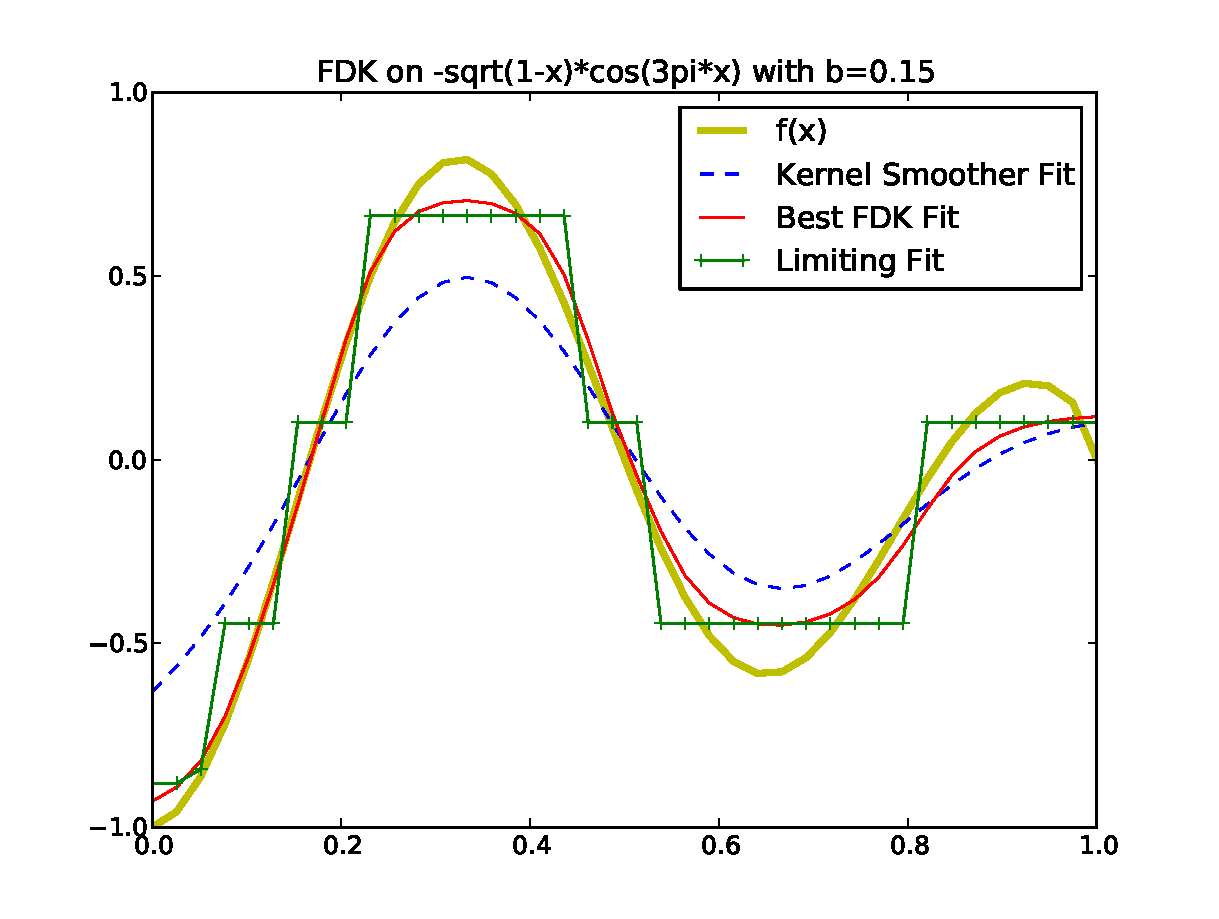
\includegraphics[width=\linewidth]{figs/chap4/sqcos.pdf}
  \endminipage\hfill
  \minipage{0.5\textwidth}
    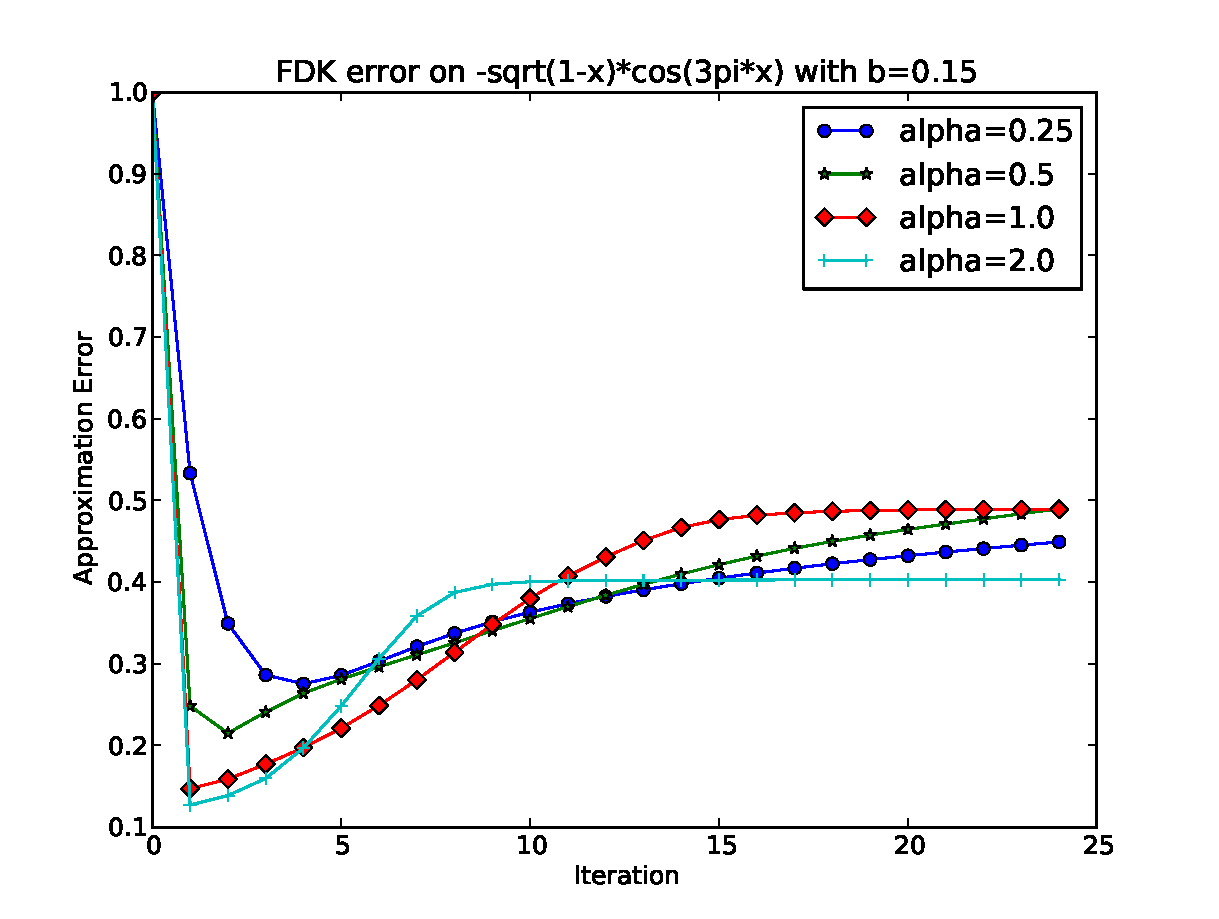
\includegraphics[width=\linewidth]{figs/chap4/sqcoserr.pdf}
  \endminipage
\caption[Fitting $-\sqrt{1-x}\cdot\mathrm{cos}(\pi x)$]
{FDK fit for $-\sqrt{1-x}\cdot\mathrm{cos}(\pi x)$.}
\end{figure}

\begin{figure}[!htb]
  \minipage{0.5\textwidth}
    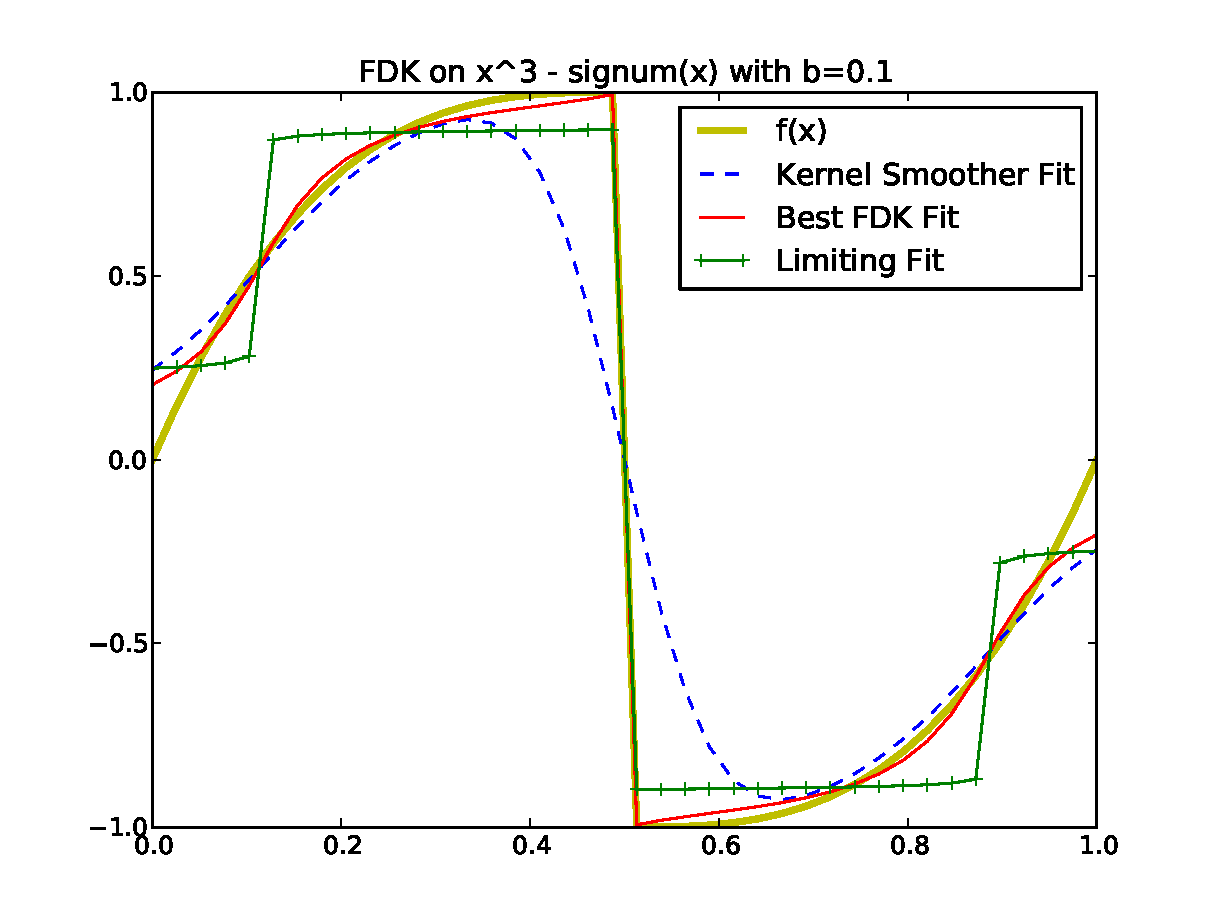
\includegraphics[width=\linewidth]{figs/chap4/flip.pdf}
  \endminipage\hfill
  \minipage{0.5\textwidth}
    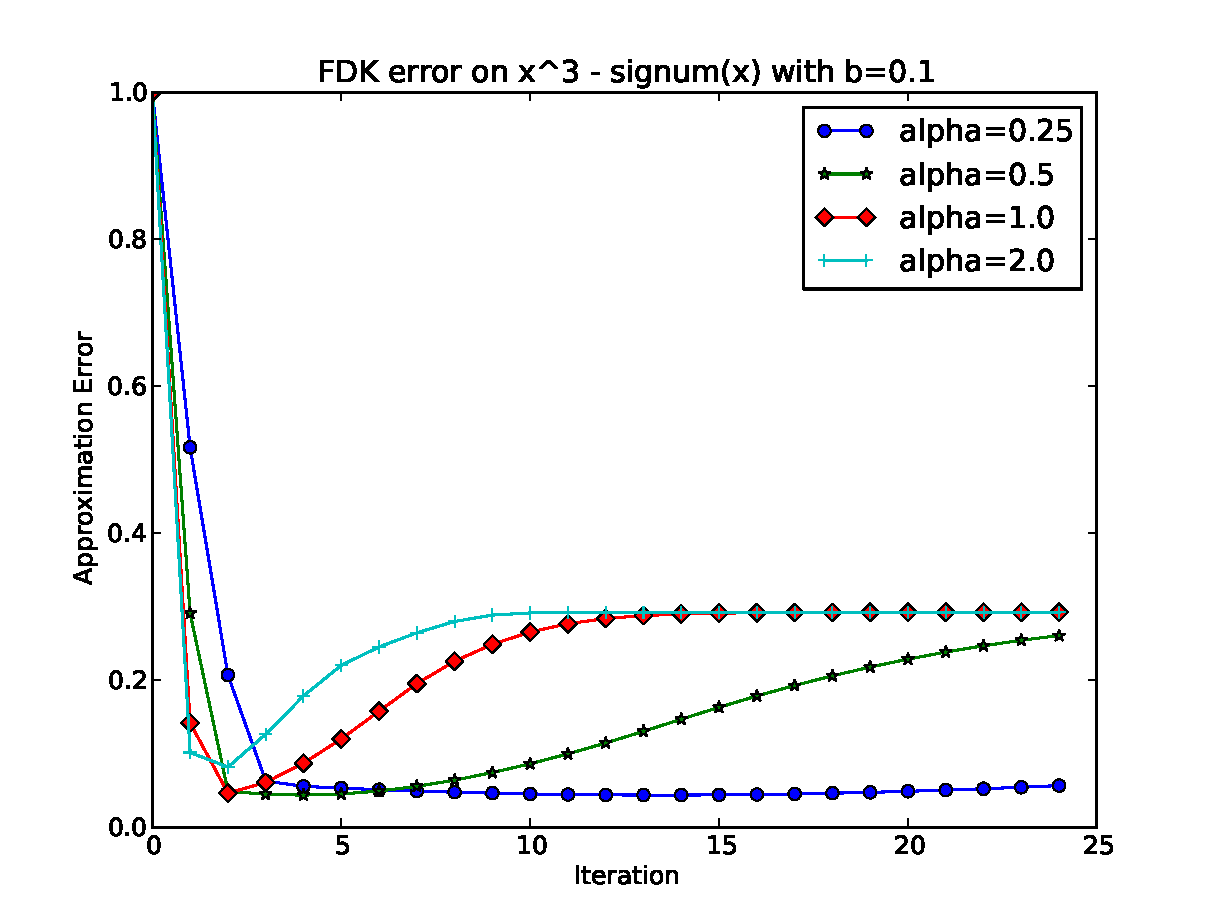
\includegraphics[width=\linewidth]{figs/chap4/fliperr.pdf}
  \endminipage
\caption[Fitting $x^3 - \mathrm{signum}(x)$]
{The same as above but here the function is $x^3 - \mathrm{signum}(x)$}
\end{figure}

\begin{figure}[!htb]
  \minipage{0.5\textwidth}
    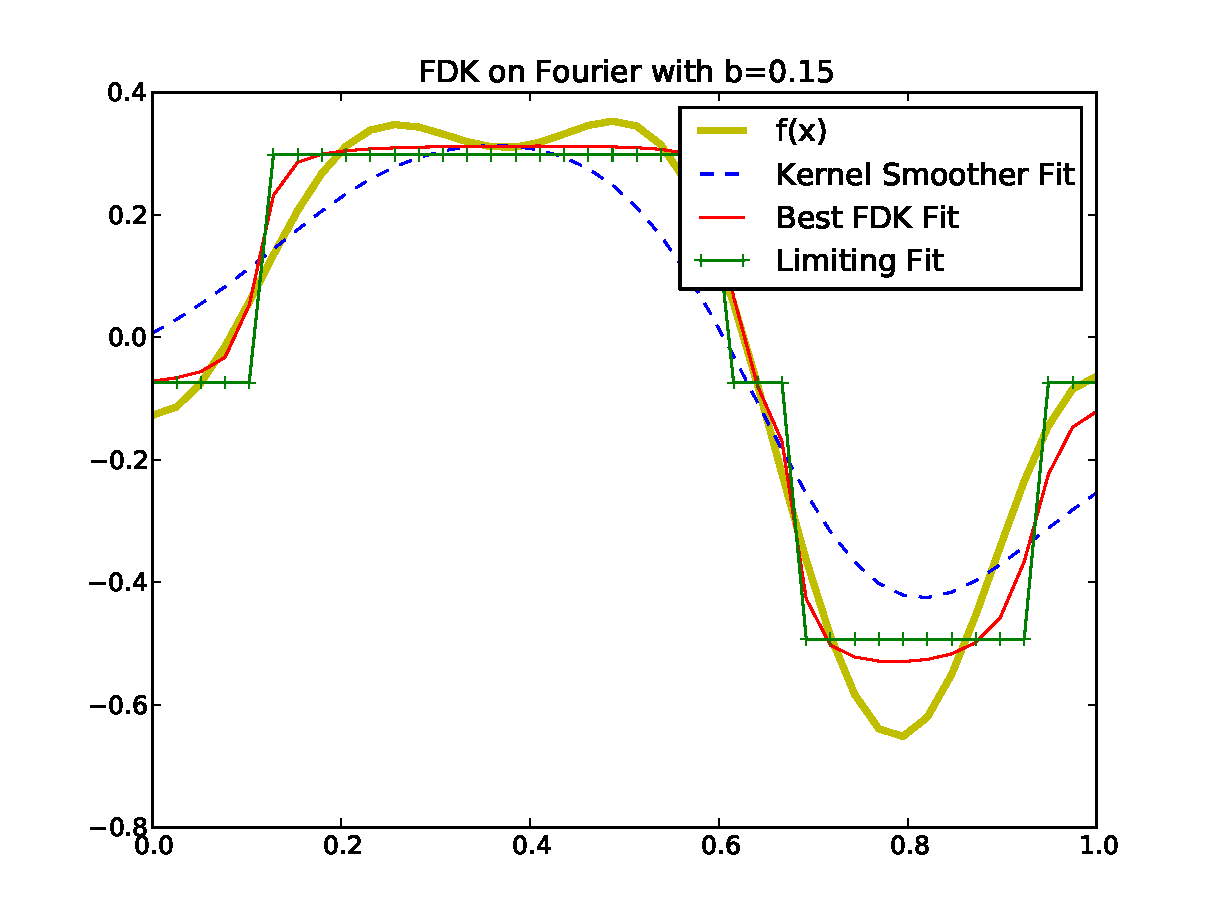
\includegraphics[width=\linewidth]{figs/chap4/bump15.pdf}
  \endminipage\hfill
  \minipage{0.5\textwidth}
    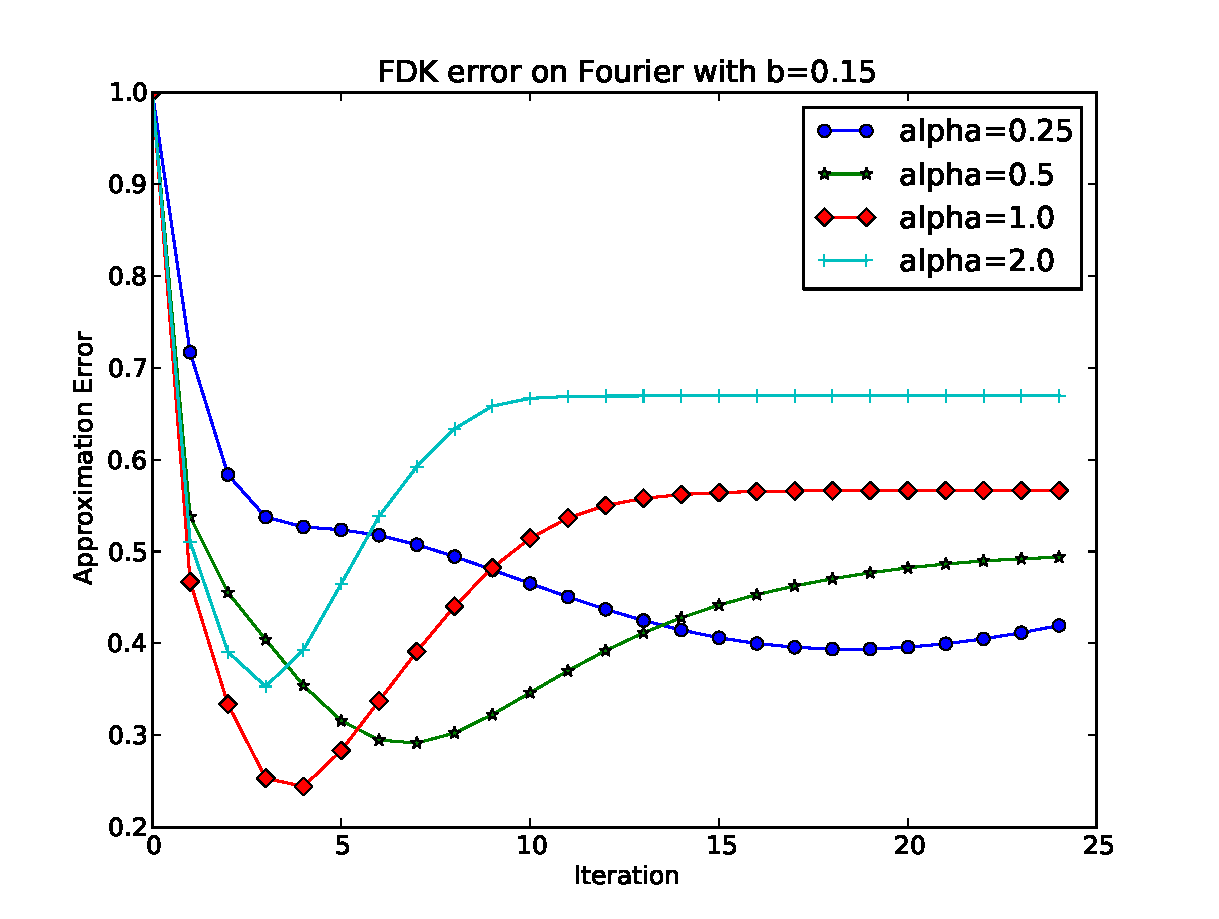
\includegraphics[width=\linewidth]{figs/chap4/bump15err.pdf}
  \endminipage
\caption[Fitting an order 5 Fourier function with $b = .15$]
{The same as above but here the function is some order 5 Fourier.}
\end{figure}


\begin{figure}[!htb]
  \minipage{0.5\textwidth}
    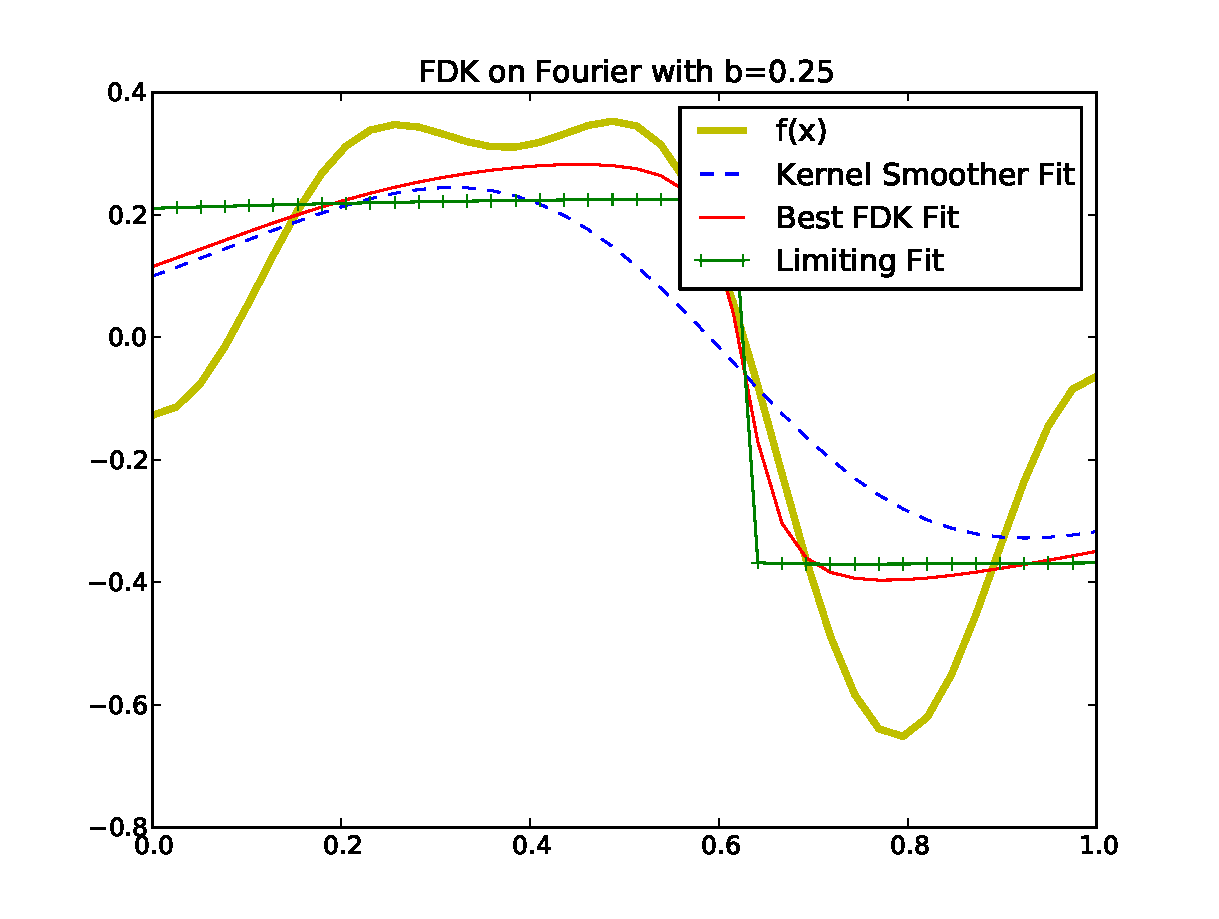
\includegraphics[width=\linewidth]{figs/chap4/bump25.pdf}
  \endminipage\hfill
  \minipage{0.5\textwidth}
    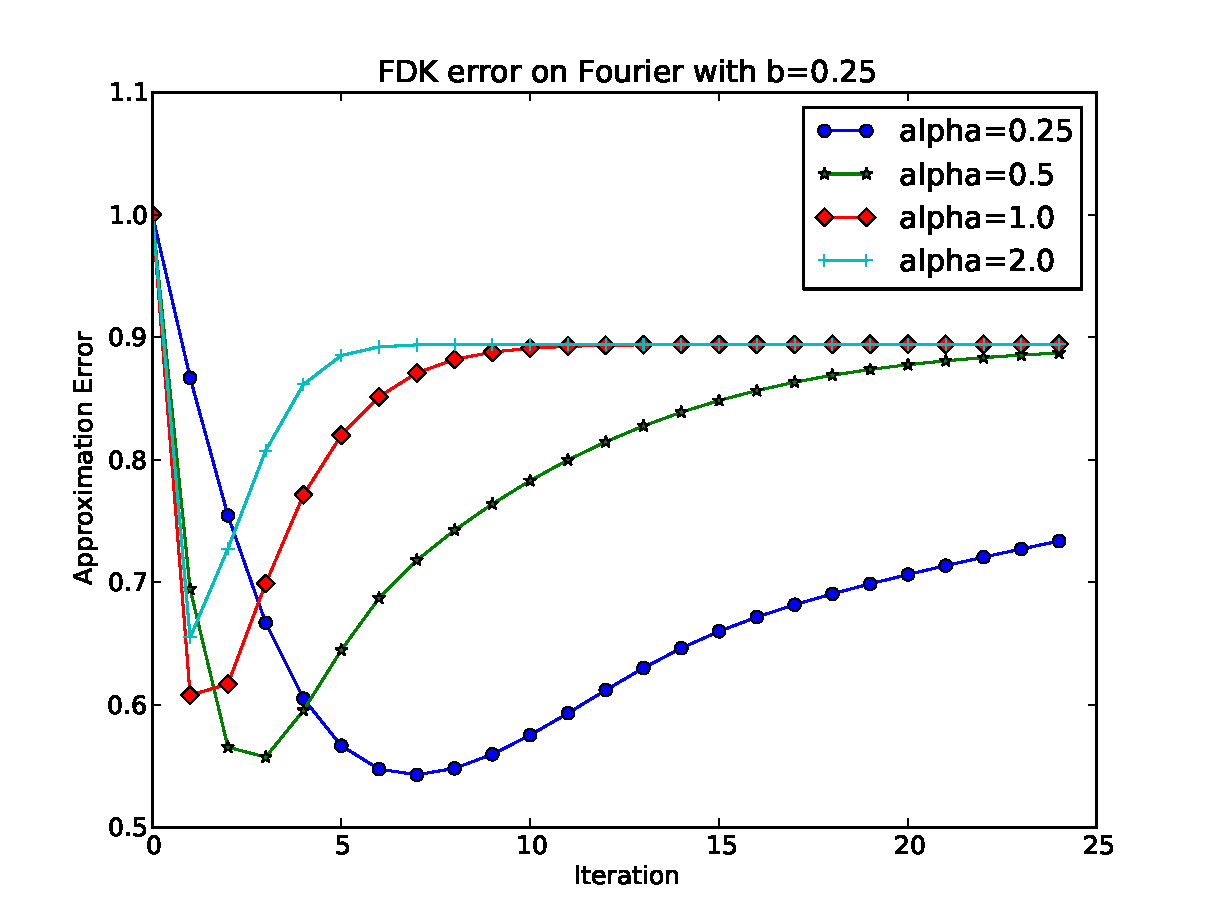
\includegraphics[width=\linewidth]{figs/chap4/bump25err.pdf}
  \endminipage
\caption[Fitting an order 5 Fourier function with $b = .25$]
{The same function as above, this time fit with a different bandwidth.}
\end{figure}

\begin{figure}[!htb]
  \minipage{0.34\textwidth}
    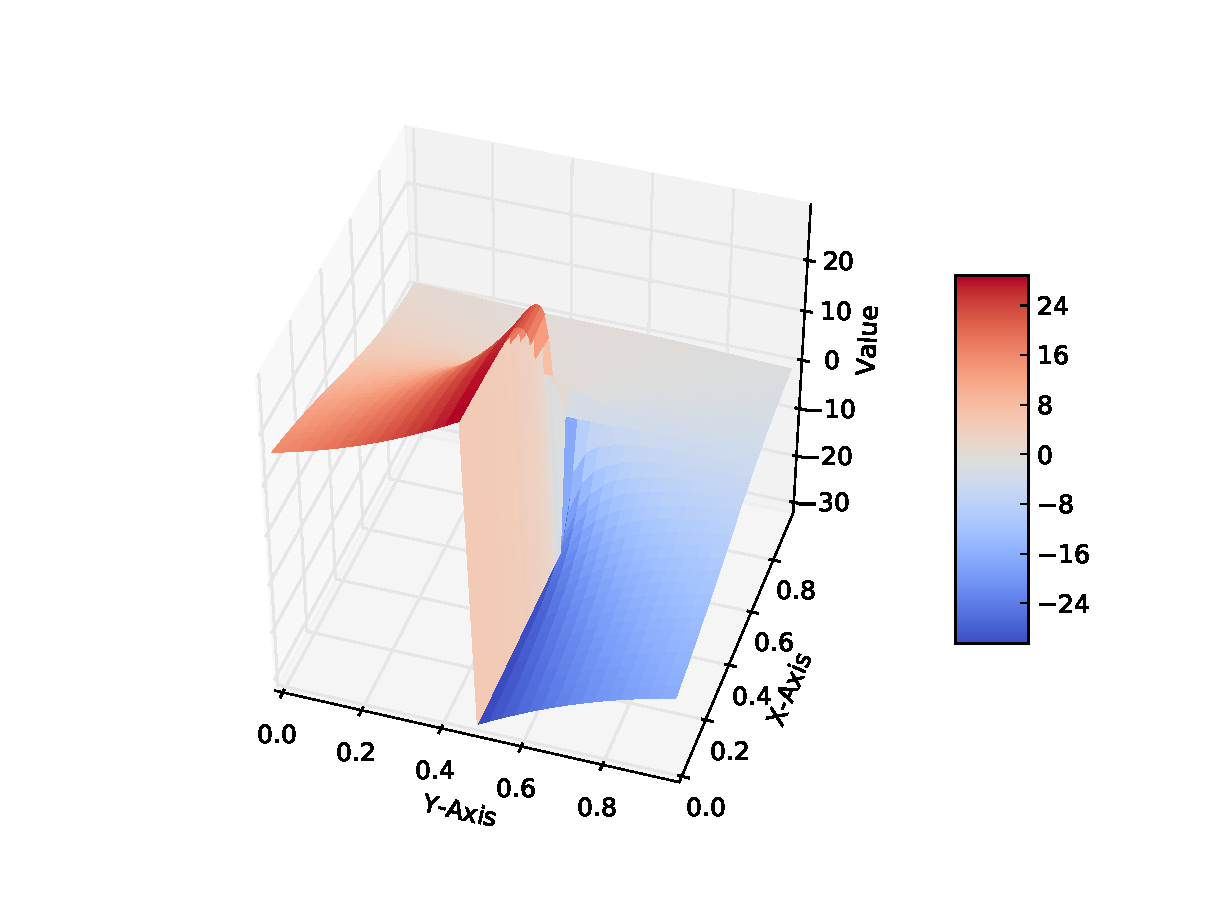
\includegraphics[width=\linewidth]{figs/chap4/atan.pdf}
  \endminipage\hfill
  \minipage{0.33\textwidth}
    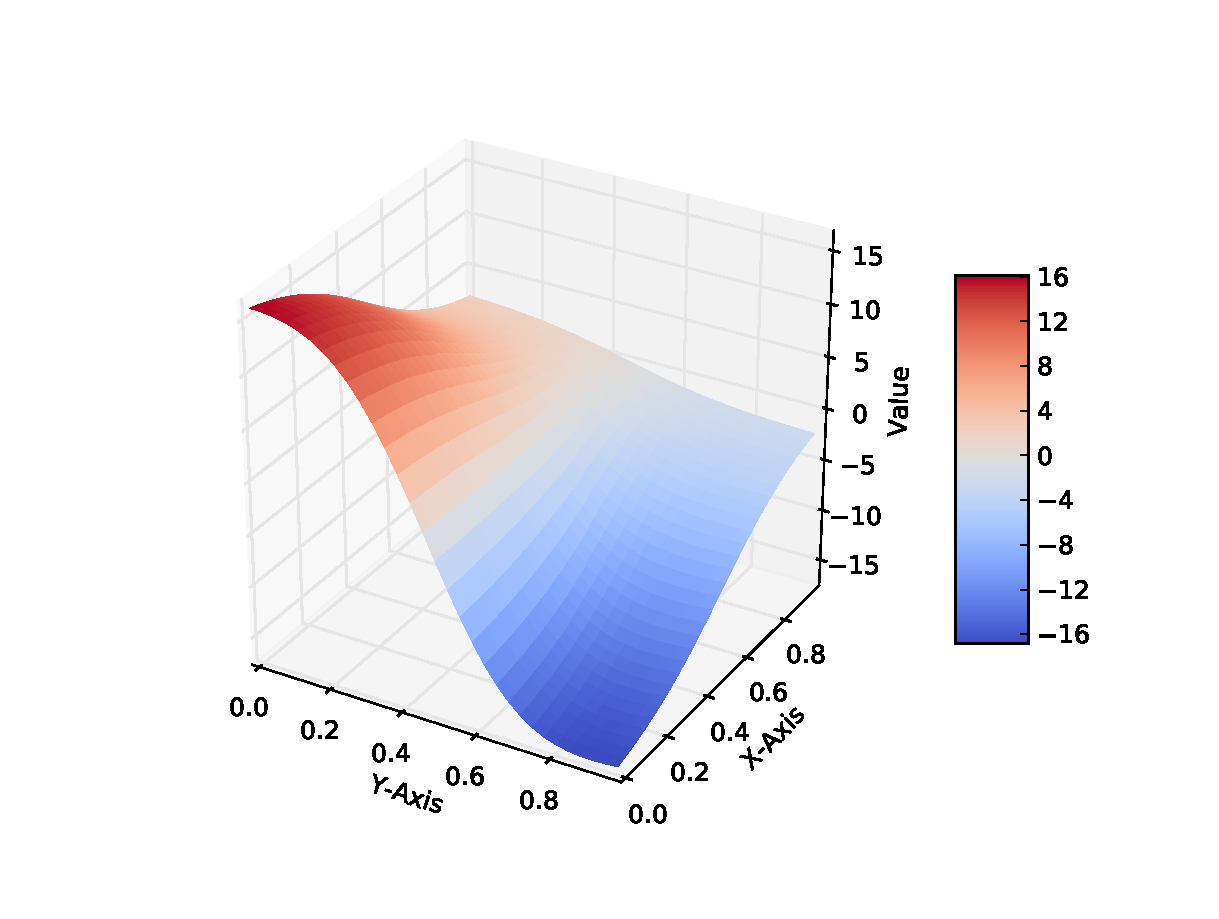
\includegraphics[width=\linewidth]{figs/chap4/atan3s.pdf}
  \endminipage
  \minipage{0.33\textwidth}
    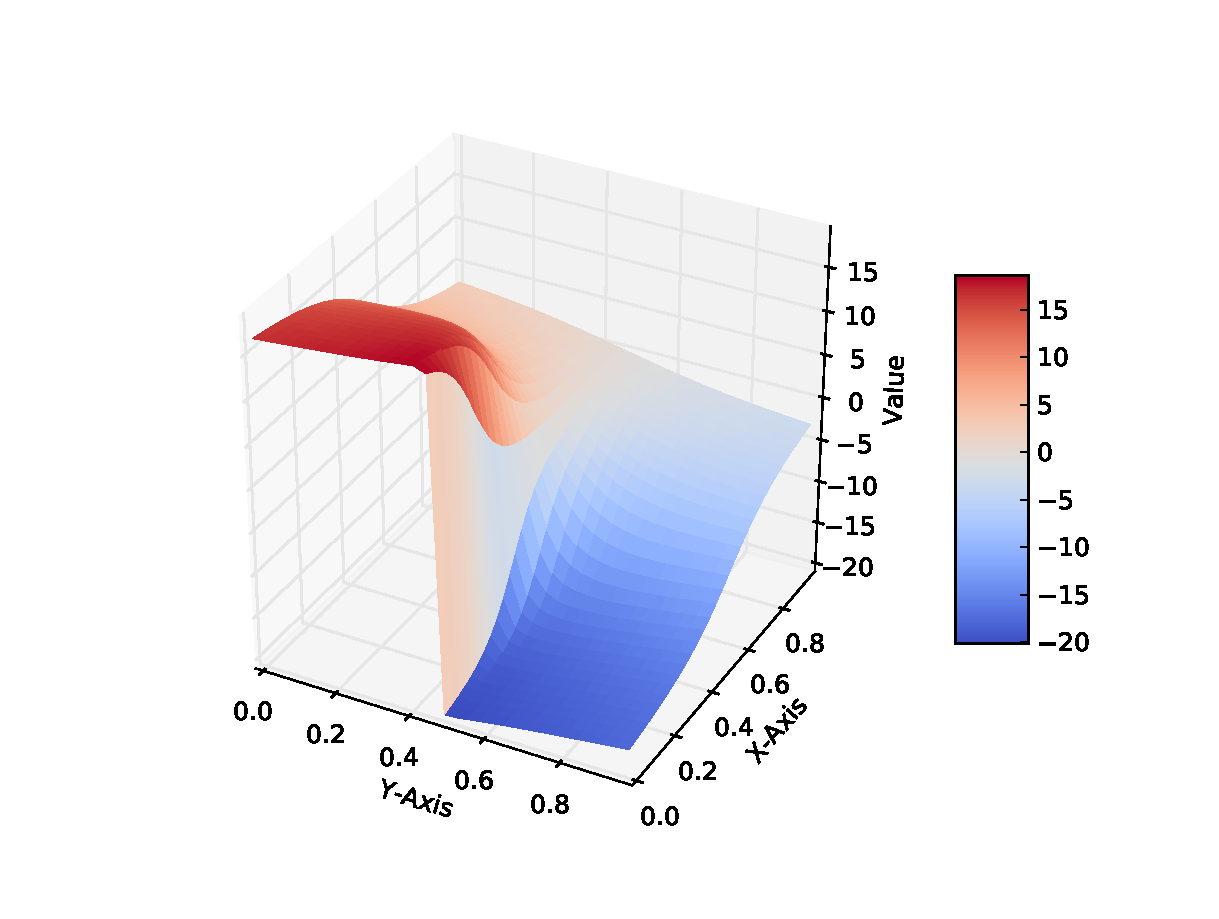
\includegraphics[width=\linewidth]{figs/chap4/atan3e.pdf}
  \endminipage
\caption[Fitting the arctan]{Fitting $f(x,y) = \tan^{-1}(x - .7, y - .5)^3$
Left is the function, mid is the kernel smoother fit, right is the FDK fit.}
\end{figure}

\begin{figure}[!!!ht]
  \centering
    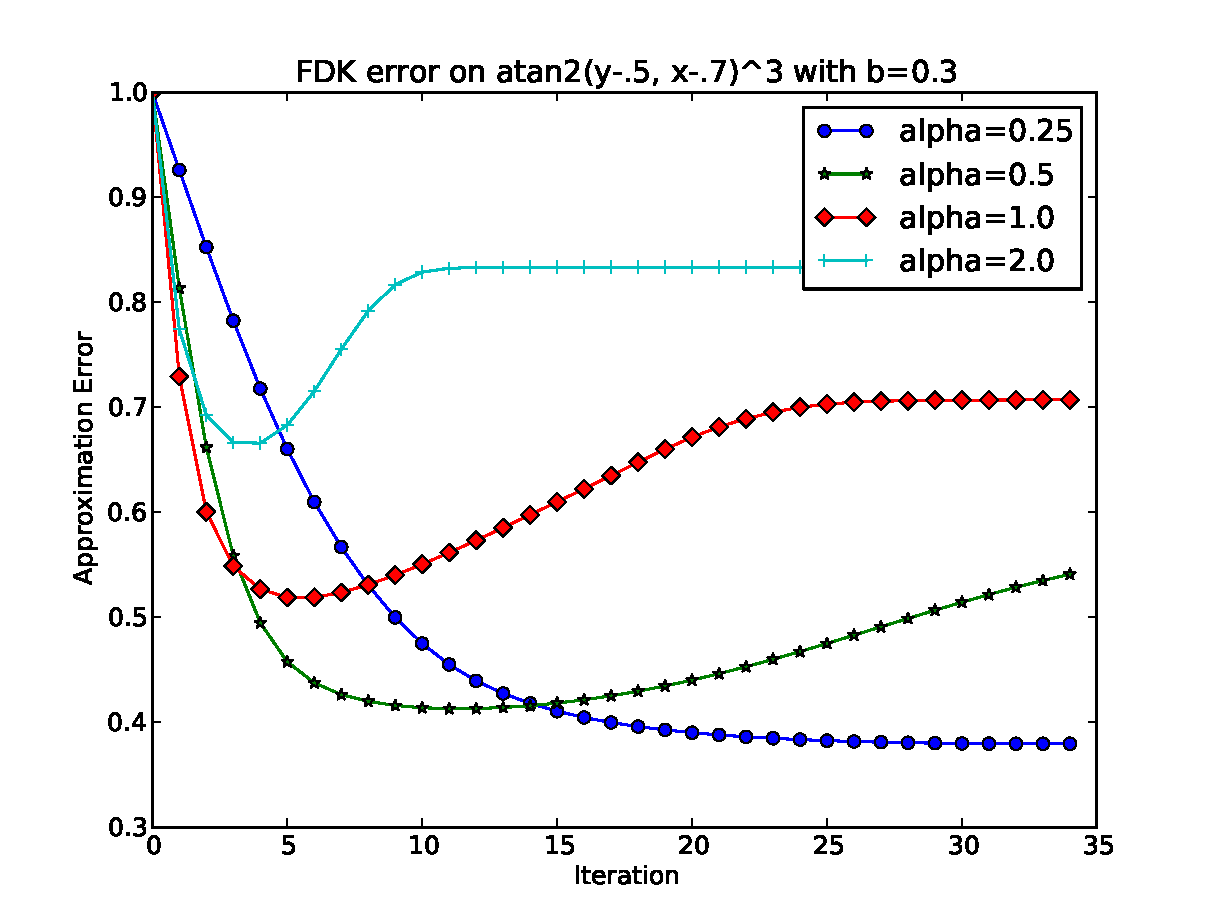
\includegraphics[width=80mm]{figs/chap4/atanerr.pdf}
  \caption{Approximation error when fitting the arctan function}
\end{figure}

These plots reveal several interesting properties of FDK.
First note how well FDK can represent functions with discontinuities.
Further note how few iterations it takes to reach the minimum-error
approximation.
Also note that the optimal value of $\alpha$ depends on the function being
approximated and the bandwidth being used.
Finally note that the error in the limit can depend on $\alpha$, this
means tha for different values of $\alpha$, FDK can collapse the domains to
different numbers of atoms.

\section{FIIRA approach to KBRL}
Algorithm 3 describes an FIIRA approach to KBRL.
Its inputs are the sample transitions, $S' = {S^a | a \in A}$, and
the bandwidth, $b$.

\begin{algorithm}
\caption{DAWIT-KBRL}\label{dkbrl}
\begin{algorithmic}[1]
\Procedure{DKBRL}{$S',\ b$}
	\State $\Phi^a_0 \gets x \mapsto x\ \forall a$
	\State $i \gets 0$
	\Repeat
		\State $Q_{i} \gets KBRL(S', b, \Phi_i)$
                \For{$a \in A$}
                    \State $\Phi^a_{i+1} \gets DAWIT(s \mapsto Q_{i}(s,a))$
                \EndFor
		\State $i \gets i+1$
	\Until{$Q_i \approx Q_{i-1}}$
           \Comment{Or until resulting policy stops improving.}
	\State \textbf{return} $Q_{i}$
\EndProcedure
\end{algorithmic}
\end{algorithm}

Note the following three points about line 5.\\
First, KBRL takes a transform as one of its inputs, this is assuming
KBRL has been modified to do all its local averaging in the transformed
space.\\
Second, The same set of sample transitions $S'$ is used on every
iteration of the algorithm.
One of the requirements for correctness in KBRL is that the data uniformly
cover the reachable state space.
To get the same correctness guarantees,
one would need to resample for coverage in the new space on every iteration.
Sampling for coverage in the new space is equivalent to concentrating samples
in the areas of the original space where the value function is steep.
In \textit{TWO-ROOM} this corresponds to drawing more samples near the
wall.\footnote{
In the analogy from Chapter 1, it corresponds to eating more bell peppers and
jalepe\~{n}os just to pinpoint the difference.}
This is a sensible thing to do because that is how one pinpoints the location
of the wall\\
Third, the regressor used does not have to be KBRL.
It could just as easily be KBSF or iKBSF.

We can see how DKBRL transforms the state space by trying it on
\textit{TWO-ROOM}. The figures show DKBRL discovering and opening up
the wall.

\begin{figure}[!htb]
  \minipage{0.34\textwidth}
    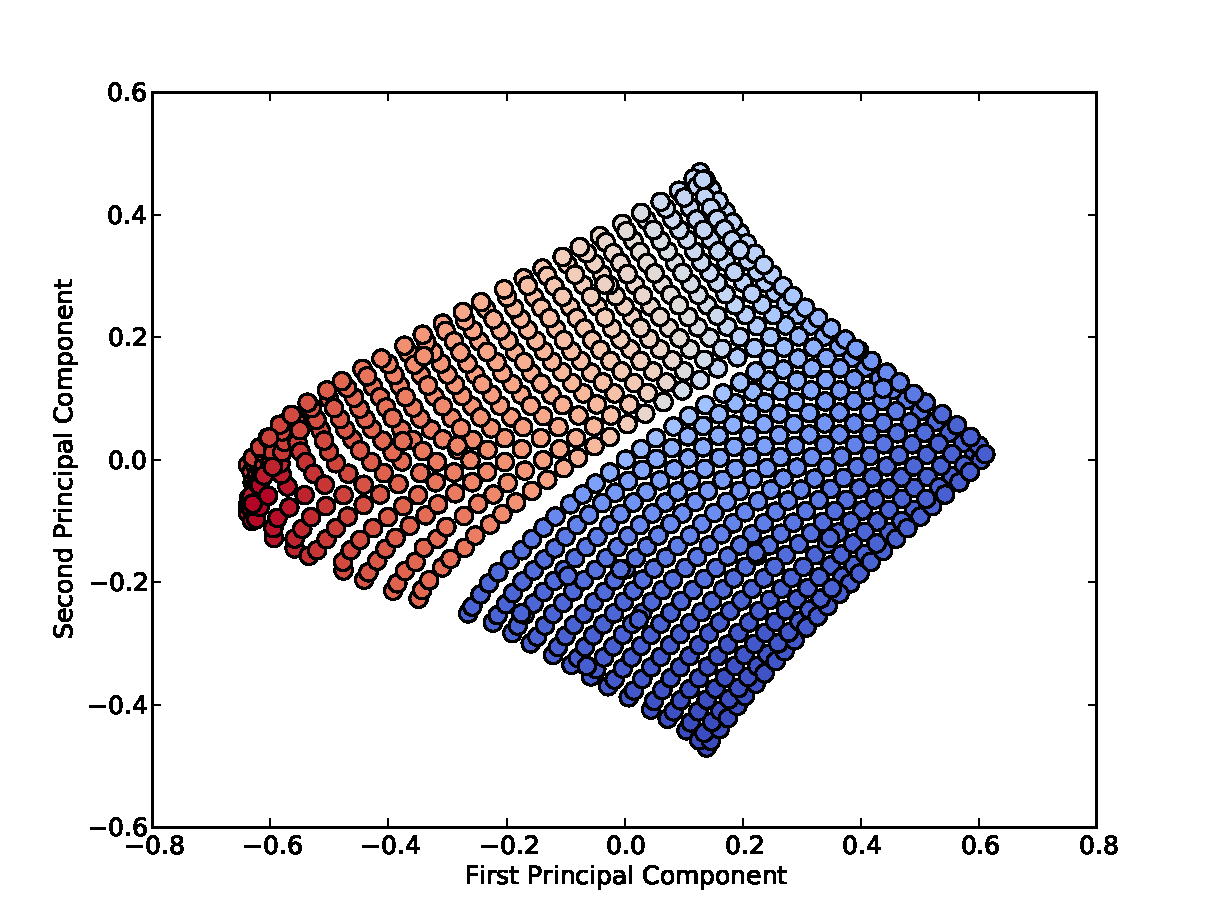
\includegraphics[width=\linewidth]{figs/chap4/2rmop1.pdf}
  \endminipage\hfill
  \minipage{0.33\textwidth}
    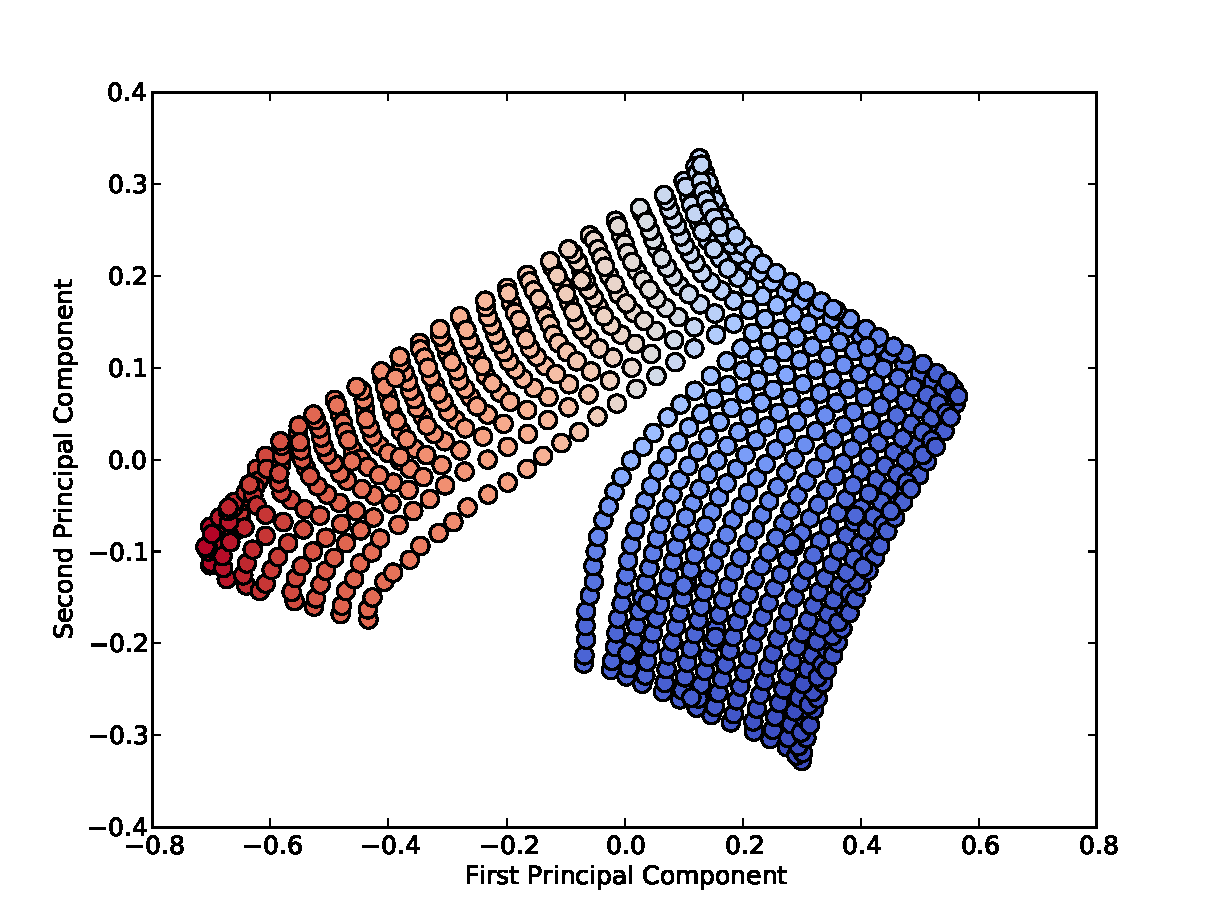
\includegraphics[width=\linewidth]{figs/chap4/2rmop2.pdf}
  \endminipage
  \minipage{0.33\textwidth}
    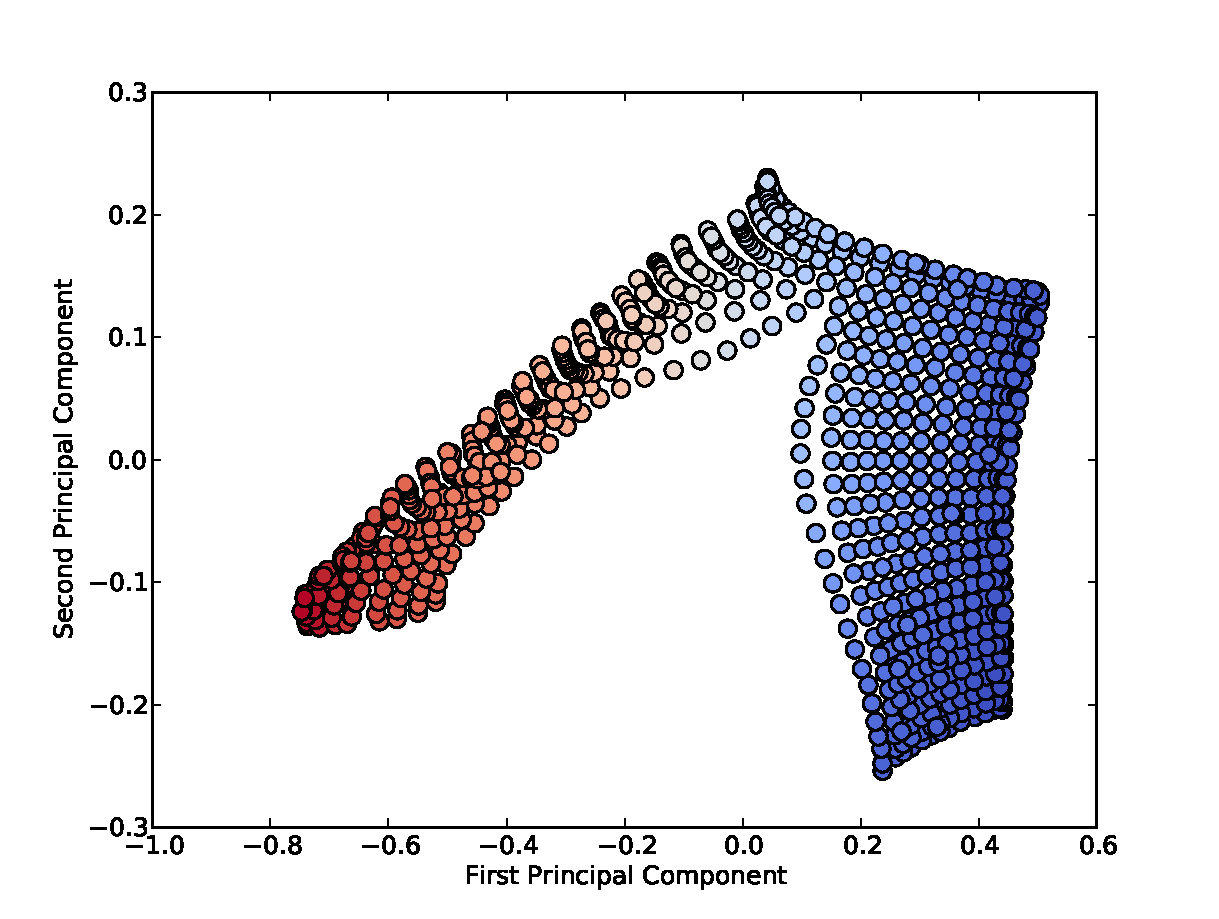
\includegraphics[width=\linewidth]{figs/chap4/2rmop3.pdf}
  \endminipage
\caption[DKBRL opening the wall in \textit{TWO-ROOM}]
{DKBRL opening the wall in \textit{TWO-ROOM} over three iterations.
The first iteration is on the left, it shows the algorithm has started pulling
points apart.
The third iteration is on the right, points are now completely separated by
value.
The points are coloured by their true value.
Note that this is a projection of the transformed space onto two dimensions.
This is why the red points look so squashed.
Along the third principal component (not shown) the red points do not
stack on top of each other as suggested by these pictures.}
\end{figure}

\begin{figure}[!!!ht]
  \centering
    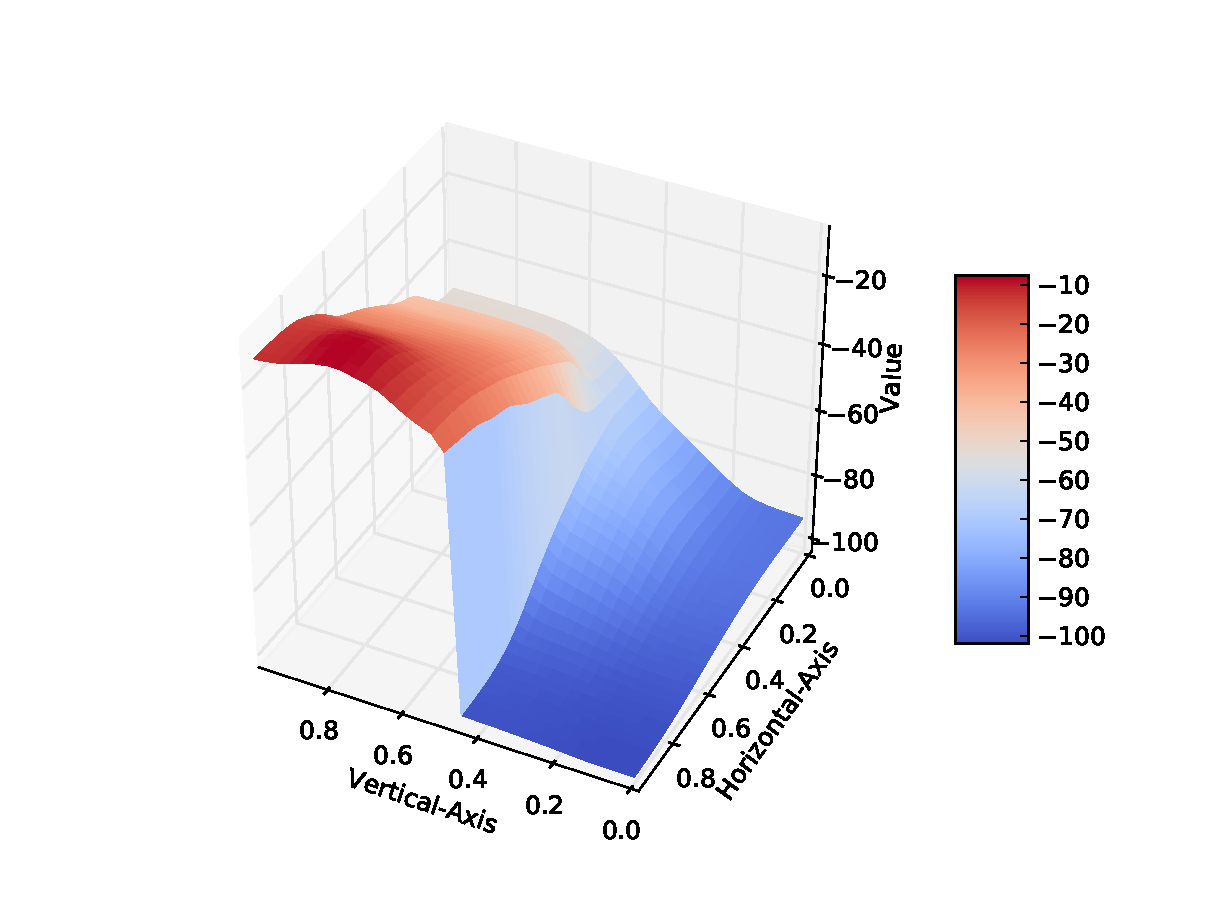
\includegraphics[width=110mm]{figs/chap4/2rmdkb.pdf}
  \caption[DKBRL fit for \textit{TWO-ROOM}]{The fit after three iterations
of KBRL. This was produced with a bandwidth of .06 and the same data as
in Figure 3-3.}
\end{figure}

\section{Implementation Considerations}
In the interest of clarity,
the algorithm descriptions above are not made efficient.
My implementations of these algorithms use the following optimizaions.

When KBRL performs value iteration on the finite model it constructs,
it uses the Q-Values from the previous iteration as a starting point.
This allows for the values to converge faster because the previous
Q-Values are likely to be close to the current ones.

Another optimization is that I do not explicitly compute a transform when
doing FIIRA with a kernel smoother.
Kernel smoothers only need an expression for the distance between points.
So one could do all calculations in terms of
$\mathrm{dist}_i(x_1 - x_2) = \|\Phi_i(x_1) - \Phi_i(x_2)\|$.
This distance can be calculated without $\Phi_i$ using the recursive equation

$$\mathrm{dist}_j(x_1, x_2) = \frac{1}{\sqrt{1 + \alpha^2}}
\sqrt{\mathrm{dist}_{j-1}(x_1, x_2)^2 + \alpha^2\mu_{\tilde f_j}^2
\cdot(\tilde f_j(x_1) - \tilde f_j(x_2))^2}.$$

Note that naively computing distances this way will take time exponential
in $j$, so doing this efficiently requires memoization.

A possible concern about adding dimensions is that it might make the
problem harder. Note that when the dimensions are added, the state space
retains its original dimensionality---it just becomes a manifold
in higher dimensional space.
The performance of kernel regression depends on the dimension of the manifold
and not the dimension of the embedding space.

As a final implementation consideration, note that the space created by the
transform can be visualized using MDS to rotate
the space so the principal components are axis aligned.

My implementations use all of these optimizations. The next chapter shows
the result of applying Algorithm 3 to some benchmark RL problems.

\chapter{Results}
This chapter evaluates the empirical performance of DKBRL and DKBSF.
It does this by comparing their performances with those of KBRL and KBSF
on the benchmark RL problems Mountain-Car, Acrobot, and Pinball.

\section{Experiment Design}
This section describes the way experiments were set up so anyone may
critique the methods or attempt to reproduce the results.
Since it would be impractical to enumerate all the relevant implementation
details, only the critically important points are mentioned.

\begin{description}

\item[Sampling Strategy]
I wanted to generate sample transitions whose start points 
uniformly cover the reachable part of the state space.
To generate reachable points,
I performed a random walk (selecting actions u.a.r. on every step) for $\approx10^6$
steps, starting from the start state and restarting whenever I reached the goal.
After generating these points, I subsampled the desired number of evenly spaced
points by clustering the points and taking the median of each cluster.

To reduce the correlation across datasets, I performed a separate random walk
for every time I needed a dataset.
Despite this, there is still correlation because the process of sampling for
coverage creates similar datasets.
Note that the sample transitions for the different actions all share the same set of
starts.
The plots that show ``number of samples'' below are all discussing the
number of sample transitions \textit{per action}.

\item[Domain Implementation]
My implementations of the three domains were each adapted from their
publicly available sources with some modifications.
First, I rescaled the domains to fill a unit cell.
Second, I refactored them to conform to my MDP solver's API.\footnote{
This mainly consisted of making the MDP instances immutable and renaming some
methods.}
Finally, I ended episodes where the agent failed to reach the goal after some 
number of steps $n_c$ ($500$ for Mountain-Car and Pinball, $1000$ for Acrobot).
When calculating average finishing time,
I treated the episodes where the agent failed to reach the goal as if the agent
reached the goal in $n_c$ steps.

\item[Learner Implementation]
I used my own implementations of KBRL and KBSF.
I implemented them as they were described in the papers introducing them
with three necessary modifications:
I implementated them to take a distance function as input and use that in
place of Euclidean distance for all kernel computations;
I modified KBRL so that the finite model it creates enforces the constraint
that terminal states self-transition with zero reward;
in the event of arithmetic underflow when performing local averaging,
I automatically take the value predicted by the nearest neighbour.

I used a Gaussian as my mother kernel in all experiments.
For the parts involving linear algebra, I used the matrix libraries
EJML\footnote{https://code.google.com/p/efficient-java-matrix-library/} and
Parallel Colt.\footnote{
https://sites.google.com/site/piotrwendykier/software/parallelcolt}

For DKBRL and DKBSF, I do not resample between iterations even though this
is necessary for maintaining the correctness guarantees of KBRL (as noted in
the previous chapter).
I decided against resampling because the added computational cost would
outweigh the potential improvement in solution quality.

\item[Parameters]
The purpose of these experiments is to demonstrate typical case performance,
not to show what happens with optimally chosen settings.
As a result I did not attempt to tune any parameters.
For most of these parameters, the value chosen affects KBRL/KBSF and
DKBRL/DKBSF identically.

For the bandwidths, I picked a range of bandwidths I expected would be
representative based my experiences when implementing the algorithms.
For $\alpha$, I chose $1$ in every test (except where stated otherwise) because
it was consistently adequate in the tests I performed for Chapter 4.
I capped the number of iterations of DKBRL at four; the experiments in
Chapter 4 suggest this would be sufficient.
For the sustained actions, I chose $\epsilon=.1$ ($0.15$ for Acrobot),
a number within an order of magnitude of the expected minimum distance between
points for sample densities used.
\end{description}
That covers all the important details about the experiment design.
We now proceed to the results.

\section{Mountain-Car}
Mountain-Car is a two dimensional MDP described by Sutton and Barto
\cite{rlai}.
The code was adapted from RL-Glue \cite{rlglue} .
Mountain-Car is meant to simulate a car with a weak motor attempting to
drive out of a valley.
The car is not powerful enough to escape directly and must build up
energy by swing back and forth.
The two dimensions correspond to the car's position and its velocity.
The car has three actions: REVERSE, NEUTRAL, and FORWARD.
The optimal trajectory out of the valley is 102 steps long.

\begin{figure}[!!!ht]
  \centering
    \includegraphics[width=90mm]{figs/mcexpl.png}
  \caption[Mountain-Car domain]{Picture of the Mountain-Car domain
(taken from rl-community.org, available under GNU Free Documentation Licence)}
\end{figure}

Despite its simplicity, Mountain-Car is an interesting domain that
illustrates some key properties of DKBRL.
Mountain-Car's value function has a discontinuity that spirals through the
state space (See Figure 5-2).
This spiral separates points where the car has enough energy to make it up
the hill on its current swing from points where the car needs to make an
extra swing.
The spiral occurs in slightly different positions in the Q-Values of the three
actions.
A good transform is one that unrolls the space along the spiral.

\begin{figure}[!htb]
  \minipage{0.5\textwidth}
    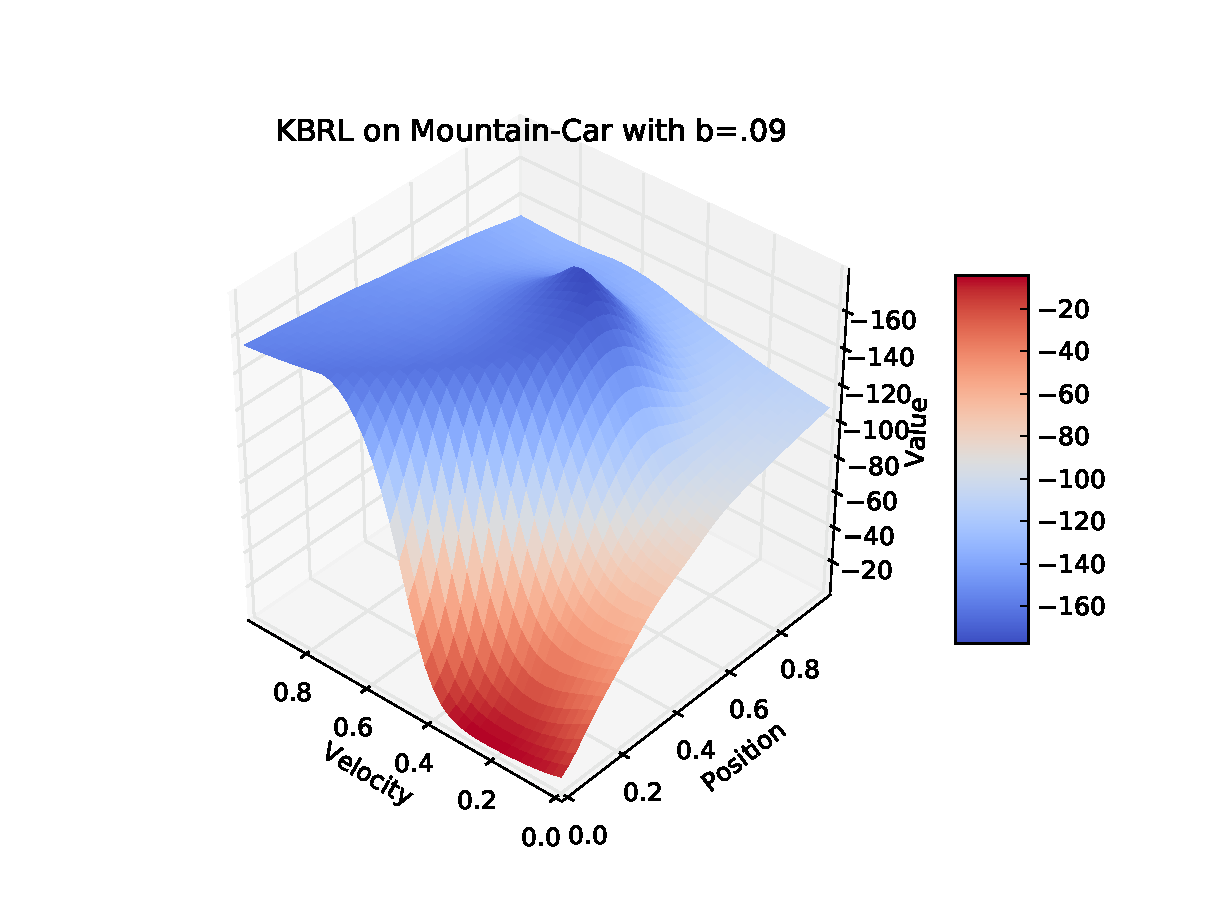
\includegraphics[width=\linewidth]{figs/chap5/mc09first.pdf}
  \endminipage\hfill
  \minipage{0.5\textwidth}
    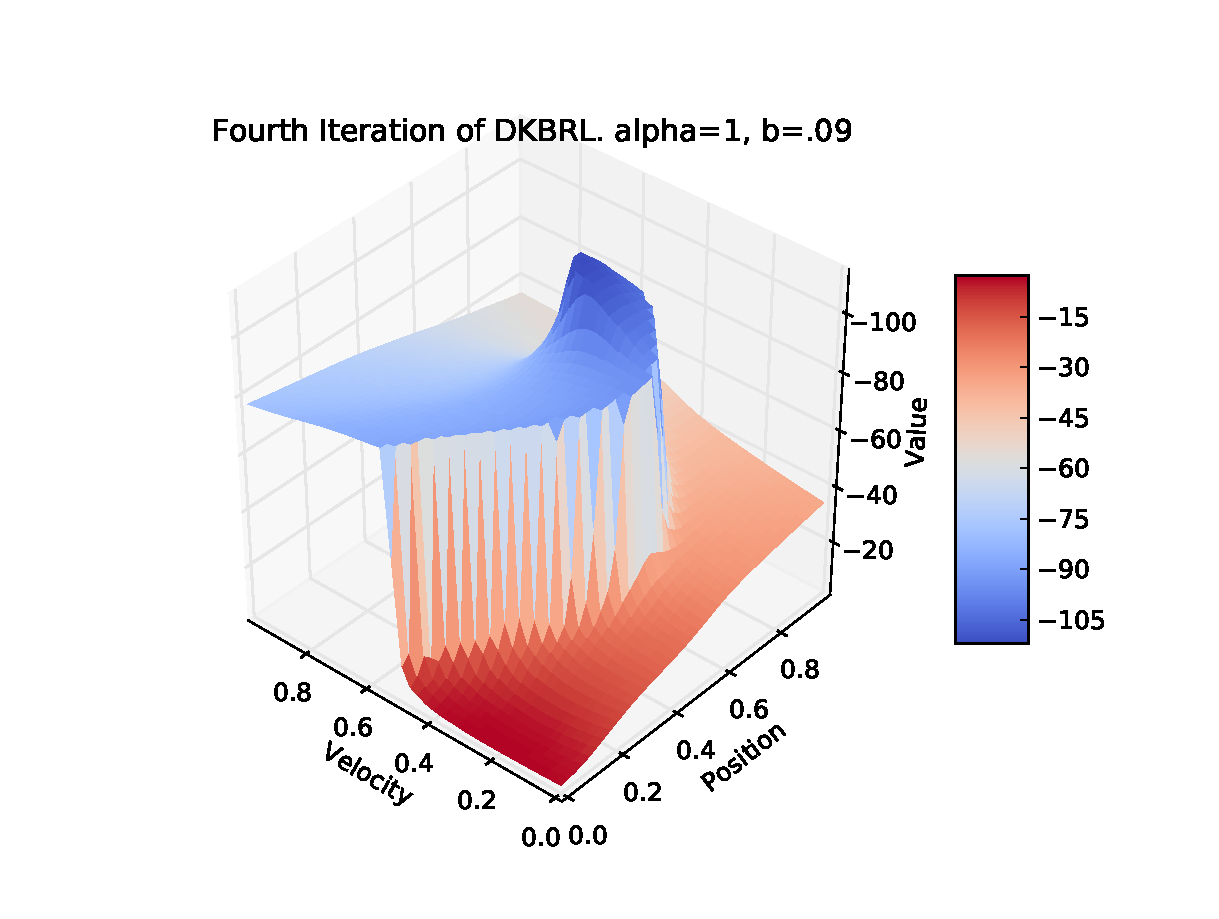
\includegraphics[width=\linewidth]{figs/chap5/mc09fourth.pdf}
  \endminipage
\caption[DKBRL approximation of Mountain-Car value function]
{On the left, Mountain-Car's value function as represented by KBRL.
On the right, Mountain-Car's value function after four iterations of DKBRL.
Both were made with the same set of transitions and a bandwidth of $.09$.
Note at how well DKBRL captures the discontinuity.
Also note the axes; the value DKBRL finds for the bottom of the hill
is closer to the true value of $-102$.}
\end{figure}

DKBRL is able to fit the value function well across a range of
bandwidths and sample sizes.
To see how this translates to solution quality I ran two types of experiments,
one holding the number of samples fixed and varying the bandwidth and
the other holding the bandwidth fixed and varying the number of samples.

\begin{figure}[!!!ht]
  \centering
    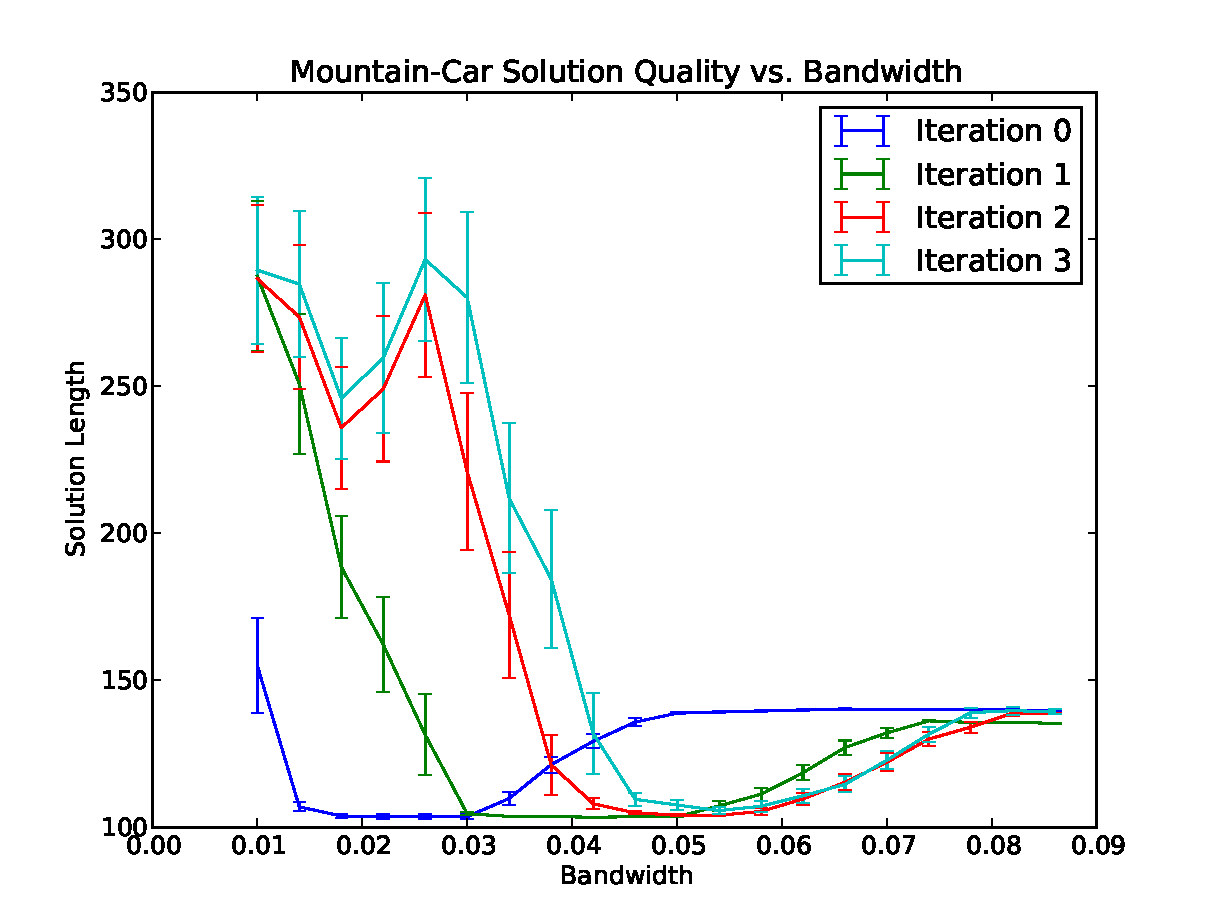
\includegraphics[width=90mm]{figs/chap5/mcband.pdf}
  \caption[Mountain-Car bandwidth sensitivity on each iteration of DKBRL]
{The average solution trajectory length on every iteration of
DKBRL. KBRL is equivalent to Iteration 0. The final solution returned by
DKBRL is the lower envelope of all the curves.}
\end{figure}

Figure 5-3 shows the sensitivity of the solution quality to the bandwidth
holding the sample size fixed at 600 transitions per action.
The graph shows the solution quality averaged over 40 trials.
Solution quality is measured as the length of the trajectory from start to
goal.
The error bars correspond to  one standard error.

Let us examine the features of this graph.
First note that KBRL (which corresponds to iteration 0)
is able to find the optimal solution when the bandwidth is in the
$.015$--$.03$ range. 
For these bandwidths, transforming makes the solution worse.
For larger bandwidths, FIIRA makes the solution better.
Note that there is a large difference in the curves for iteration 0 and
iteration 1.
This suggests that the setting $\alpha = 1$ is too high for this domain.

DKBRL retains the best policy it finds over all its iterations.
Thus, the final solution returned by DKBRL corresponds to the lower envelope of all
the curves in Figure 5-3.
Figure 5-4 plots this agianst the KBRL solution (which is equivalent to
Iteration 0) to see the extent of the improvement.
Note how DKBRL almost triples the range of bandwidths for which it is possible
to find the optimal trajectory.
Also note that DKBRL finds the optimal trajectory with lower
variance.

\begin{figure}[!!!ht]
  \centering
  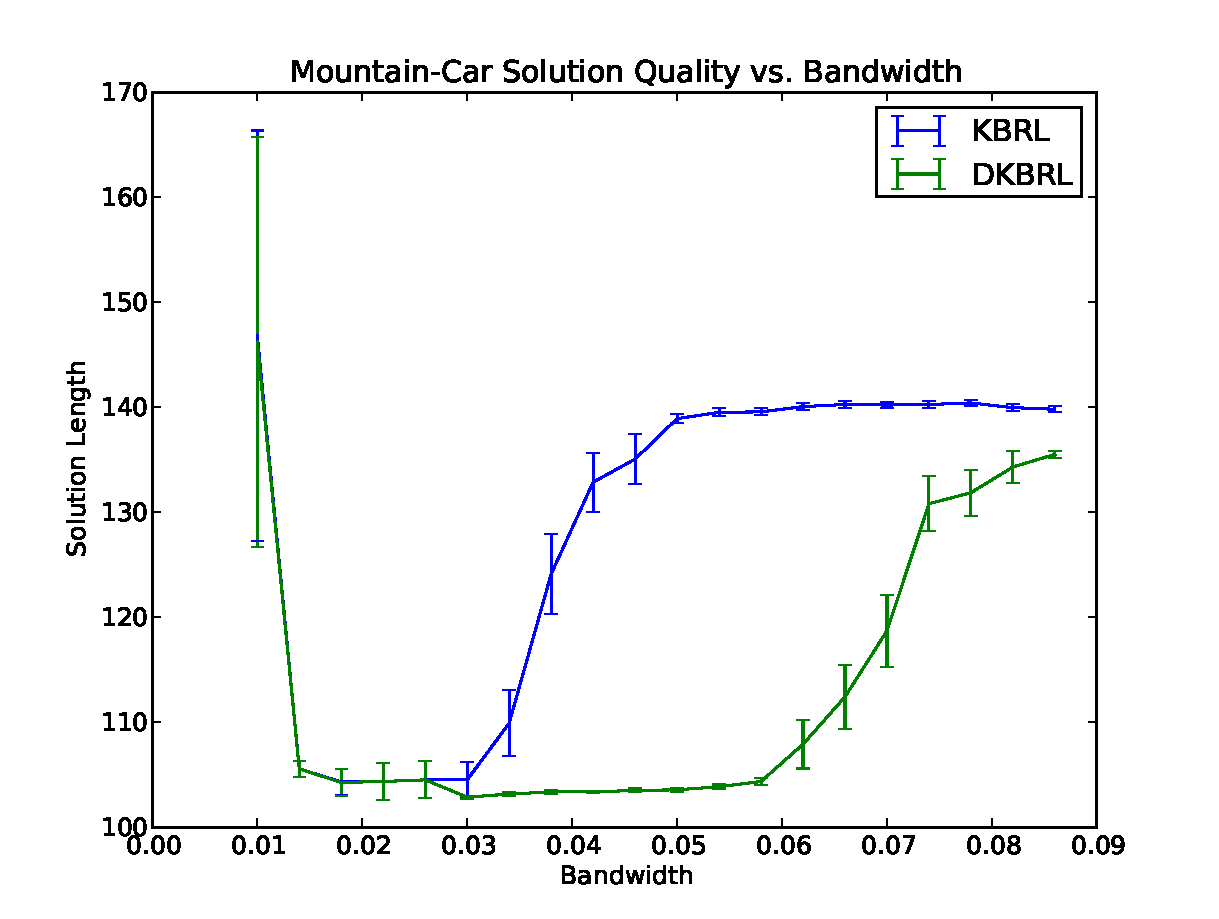
\includegraphics[width=90mm]{figs/chap5/mcband2.pdf}
  \caption[Bandwidth sensitivities of KBRL and DKBRL on Mountain-Car]
{The bandwidth sensitivities of KBRL and DKBRL on Mountain-Car.}
\end{figure}

The next three figures show the effect of sample size on solution quality
averaged over 20 trials for three different values of the bandwidth.
For small bandwidths, DKBRL is not able to improve upon KBRL.
For intermediate bandwidths, DKBRL greatly improves upon KBRL, which does not
manage to reach the optimal solution for any sample size.
On the other hand, given enough samples, DKBRL allows the agent to
consistently find the optimal solution.
Note that the DKBRL curve for $b=.05$ is slightly better than the
one for $b=.03$.
For large bandwidths, DKBRL improves on KBRL but does not find the optimal
solution consistently.
I conjecture that this is because we are approaching minimum
bandwidth needed to adequately model the dynamics of the system.

\begin{figure}[!!!ht]
  \centering
    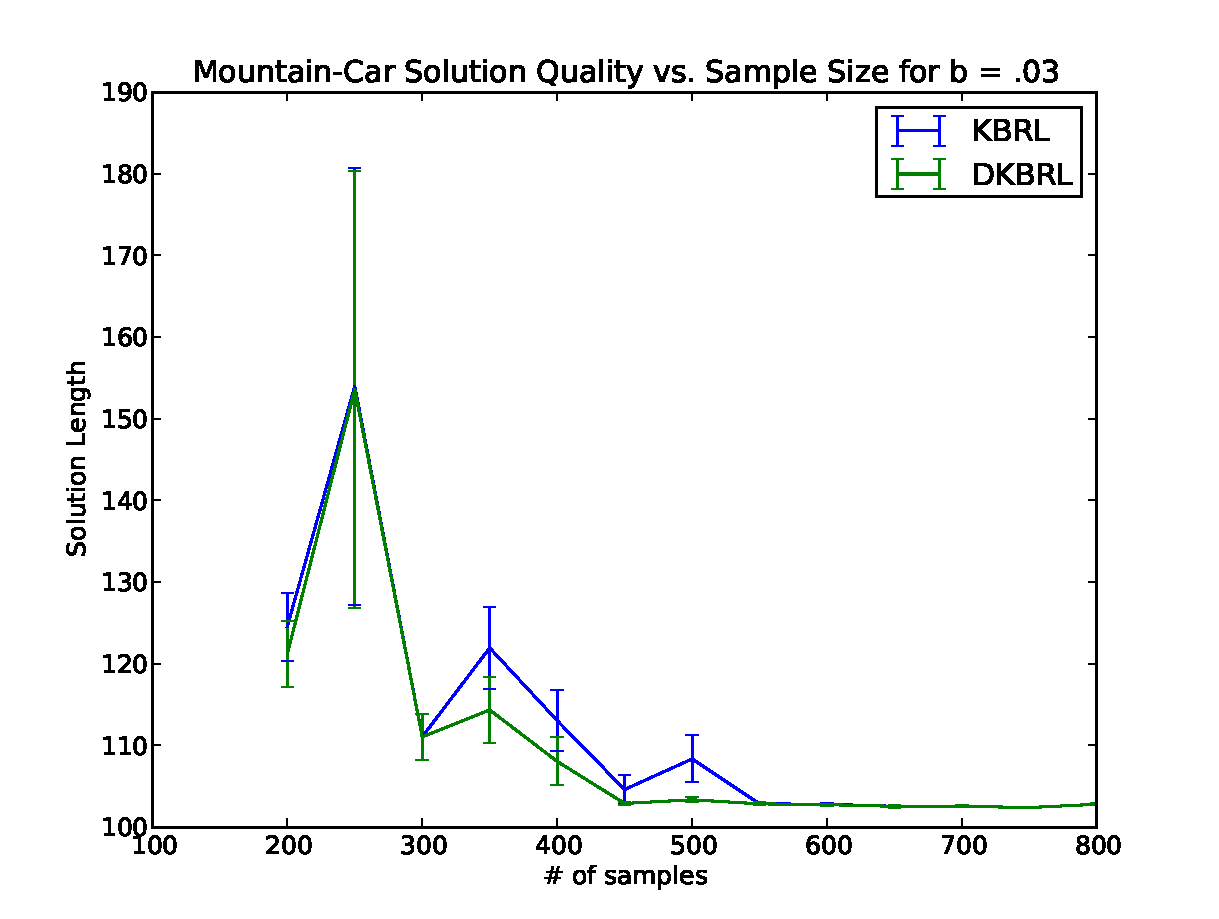
\includegraphics[width=75mm]{figs/chap5/mc03.pdf}
  \caption[KBRL vs. DKBRL with small bandwidth on Mountain-Car]
{DKBRL does not improve upon KBRL when the bandwidth is small.}
\end{figure}
\begin{figure}[!!!ht]
  \centering
    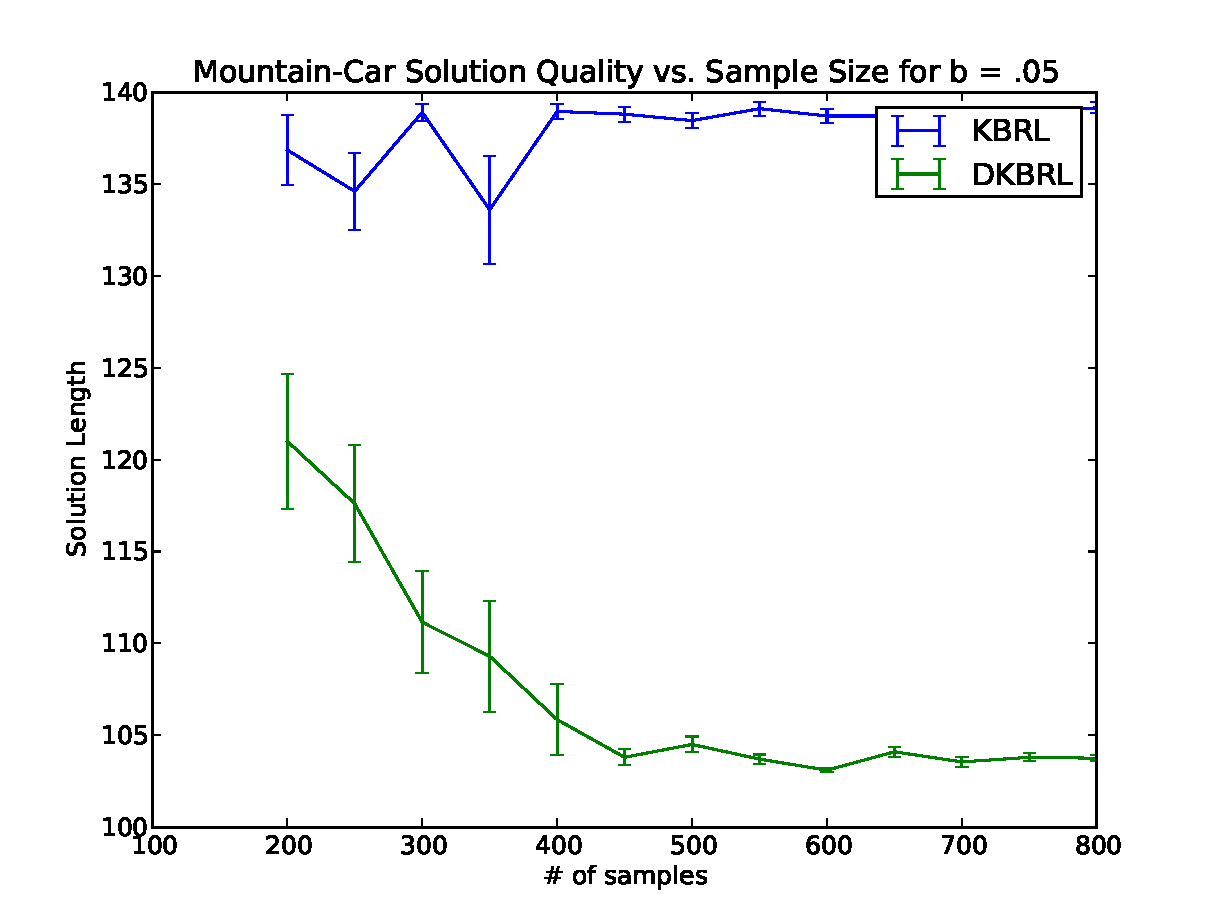
\includegraphics[width=75mm]{figs/chap5/mc05.pdf}
  \caption[KBRL vs. DKBRL with itermediate bandwidth on Mountain-Car]
  {DKBRL significantly improves upon KBRL when the bandwidth is
intermediate.}
\end{figure}
\begin{figure}[!!!ht]
  \centering
    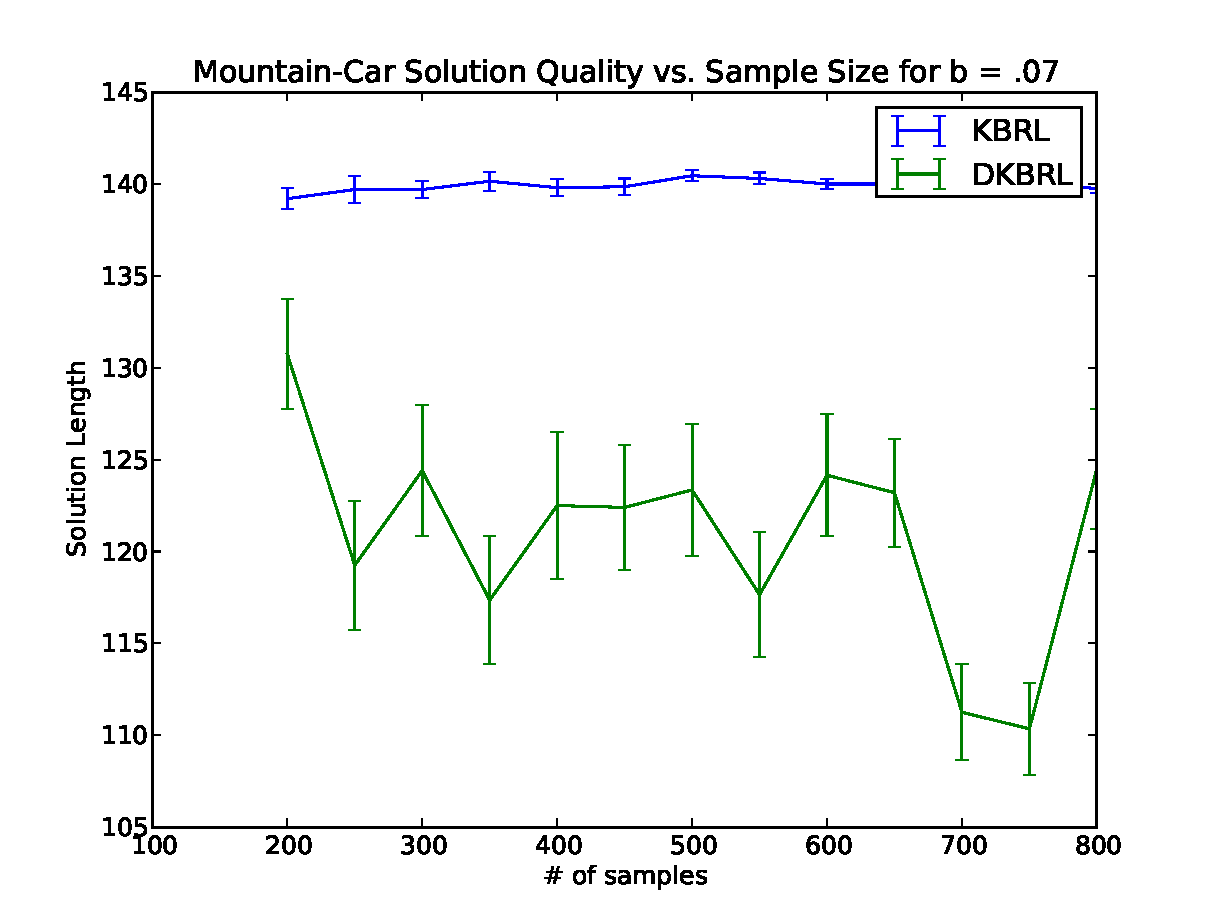
\includegraphics[width=75mm]{figs/chap5/mc07.pdf}
  \caption[KBRL vs. DKBRL with large bandwidth on Mountain-Car]
{DKBRL improves upon KBRL when the bandwidth is large, but not as
much as it does when the bandwidth is intermediate.}
\end{figure}

These experiments show that DKBRL is capable of improving upon the solution
generated by KBRL.
This improvement in the solution quality is not as large as the improvement in the
value function approximation.
This is because representing the value function well is not necessary for
solving Mountain-Car (or any MDP in general).
All that matters is that the best action gets assigned the highest Q-Value.
This means DKBRL might not produce a better policy even if it improves on
the value function approximation.
In fact, it can produce a worse policy if it changes the ranking of the actions
in the wrong direction.

\section{Acrobot}
Acrobot is a four dimensional MDP by Sutton and Barton \cite{rlai}.
It models a two-link, underactuated robot that is anchored at one end,
similar to a gymnast on a high bar.
The agent's objective is to get its leg above some height.

The four dimensions correspond to the angles and angular velocities of the two
links.
There are three discrete actions (LEFT, RIGHT, and IDLE) corresponding to
how the agent can actuate the joint between the two links.
The code I used was adapted from \cite{rlglue}
The best solution trajectory I observed during my experiments 112 steps long.

\begin{figure}[!!!ht]
  \centering
    \includegraphics[width=30mm]{figs/abexpl.png}
  \caption[Acrobot domain]{Picture of the Acrobot domain
(taken from rl-community.org, available under GNU FDL)}
\end{figure}

To evaluate DKBRL's performance on Acrobot, I repeated the experiments I did
on Mountain-Car.
In the first set of experiments, I set the number of samples fixed at 3000
transitions per action and varied the bandwidth.
The results (Figure 5-9) showed that the optimal number of iterations was
different at different bandwidths.
Iteration 0 (KBRL) does not appear to be optimal anywhere, though the error bars
are too large to be sure.

\begin{figure}[!!!ht]
  \centering
    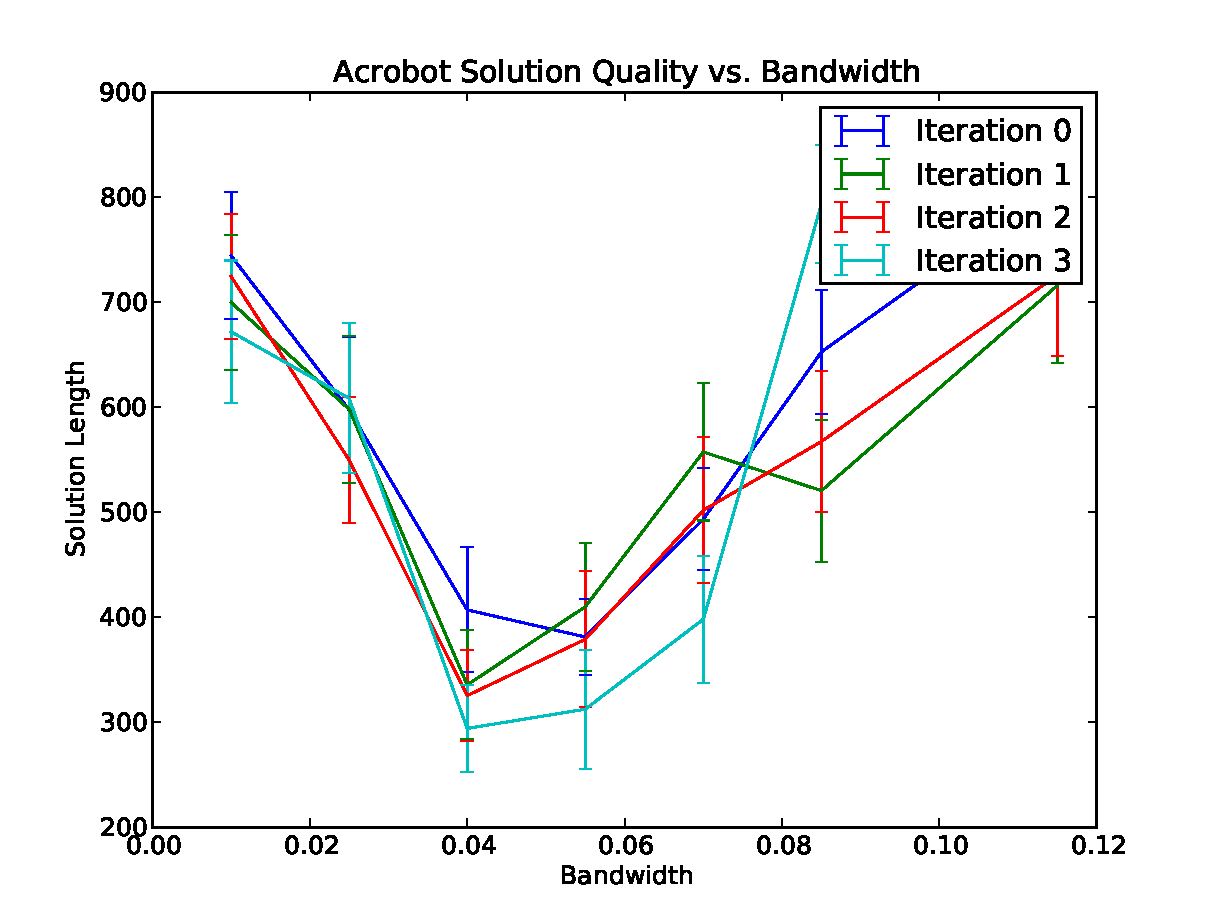
\includegraphics[width=90mm]{figs/chap5/acroband.pdf}
  \caption[Acrobot bandwidth sensitivity on each iteration of DKBRL]
{Solution quality vs. bandwidth over four iterations of DKBRL,
  averaged over 20 trails.}
\end{figure}

To see how DKBRL compares to KBRL, we can again plot the lower envelope of
all the iterations against Iteration 0. This is shown in Figure 5-10.
Note how DKBRL is able to find better solutions across all bandwidths.
Be aware that an average solution length of 900 does not mean the solver was
finding paths that were 900 steps long.
It means that in most episodes the agent could not reach the goal
(these are treated as 1000) and in three or four episodes the agent reached
the goal quickly.
This is why the standard errors are so high.

\begin{figure}[!!!ht]
  \centering
    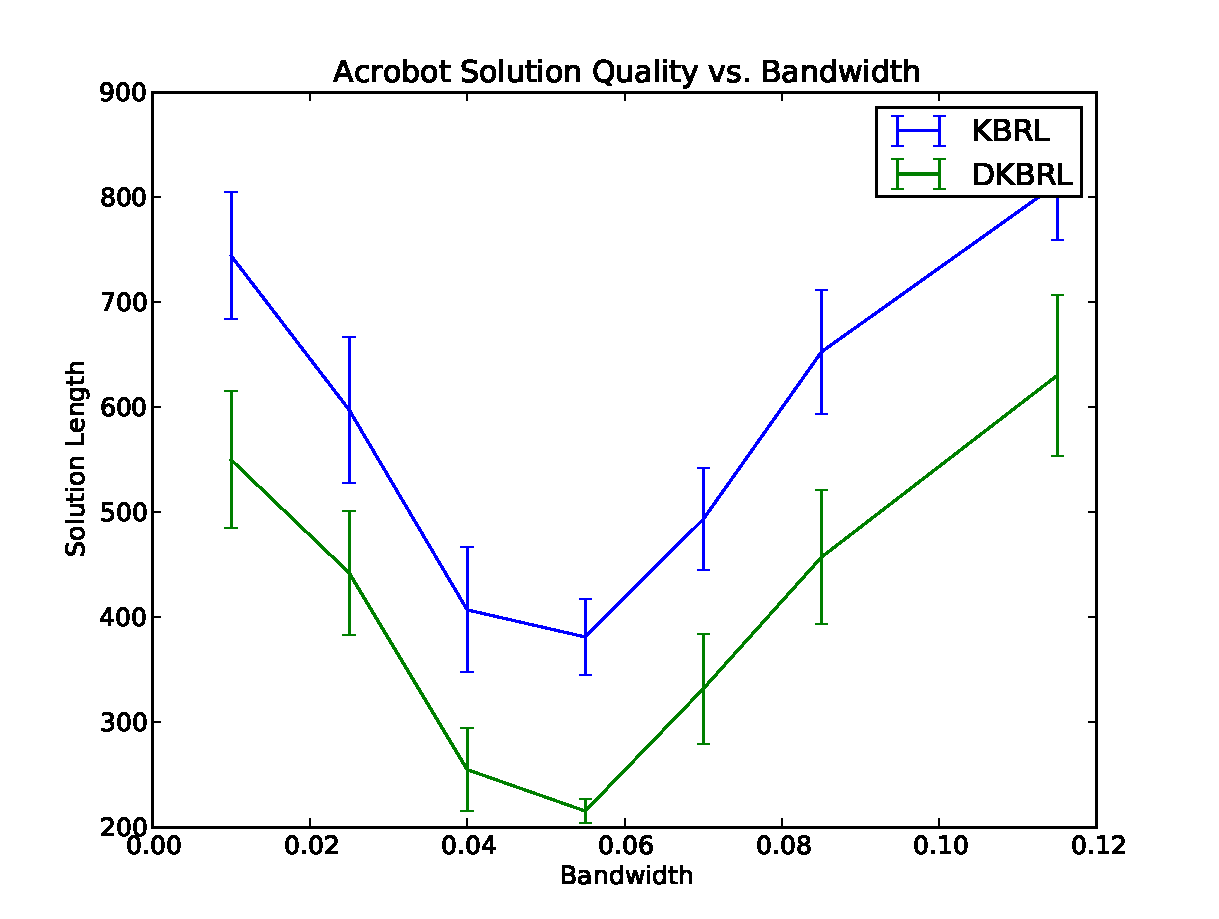
\includegraphics[width=90mm]{figs/chap5/acroband2.pdf}
  \caption[Bandwidth sensitivities of KBRL and DKBRL on Acrobot]
{The bandwidth sensitivities of KBRL and DKBRL on Acrobot.}
\end{figure}

The next set of experiments held the bandwidth fixed and varied the number of
samples.
The results of these are shown in Figure 5-11.
Note how DKBRL produces substantially better solutions for all sample size and bandwidth
combinations.
Still, DKBRL was not able to consistently find the optimal solution.

\begin{figure}[!htb]
  \minipage{0.33\textwidth}
    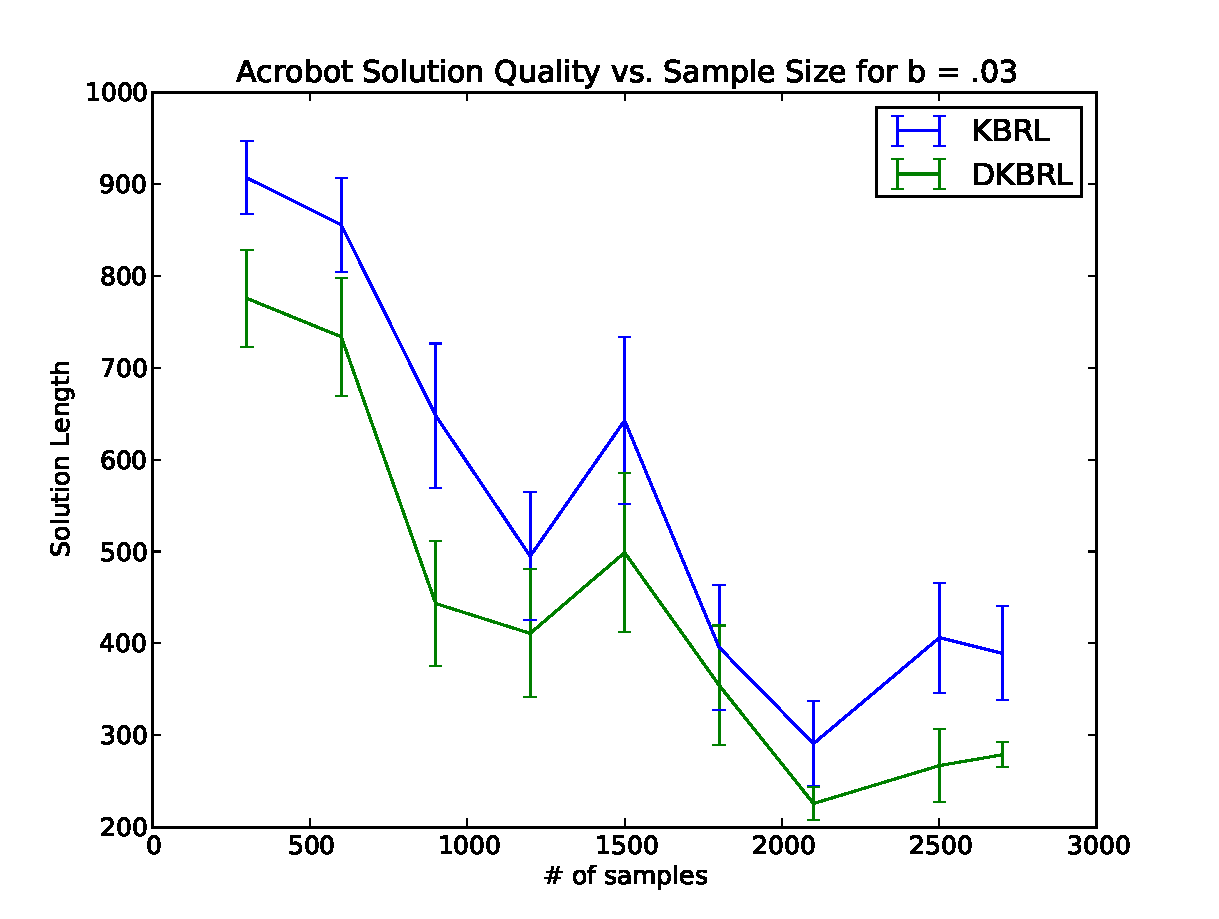
\includegraphics[width=\linewidth]{figs/chap5/acr03.pdf}
  \endminipage\hfill
  \minipage{0.33\textwidth}
    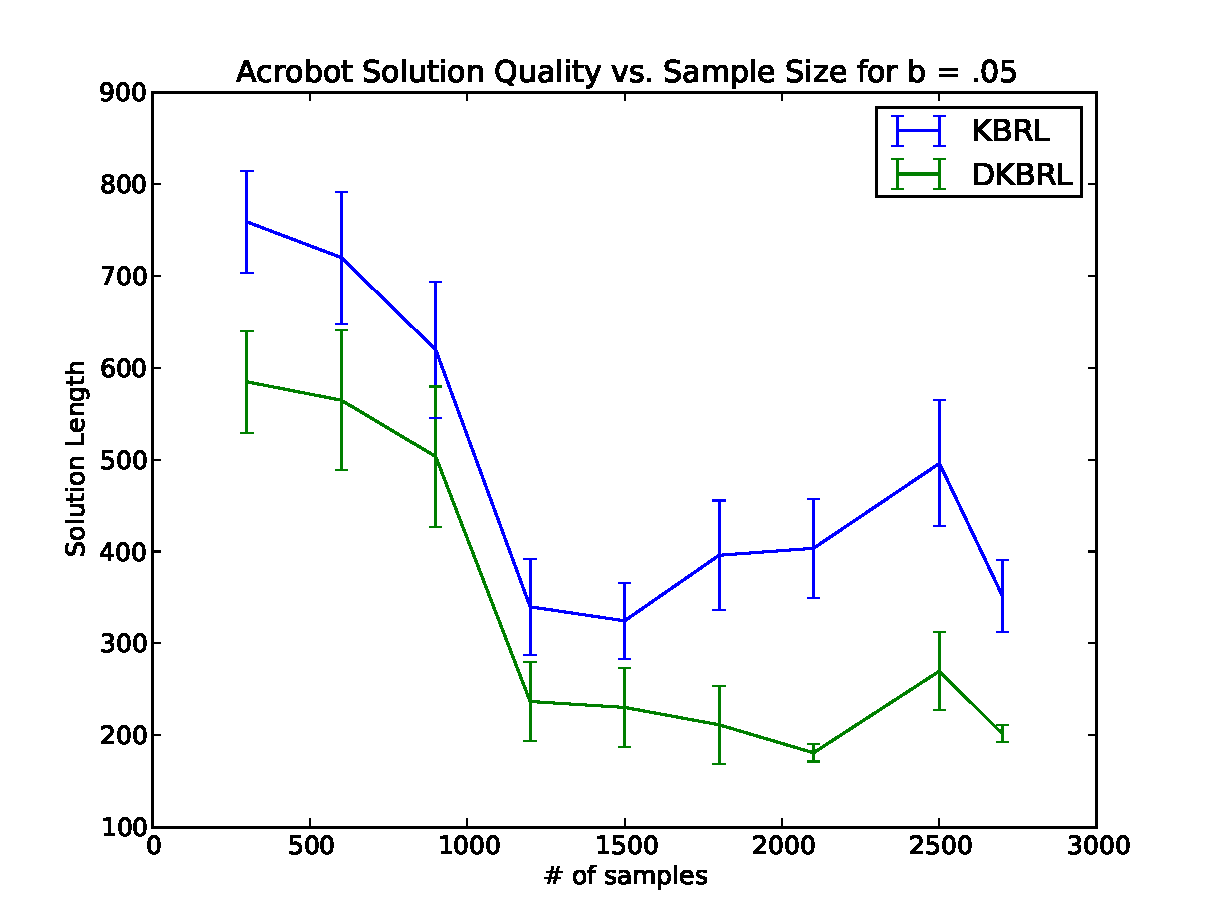
\includegraphics[width=\linewidth]{figs/chap5/acr05.pdf}
  \endminipage\hfill
  \minipage{0.33\textwidth}
    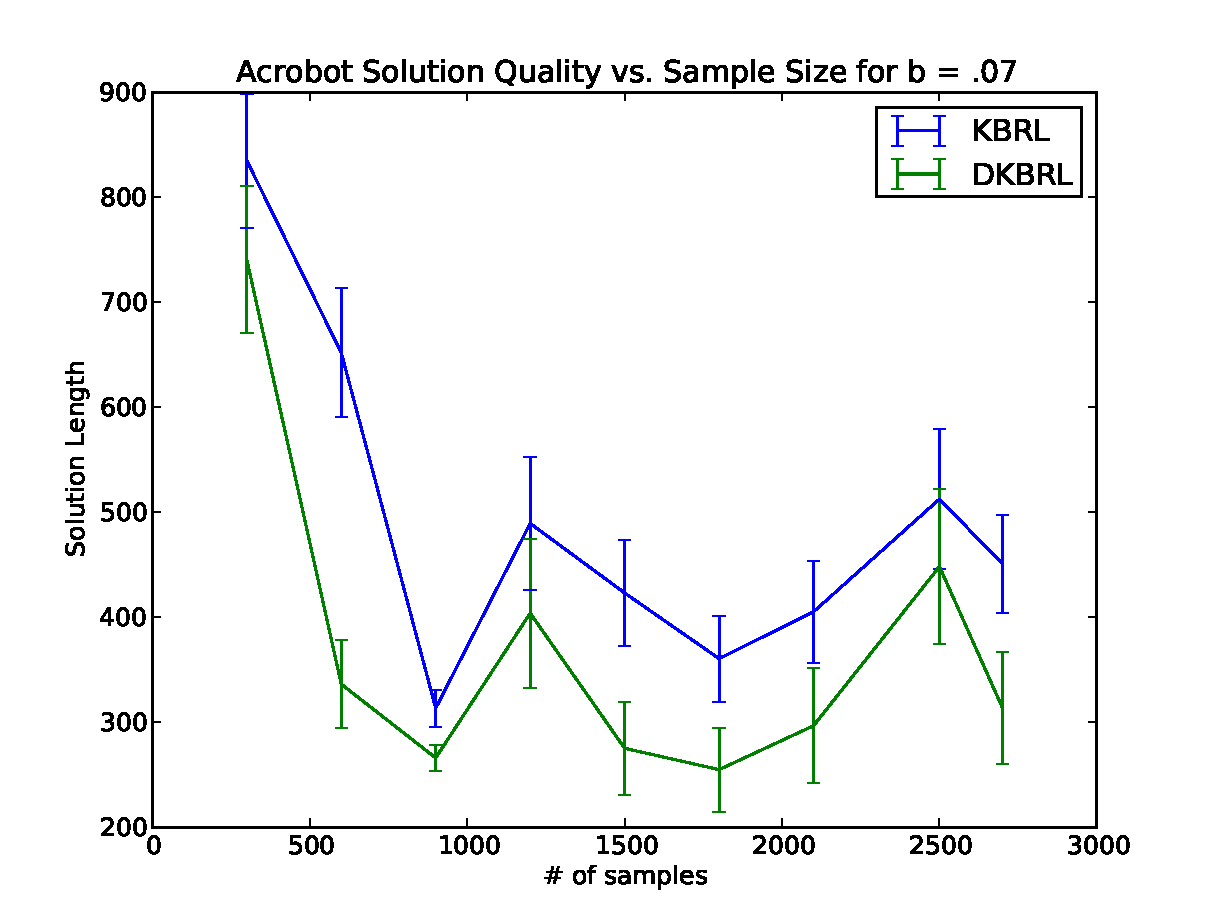
\includegraphics[width=\linewidth]{figs/chap5/acr07.pdf}
  \endminipage
\caption[KBRL vs. DKBRL on Acrobot]
{The solution qualities of KBRL and DKBRL for different bandwidths
and number of samples averaged over 20 trials.}
\end{figure}

These experiments showed that DKBRL is able to produce substantial improvements
in solution quality when performed on Acrobot.
This suggests that representing the value function correctly is more
important in Acrobot than in Mountain-Car.

\section{PinBall}
PinBall is an even more challenging 4D MDP described in \cite{gdk}.
In PinBall, the agent models a ball trying to navigate through a maze towards
a goal.
The agent has five actions, UP, DOWN, LEFT, RIGHT, and COAST.
The agent incurs a penalty when taking one of the first four actions.
To navigate efficently, the agent must bounce off the obstacles to change
direction without accelerating.

\begin{figure}[!!!ht]
  \centering
    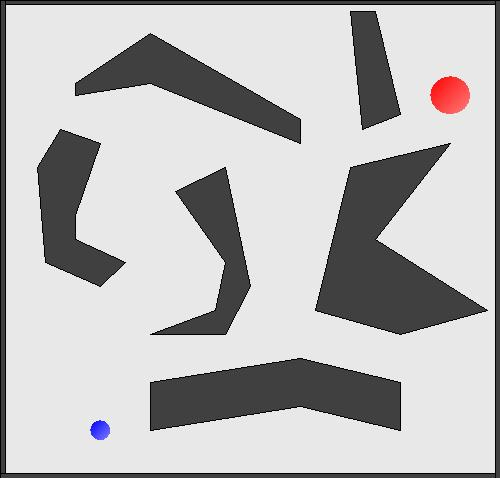
\includegraphics[width=60mm]{figs/chap5/pbeasy.jpg}
  \caption[PinBall domain map]{Map of the PinBall domain.
The start point is marked in blue and the end point in red.
(Picture taken from http://www-all.cs.umass.edu/~gdk/pinball/ with permission)}
\end{figure}

In PinBall, a random walk does not provide good coverage of the state space.
This is because the ball never builds up momentum and high velocity states do
not get reached.
To get around this, I sampled ball positions for reachability and velocities
at random.

PinBall is a challenging domain because the volume of the reachable state space
is much higher than that of Acrobot.
It is also filled with narrow corridors that are difficult to pass through
without a good policy.

PinBall is an especially interesting domain because, it allows for more
intricate transforms.
In PinBall, variation in velocity does not affect the value of a state nearly
as much as variation in position.
Two points with the same velocity but large difference in position will have
a greater difference in value that points with the same position and large
difference in velocity.
This means a good transform will squash the space along the velocity
dimensions.
This reduces the volume of the state space making the problem easier to solve.

Because PinBall is such a difficult domain, solving it non-parametrically is
extremely computation intensive.
As a result, I could not perform the same type of tests I did for Mountain-Car
and Acrobot. Instead I picked some settings of parameters and ran a few trials
of the algorithm.

For the first batch of tests I chose to use DKBSF.
Since Barreto et. al. \cite{kbsf} give no guidance on the optimal ratio of sample
transitions to representative points for a given amount of compute time,
I had to pick these arbitrarily.
I collected 30000 sample transitions per action and 5000 representative points 
and chose a bandwidth of .03 \footnote{The sample size was set by the amount of
memory available on the machine used for the experiments and the bandwidth was 
the smallest number that didn't result in arithmetic underflows when
evaluating the kernel}.
Each trial took roughly a day to perform.

\begin{table}[H]
\begin{center}
    \begin{tabular}{| l | l | l | l |}
    \hline
Trial & Alpha & Iter. 0 & Iter. 1 \\ \hline
0 & .16 & -- & 360\\
1 & .16 & -- & 230\\
2 & .25 & -- & 235\\
3 & .25 & -- & 245\\
4 & .16 & 157 & ERROR\\
5 & .16 & -- & --\\
6 & .16 & -- & --\\
7 & .16 & 252 & 176\\
8 & .16 & -- & 169\\
9 & .16 & -- & --\\
10 & .16 & -- & --\\
    \hline
    \end{tabular}
\end{center}
    \caption[DKBSF Pinball results]
{The number of steps to reach the goal in 11 trials of DKBSF on PinBall.
A ``--'' means the agent did not reach the goal.}
\end{table}

Table 5.1 shows the result of this experiment.
A ``--'' means the ball did not make it to the goal.
An ``ERROR'' means the program crashed mid computation\footnote{There was
supposed to be a column for Iteration 2 but it was full of ``ERROR''s and
is omitted.}.
As before, Iteration 0 is equivalent to KBSF and the subsequent iterations
show the improvement resulting from DKBSF.
From this table, it appears DKBSF is offering some advantage, though it is
not possible to say how much.
KBSF was only able to reach the goal in 2 out of 11 trials while DKBSF did so
in 6 out of 10.

\begin{figure}[!!!ht]
  \centering
    \includegraphics[width=90mm]{figs/apdx/f1.png}
  \caption[DKBSF on PinBall sample trajectory]{The trajectories generated
on trial 1. Iteration 0 (KBSF) is on the left and iteration 1 (DKBSF) is on
the right. The path is colored by time; a full cycle through the hues
corresponds to 100 steps.
Note how KBSF misses the narrow corridor then attempts to go through the wall
while DKBSF makes it through. The remaining trajectories are in the appendix. }
\end{figure}

For the next batch of experiments, I tried DKBRL with a sample size of
10000 transitions per action and a bandwidth of $.15$.
The results of that experiment are shown in Table 5.2.

\begin{table}[H]
\begin{center}
    \begin{tabular}{| l | l | l | l | l |}
    \hline
Exp\# & Alpha & Iter. 0 & Iter. 1 & Iter 2. \\ \hline
0 & 1 & -- & 243 & --\\
1 & 1 & -- & -- & --\\
2 & 1 & -- & -- & --\\
3 & 1 & -- & 356 & --\\
4 & 1 & -- & -- & --\\
5 & 1 & -- & 294 & --\\
6 & 1 & -- & 377 & --\\
7 & 1 & -- & 258 & --\\
8 & 1 & -- & 429 & --\\
9 & 1 & -- & 332 & --\\
10& 1 & 255 & 382 & --\\
    \hline
    \end{tabular}
\end{center}
    \caption[DKBRL PinBall results]{The results of running DKBRL on PinBall.}
\end{table}

The results of this experiment are similar to those for KBSF.
Using KBRL alone, the ball was only able to get the goal once out of eleven
trials; however, after a single iteration of DKBRL the ball made it on
eight trials.
Performing an additional iteration made the performance worse.\\

\begin{figure}[!!!ht]
  \centering
    \includegraphics[width=110mm]{figs/apdx/r0.png}
  \caption[DKBRL on PinBall sample trajectory]{The trajectories generated
on trial 0. KBSF attempts to go straight up,
iteration 1 of DKBSF goes around around all the obstacles,
iteration 2 gets stuck in a corner. Most of the trials looked very similar to this.}
\end{figure}

\begin{figure}[!!!ht]
  \centering
    \includegraphics[width=110mm]{figs/apdx/r10.png}
  \caption[DKBRL on PinBall sample trajectory 2]{The trajectories generated
on trial 10, the only trajectory where KBRL reached the goal.}
\end{figure}

Together, the experiments in this chapter show that FIIRA is capable of
offering tangible performance improvements when applied to KBRL.
\chapter{Conclusions and Future Work}
The way a problem is represented can have a substantial impact on how difficult
it is to solve.
The right representation can make short work of a seemingly complicated
problem.
A good representation is one that is highly correlated with value.
Existing algorithms for representation discovery do not explicitly take value
into consideration and thus cannot discover such a representation in most
situations.
This thesis introduced an iterative representation discovery algorithm that
interleaves steps of value approximation and representation updates.
This algorithm was effective across a range of problems, including three
benchmark reinforcement learning problems.
The work in this thesis opens several exciting avenues for future research.

The first and most natural next step from this thesis is a thorough exploration
of the properties of the FIIRA framework.
It would be interesting to see how different combinations of regressors and
transformers work together.
It would be particularly interesting to see the results of performing FIIRA in
a parametric reinforcement learning setting.
Such an exploration could result in formal proofs about FIIRA's properties.

Another possible next step would be an in-depth study of the applicability of
sustained actions to KBRL.
Sustained actions were instrumental in the experiments detailed in Chapter 5,
especially in the PinBall domain.
Without sustained actions, the number of sample transitions needed to cover
the space would have exceeded the available computational resources.
I firmly believe that there is some fundamental principle behind sustained
actions that makes them worth studying.

Yet another possible direction would be to seek out new applications for FIIRA.
This thesis discusses only reinforcement learning, but FIIRA could be applied
in other function approximation tasks.
The particular FIIRA algorithm described in this thesis could also be used as
a clustering algorithm.
It collapses the domain into a finite set of atoms and has been demonstrated
effective at identifying discontinuities.
This suggests potential as an algorithm for clustering by value.

\appendix
\chapter{Proofs}
This section contains two proofs that were omitted from section 4.3.

\begin{claim}Any dataset $D = \{(x_1, y_1), (x_2, y_2)\}$ with $x_1 \neq x_2$
and $y_1 \neq y_2$ is a stable fixed point of FDK for any choice of kernel if
the
domain is taken to be the set $\{x_1, x_2\}$ (i.e. no
interpolation between the two points).\end{claim}

\begin{proof}The diameter of the domain is $\|x_1 - x_2\|$. Since
\textit{DAWIT} is diameter preserving, the two points in the domain do not
move relative to each other after the transformation.
It follows that $\|\Phi(x_1) - \Phi(x_2)\| = \|x_1 - x_2\|$ and thus
$\tilde f_1(x) = \tilde f_2(\Phi_1(x))$ for both $x_1$ and
$x_2$, making $D$ a fixed point of FDK.
Note that $D$ is not an attractive fixed point: if the
$x_i$ are perturbed, the result is a new fixed point.\end{proof}

\begin{claim}When done using a kernel, $k$, with compact support having
bandwidth,
$b < \frac{\mathrm{diam}(X)}{c}$ for some integer, $c$, FDK has a stable, attractive fixed point with
$c + 1$ atoms.\end{claim}

\begin{proof}(by construction)
Consider the dataset $D = \{(x_i,y_i)\ |\ i = 0\ldots c\}$ with $x_i = y_i = ic$.
We show that performing a round of FDK does not move the $x_i$ relative to
eachother, making $D$ a fixed point.

Solving for $\tilde f_0$ gives $$\tilde f_0(x) = \sum_i k(x,x_i)y_i = y_i.$$
Note that the value predicted for each $x_i$ is independent of $x_j\ \forall
j\neq i$. This is because a kernel centered on one point does not reach any
of the others.
Further note that $\tilde f_0$ is a line, making $D$ a fixed point 

To show that $D$ is an attractive fixed point, purturb every $x_i$ in the
domain by some $\epsilon_i$, setting $x_i' = x_i + \epsilon_i$.
If each $|\epsilon_i| < \frac{\mathrm{diam}(X)}{c} - b$,
it will still be the case that $\tilde f(x_i') = y_i$.
To straigten out $\tilde f$, the WIT will push each $x_i'$ closer to $x_i$.
This makes $D$ an attractive fixed point.
\end{proof}

The proof above shows that as the bandwidth shrinks, the number of atoms
increases.
This implies that the piecewise flat approximations generated with a
smaller bandwidth will have more pieces.
The proof can be extended to deal with kernels without compact support.

\clearpage
\newpage

\chapter{PinBall Trajectories}
This section shows the trajectories generated by KBSF (left) and DKBSF (right).
Each picture corresponds to a row in Table 5.1.
The trajectories generated by KBRL and DKBRL are not shown because they
were so similar to the ones in Figure 5-14.

\begin{figure}[!!!ht]
  \centering
    \includegraphics[width=110mm]{figs/apdx/f0.png}
\end{figure}

\begin{figure}[!!!ht]
  \centering
    \includegraphics[width=110mm]{figs/apdx/f1.png}
\end{figure}

\begin{figure}[!!!ht]
  \centering
    \includegraphics[width=110mm]{figs/apdx/f2.png}
\end{figure}

\begin{figure}[!!!ht]
  \centering
    \includegraphics[width=110mm]{figs/apdx/f3.png}
\end{figure}

\begin{figure}[!!!ht]
  \centering
    \includegraphics[width=110mm]{figs/apdx/f4.png}
\end{figure}

\begin{figure}[!!!ht]
  \centering
    \includegraphics[width=110mm]{figs/apdx/f5.png}
\end{figure}

\begin{figure}[!!!ht]
  \centering
    \includegraphics[width=110mm]{figs/apdx/f6.png}
\end{figure}

\begin{figure}[!!!ht]
  \centering
    \includegraphics[width=110mm]{figs/apdx/f7.png}
\end{figure}

\begin{figure}[!!!ht]
  \centering
    \includegraphics[width=110mm]{figs/apdx/f8.png}
\end{figure}

\begin{figure}[!!!ht]
  \centering
    \includegraphics[width=110mm]{figs/apdx/f9.png}
\end{figure}

\begin{figure}[!!!ht]
  \centering
    \includegraphics[width=110mm]{figs/apdx/f10.png}
\end{figure}

%% This defines the bibliography file (main.bib) and the bibliography style.
%% If you want to create a bibliography file by hand, change the contents of
%% this file to a `thebibliography' environment.  For more information 
%% see section 4.3 of the LaTeX manual.
\begin{singlespace}
\bibliography{main}
\bibliographystyle{plain}
\end{singlespace}

\end{document}

